\begin{minipage}[b]{0.15\linewidth}
\begin{figure}[H]                                                          
  \centering                                                             
  \begin{adjustbox}{width=1.5cm,center}                                   
  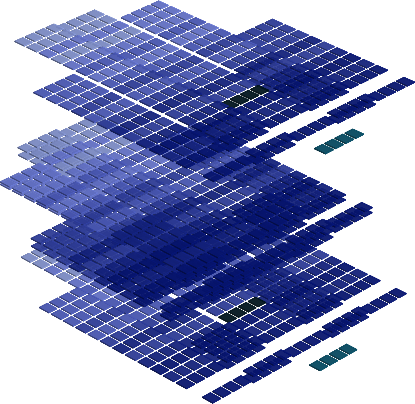
\includegraphics[width=1.5cm]{src/colorspace_colourflow/flows/colourflow_130-45.png}%           
  \end{adjustbox}                                                        
\caption*{

\begin{tikzpicture}                             
\definecolor{tempcolor}{HTML}{000000}           
\fill[tempcolor] (1 mm,0) rectangle ++(1mm,1mm);
\definecolor{tempcolor}{HTML}{081b90}           
\fill[tempcolor] (2 mm,0) rectangle ++(1mm,1mm);
\definecolor{tempcolor}{HTML}{192ca1}           
\fill[tempcolor] (3 mm,0) rectangle ++(1mm,1mm);
\definecolor{tempcolor}{HTML}{3b4ec3}           
\fill[tempcolor] (4 mm,0) rectangle ++(1mm,1mm);
\definecolor{tempcolor}{HTML}{5d70e5}           
\fill[tempcolor] (5 mm,0) rectangle ++(1mm,1mm);
\definecolor{tempcolor}{HTML}{7f92ff}           
\fill[tempcolor] (6 mm,0) rectangle ++(1mm,1mm);
\definecolor{tempcolor}{HTML}{a1b4ff}           
\fill[tempcolor] (7 mm,0) rectangle ++(1mm,1mm);
\definecolor{tempcolor}{HTML}{c3d6ff}           
\fill[tempcolor] (8 mm,0) rectangle ++(1mm,1mm);
\end{tikzpicture}                               
}
\end{figure}                                                               
\end{minipage}
\hspace{0.1cm}
\begin{minipage}[b]{0.15\linewidth}
\begin{figure}[H]                                                          
  \centering                                                             
  \begin{adjustbox}{width=1.5cm,center}                                   
  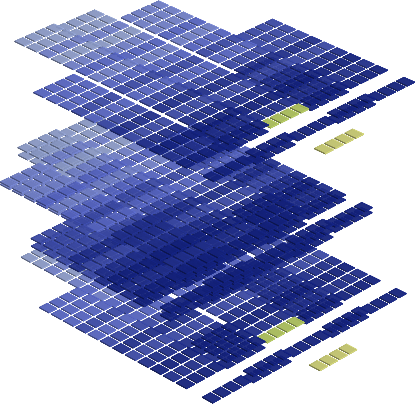
\includegraphics[width=1.5cm]{src/colorspace_colourflow/flows/colourflow_131-45.png}%           
  \end{adjustbox}                                                        
\caption*{

\begin{tikzpicture}                             
\definecolor{tempcolor}{HTML}{000000}           
\fill[tempcolor] (1 mm,0) rectangle ++(1mm,1mm);
\definecolor{tempcolor}{HTML}{192ca1}           
\fill[tempcolor] (2 mm,0) rectangle ++(1mm,1mm);
\definecolor{tempcolor}{HTML}{2a3db2}           
\fill[tempcolor] (3 mm,0) rectangle ++(1mm,1mm);
\definecolor{tempcolor}{HTML}{4c5fd4}           
\fill[tempcolor] (4 mm,0) rectangle ++(1mm,1mm);
\definecolor{tempcolor}{HTML}{6e81f6}           
\fill[tempcolor] (5 mm,0) rectangle ++(1mm,1mm);
\definecolor{tempcolor}{HTML}{90a3ff}           
\fill[tempcolor] (6 mm,0) rectangle ++(1mm,1mm);
\definecolor{tempcolor}{HTML}{b2c5ff}           
\fill[tempcolor] (7 mm,0) rectangle ++(1mm,1mm);
\definecolor{tempcolor}{HTML}{d4e7ff}           
\fill[tempcolor] (8 mm,0) rectangle ++(1mm,1mm);
\end{tikzpicture}                               
}
\end{figure}                                                               
\end{minipage}
\hspace{0.1cm}
\begin{minipage}[b]{0.15\linewidth}
\begin{figure}[H]                                                          
  \centering                                                             
  \begin{adjustbox}{width=1.5cm,center}                                   
  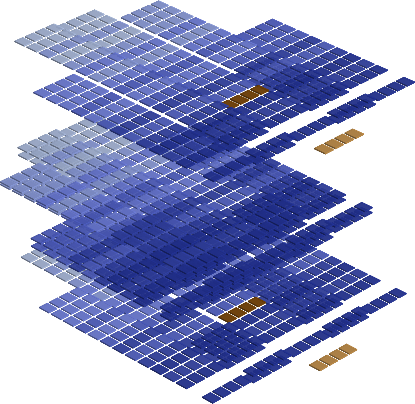
\includegraphics[width=1.5cm]{src/colorspace_colourflow/flows/colourflow_132-45.png}%           
  \end{adjustbox}                                                        
\caption*{

\begin{tikzpicture}                             
\definecolor{tempcolor}{HTML}{000000}           
\fill[tempcolor] (1 mm,0) rectangle ++(1mm,1mm);
\definecolor{tempcolor}{HTML}{2a3db2}           
\fill[tempcolor] (2 mm,0) rectangle ++(1mm,1mm);
\definecolor{tempcolor}{HTML}{3b4ec3}           
\fill[tempcolor] (3 mm,0) rectangle ++(1mm,1mm);
\definecolor{tempcolor}{HTML}{5d70e5}           
\fill[tempcolor] (4 mm,0) rectangle ++(1mm,1mm);
\definecolor{tempcolor}{HTML}{7f92ff}           
\fill[tempcolor] (5 mm,0) rectangle ++(1mm,1mm);
\definecolor{tempcolor}{HTML}{a1b4ff}           
\fill[tempcolor] (6 mm,0) rectangle ++(1mm,1mm);
\definecolor{tempcolor}{HTML}{c3d6ff}           
\fill[tempcolor] (7 mm,0) rectangle ++(1mm,1mm);
\definecolor{tempcolor}{HTML}{e5f8ff}           
\fill[tempcolor] (8 mm,0) rectangle ++(1mm,1mm);
\end{tikzpicture}                               
}
\end{figure}                                                               
\end{minipage}
\hspace{0.1cm}
\begin{minipage}[b]{0.15\linewidth}
\begin{figure}[H]                                                          
  \centering                                                             
  \begin{adjustbox}{width=1.5cm,center}                                   
  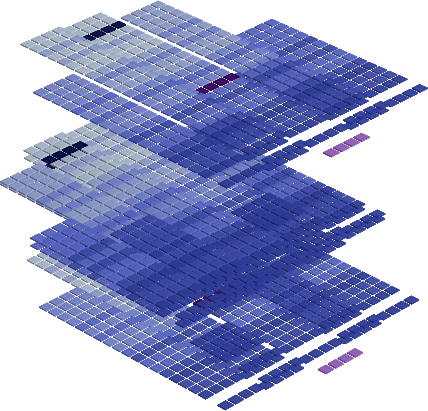
\includegraphics[width=1.5cm]{src/colorspace_colourflow/flows/colourflow_133-45.png}%           
  \end{adjustbox}                                                        
\caption*{

\begin{tikzpicture}                             
\definecolor{tempcolor}{HTML}{000000}           
\fill[tempcolor] (1 mm,0) rectangle ++(1mm,1mm);
\definecolor{tempcolor}{HTML}{3b4ec3}           
\fill[tempcolor] (2 mm,0) rectangle ++(1mm,1mm);
\definecolor{tempcolor}{HTML}{4c5fd4}           
\fill[tempcolor] (3 mm,0) rectangle ++(1mm,1mm);
\definecolor{tempcolor}{HTML}{6e81f6}           
\fill[tempcolor] (4 mm,0) rectangle ++(1mm,1mm);
\definecolor{tempcolor}{HTML}{90a3ff}           
\fill[tempcolor] (5 mm,0) rectangle ++(1mm,1mm);
\definecolor{tempcolor}{HTML}{b2c5ff}           
\fill[tempcolor] (6 mm,0) rectangle ++(1mm,1mm);
\definecolor{tempcolor}{HTML}{d4e7ff}           
\fill[tempcolor] (7 mm,0) rectangle ++(1mm,1mm);
\definecolor{tempcolor}{HTML}{000a4d}           
\fill[tempcolor] (8 mm,0) rectangle ++(1mm,1mm);
\end{tikzpicture}                               
}
\end{figure}                                                               
\end{minipage}
\hspace{0.1cm}
\begin{minipage}[b]{0.15\linewidth}
\begin{figure}[H]                                                          
  \centering                                                             
  \begin{adjustbox}{width=1.5cm,center}                                   
  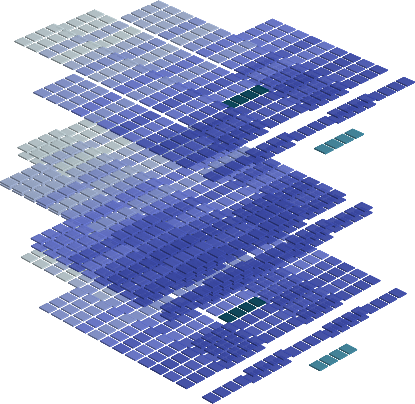
\includegraphics[width=1.5cm]{src/colorspace_colourflow/flows/colourflow_134-45.png}%           
  \end{adjustbox}                                                        
\caption*{

\begin{tikzpicture}                             
\definecolor{tempcolor}{HTML}{000000}           
\fill[tempcolor] (1 mm,0) rectangle ++(1mm,1mm);
\definecolor{tempcolor}{HTML}{4c5fd4}           
\fill[tempcolor] (2 mm,0) rectangle ++(1mm,1mm);
\definecolor{tempcolor}{HTML}{5d70e5}           
\fill[tempcolor] (3 mm,0) rectangle ++(1mm,1mm);
\definecolor{tempcolor}{HTML}{7f92ff}           
\fill[tempcolor] (4 mm,0) rectangle ++(1mm,1mm);
\definecolor{tempcolor}{HTML}{a1b4ff}           
\fill[tempcolor] (5 mm,0) rectangle ++(1mm,1mm);
\definecolor{tempcolor}{HTML}{c3d6ff}           
\fill[tempcolor] (6 mm,0) rectangle ++(1mm,1mm);
\definecolor{tempcolor}{HTML}{e5f8ff}           
\fill[tempcolor] (7 mm,0) rectangle ++(1mm,1mm);
\definecolor{tempcolor}{HTML}{001b63}           
\fill[tempcolor] (8 mm,0) rectangle ++(1mm,1mm);
\end{tikzpicture}                               
}
\end{figure}                                                               
\end{minipage}
\hspace{0.1cm}
\begin{minipage}[b]{0.15\linewidth}
\begin{figure}[H]                                                          
  \centering                                                             
  \begin{adjustbox}{width=1.5cm,center}                                   
  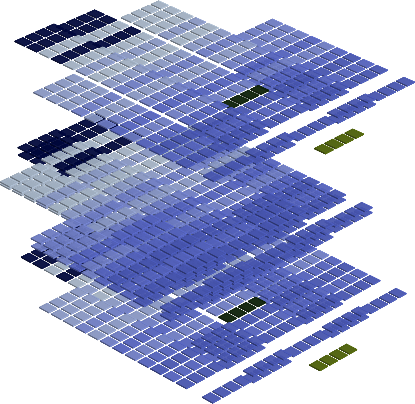
\includegraphics[width=1.5cm]{src/colorspace_colourflow/flows/colourflow_135-45.png}%           
  \end{adjustbox}                                                        
\caption*{

\begin{tikzpicture}                             
\definecolor{tempcolor}{HTML}{000000}           
\fill[tempcolor] (1 mm,0) rectangle ++(1mm,1mm);
\definecolor{tempcolor}{HTML}{5d70e5}           
\fill[tempcolor] (2 mm,0) rectangle ++(1mm,1mm);
\definecolor{tempcolor}{HTML}{6e81f6}           
\fill[tempcolor] (3 mm,0) rectangle ++(1mm,1mm);
\definecolor{tempcolor}{HTML}{90a3ff}           
\fill[tempcolor] (4 mm,0) rectangle ++(1mm,1mm);
\definecolor{tempcolor}{HTML}{b2c5ff}           
\fill[tempcolor] (5 mm,0) rectangle ++(1mm,1mm);
\definecolor{tempcolor}{HTML}{d4e7ff}           
\fill[tempcolor] (6 mm,0) rectangle ++(1mm,1mm);
\definecolor{tempcolor}{HTML}{000a4d}           
\fill[tempcolor] (7 mm,0) rectangle ++(1mm,1mm);
\definecolor{tempcolor}{HTML}{002c79}           
\fill[tempcolor] (8 mm,0) rectangle ++(1mm,1mm);
\end{tikzpicture}                               
}
\end{figure}                                                               
\end{minipage}
\hspace{0.1cm}
\begin{minipage}[b]{0.15\linewidth}
\begin{figure}[H]                                                          
  \centering                                                             
  \begin{adjustbox}{width=1.5cm,center}                                   
  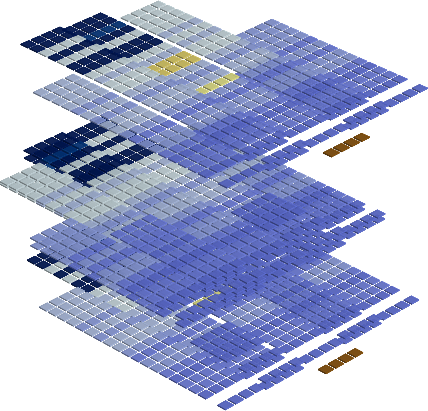
\includegraphics[width=1.5cm]{src/colorspace_colourflow/flows/colourflow_136-45.png}%           
  \end{adjustbox}                                                        
\caption*{

\begin{tikzpicture}                             
\definecolor{tempcolor}{HTML}{000000}           
\fill[tempcolor] (1 mm,0) rectangle ++(1mm,1mm);
\definecolor{tempcolor}{HTML}{6e81f6}           
\fill[tempcolor] (2 mm,0) rectangle ++(1mm,1mm);
\definecolor{tempcolor}{HTML}{7f92ff}           
\fill[tempcolor] (3 mm,0) rectangle ++(1mm,1mm);
\definecolor{tempcolor}{HTML}{a1b4ff}           
\fill[tempcolor] (4 mm,0) rectangle ++(1mm,1mm);
\definecolor{tempcolor}{HTML}{c3d6ff}           
\fill[tempcolor] (5 mm,0) rectangle ++(1mm,1mm);
\definecolor{tempcolor}{HTML}{e5f8ff}           
\fill[tempcolor] (6 mm,0) rectangle ++(1mm,1mm);
\definecolor{tempcolor}{HTML}{001b63}           
\fill[tempcolor] (7 mm,0) rectangle ++(1mm,1mm);
\definecolor{tempcolor}{HTML}{023d8f}           
\fill[tempcolor] (8 mm,0) rectangle ++(1mm,1mm);
\end{tikzpicture}                               
}
\end{figure}                                                               
\end{minipage}
\hspace{0.1cm}
\begin{minipage}[b]{0.15\linewidth}
\begin{figure}[H]                                                          
  \centering                                                             
  \begin{adjustbox}{width=1.5cm,center}                                   
  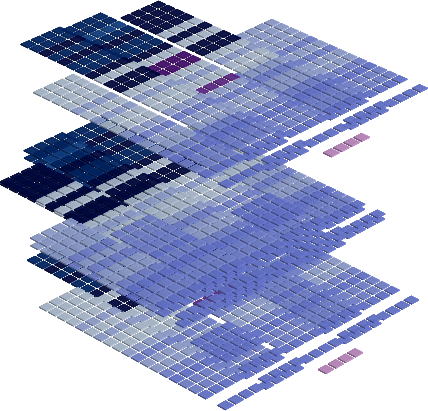
\includegraphics[width=1.5cm]{src/colorspace_colourflow/flows/colourflow_137-45.png}%           
  \end{adjustbox}                                                        
\caption*{

\begin{tikzpicture}                             
\definecolor{tempcolor}{HTML}{000000}           
\fill[tempcolor] (1 mm,0) rectangle ++(1mm,1mm);
\definecolor{tempcolor}{HTML}{7f92ff}           
\fill[tempcolor] (2 mm,0) rectangle ++(1mm,1mm);
\definecolor{tempcolor}{HTML}{90a3ff}           
\fill[tempcolor] (3 mm,0) rectangle ++(1mm,1mm);
\definecolor{tempcolor}{HTML}{b2c5ff}           
\fill[tempcolor] (4 mm,0) rectangle ++(1mm,1mm);
\definecolor{tempcolor}{HTML}{d4e7ff}           
\fill[tempcolor] (5 mm,0) rectangle ++(1mm,1mm);
\definecolor{tempcolor}{HTML}{000a4d}           
\fill[tempcolor] (6 mm,0) rectangle ++(1mm,1mm);
\definecolor{tempcolor}{HTML}{002c79}           
\fill[tempcolor] (7 mm,0) rectangle ++(1mm,1mm);
\definecolor{tempcolor}{HTML}{134ea0}           
\fill[tempcolor] (8 mm,0) rectangle ++(1mm,1mm);
\end{tikzpicture}                               
}
\end{figure}                                                               
\end{minipage}
\hspace{0.1cm}
\begin{minipage}[b]{0.15\linewidth}
\begin{figure}[H]                                                          
  \centering                                                             
  \begin{adjustbox}{width=1.5cm,center}                                   
  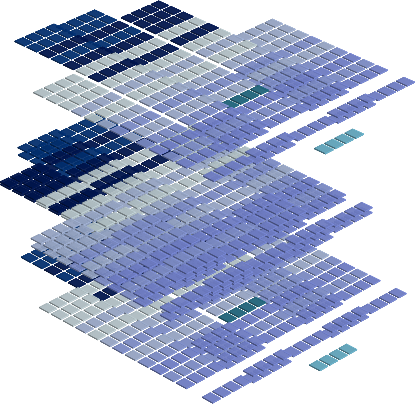
\includegraphics[width=1.5cm]{src/colorspace_colourflow/flows/colourflow_138-45.png}%           
  \end{adjustbox}                                                        
\caption*{

\begin{tikzpicture}                             
\definecolor{tempcolor}{HTML}{000000}           
\fill[tempcolor] (1 mm,0) rectangle ++(1mm,1mm);
\definecolor{tempcolor}{HTML}{90a3ff}           
\fill[tempcolor] (2 mm,0) rectangle ++(1mm,1mm);
\definecolor{tempcolor}{HTML}{a1b4ff}           
\fill[tempcolor] (3 mm,0) rectangle ++(1mm,1mm);
\definecolor{tempcolor}{HTML}{c3d6ff}           
\fill[tempcolor] (4 mm,0) rectangle ++(1mm,1mm);
\definecolor{tempcolor}{HTML}{e5f8ff}           
\fill[tempcolor] (5 mm,0) rectangle ++(1mm,1mm);
\definecolor{tempcolor}{HTML}{001b63}           
\fill[tempcolor] (6 mm,0) rectangle ++(1mm,1mm);
\definecolor{tempcolor}{HTML}{023d8f}           
\fill[tempcolor] (7 mm,0) rectangle ++(1mm,1mm);
\definecolor{tempcolor}{HTML}{245fb1}           
\fill[tempcolor] (8 mm,0) rectangle ++(1mm,1mm);
\end{tikzpicture}                               
}
\end{figure}                                                               
\end{minipage}
\hspace{0.1cm}
\begin{minipage}[b]{0.15\linewidth}
\begin{figure}[H]                                                          
  \centering                                                             
  \begin{adjustbox}{width=1.5cm,center}                                   
  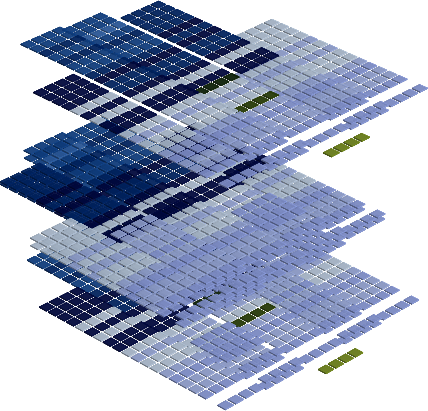
\includegraphics[width=1.5cm]{src/colorspace_colourflow/flows/colourflow_139-45.png}%           
  \end{adjustbox}                                                        
\caption*{

\begin{tikzpicture}                             
\definecolor{tempcolor}{HTML}{000000}           
\fill[tempcolor] (1 mm,0) rectangle ++(1mm,1mm);
\definecolor{tempcolor}{HTML}{a1b4ff}           
\fill[tempcolor] (2 mm,0) rectangle ++(1mm,1mm);
\definecolor{tempcolor}{HTML}{b2c5ff}           
\fill[tempcolor] (3 mm,0) rectangle ++(1mm,1mm);
\definecolor{tempcolor}{HTML}{d4e7ff}           
\fill[tempcolor] (4 mm,0) rectangle ++(1mm,1mm);
\definecolor{tempcolor}{HTML}{000a4d}           
\fill[tempcolor] (5 mm,0) rectangle ++(1mm,1mm);
\definecolor{tempcolor}{HTML}{002c79}           
\fill[tempcolor] (6 mm,0) rectangle ++(1mm,1mm);
\definecolor{tempcolor}{HTML}{134ea0}           
\fill[tempcolor] (7 mm,0) rectangle ++(1mm,1mm);
\definecolor{tempcolor}{HTML}{3570c2}           
\fill[tempcolor] (8 mm,0) rectangle ++(1mm,1mm);
\end{tikzpicture}                               
}
\end{figure}                                                               
\end{minipage}
\hspace{0.1cm}
\begin{minipage}[b]{0.15\linewidth}
\begin{figure}[H]                                                          
  \centering                                                             
  \begin{adjustbox}{width=1.5cm,center}                                   
  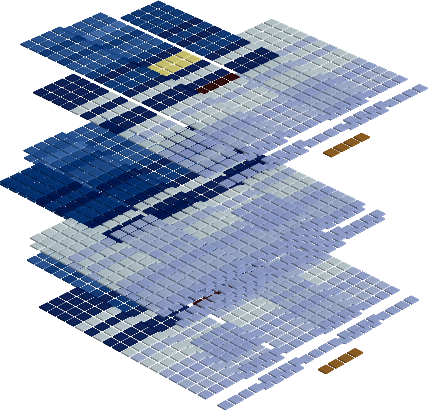
\includegraphics[width=1.5cm]{src/colorspace_colourflow/flows/colourflow_140-45.png}%           
  \end{adjustbox}                                                        
\caption*{

\begin{tikzpicture}                             
\definecolor{tempcolor}{HTML}{000000}           
\fill[tempcolor] (1 mm,0) rectangle ++(1mm,1mm);
\definecolor{tempcolor}{HTML}{b2c5ff}           
\fill[tempcolor] (2 mm,0) rectangle ++(1mm,1mm);
\definecolor{tempcolor}{HTML}{c3d6ff}           
\fill[tempcolor] (3 mm,0) rectangle ++(1mm,1mm);
\definecolor{tempcolor}{HTML}{e5f8ff}           
\fill[tempcolor] (4 mm,0) rectangle ++(1mm,1mm);
\definecolor{tempcolor}{HTML}{001b63}           
\fill[tempcolor] (5 mm,0) rectangle ++(1mm,1mm);
\definecolor{tempcolor}{HTML}{023d8f}           
\fill[tempcolor] (6 mm,0) rectangle ++(1mm,1mm);
\definecolor{tempcolor}{HTML}{245fb1}           
\fill[tempcolor] (7 mm,0) rectangle ++(1mm,1mm);
\definecolor{tempcolor}{HTML}{4681d3}           
\fill[tempcolor] (8 mm,0) rectangle ++(1mm,1mm);
\end{tikzpicture}                               
}
\end{figure}                                                               
\end{minipage}
\hspace{0.1cm}
\begin{minipage}[b]{0.15\linewidth}
\begin{figure}[H]                                                          
  \centering                                                             
  \begin{adjustbox}{width=1.5cm,center}                                   
  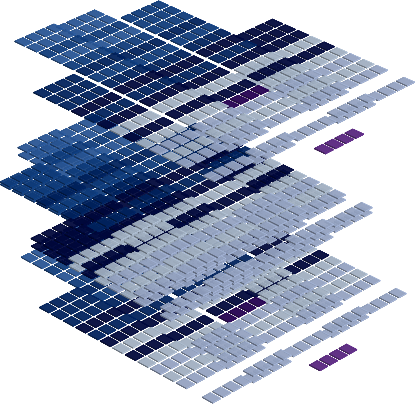
\includegraphics[width=1.5cm]{src/colorspace_colourflow/flows/colourflow_141-45.png}%           
  \end{adjustbox}                                                        
\caption*{

\begin{tikzpicture}                             
\definecolor{tempcolor}{HTML}{000000}           
\fill[tempcolor] (1 mm,0) rectangle ++(1mm,1mm);
\definecolor{tempcolor}{HTML}{c3d6ff}           
\fill[tempcolor] (2 mm,0) rectangle ++(1mm,1mm);
\definecolor{tempcolor}{HTML}{d4e7ff}           
\fill[tempcolor] (3 mm,0) rectangle ++(1mm,1mm);
\definecolor{tempcolor}{HTML}{000a4d}           
\fill[tempcolor] (4 mm,0) rectangle ++(1mm,1mm);
\definecolor{tempcolor}{HTML}{002c79}           
\fill[tempcolor] (5 mm,0) rectangle ++(1mm,1mm);
\definecolor{tempcolor}{HTML}{134ea0}           
\fill[tempcolor] (6 mm,0) rectangle ++(1mm,1mm);
\definecolor{tempcolor}{HTML}{3570c2}           
\fill[tempcolor] (7 mm,0) rectangle ++(1mm,1mm);
\definecolor{tempcolor}{HTML}{5792e4}           
\fill[tempcolor] (8 mm,0) rectangle ++(1mm,1mm);
\end{tikzpicture}                               
}
\end{figure}                                                               
\end{minipage}
\hspace{0.1cm}
\begin{minipage}[b]{0.15\linewidth}
\begin{figure}[H]                                                          
  \centering                                                             
  \begin{adjustbox}{width=1.5cm,center}                                   
  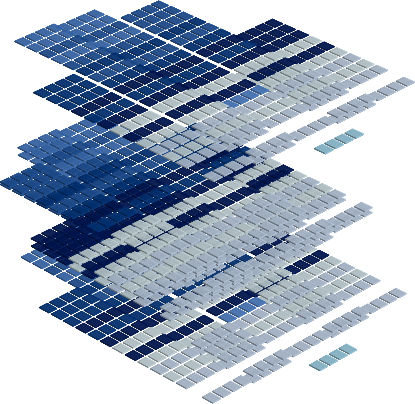
\includegraphics[width=1.5cm]{src/colorspace_colourflow/flows/colourflow_142-45.png}%           
  \end{adjustbox}                                                        
\caption*{

\begin{tikzpicture}                             
\definecolor{tempcolor}{HTML}{000000}           
\fill[tempcolor] (1 mm,0) rectangle ++(1mm,1mm);
\definecolor{tempcolor}{HTML}{d4e7ff}           
\fill[tempcolor] (2 mm,0) rectangle ++(1mm,1mm);
\definecolor{tempcolor}{HTML}{e5f8ff}           
\fill[tempcolor] (3 mm,0) rectangle ++(1mm,1mm);
\definecolor{tempcolor}{HTML}{001b63}           
\fill[tempcolor] (4 mm,0) rectangle ++(1mm,1mm);
\definecolor{tempcolor}{HTML}{023d8f}           
\fill[tempcolor] (5 mm,0) rectangle ++(1mm,1mm);
\definecolor{tempcolor}{HTML}{245fb1}           
\fill[tempcolor] (6 mm,0) rectangle ++(1mm,1mm);
\definecolor{tempcolor}{HTML}{4681d3}           
\fill[tempcolor] (7 mm,0) rectangle ++(1mm,1mm);
\definecolor{tempcolor}{HTML}{68a3f5}           
\fill[tempcolor] (8 mm,0) rectangle ++(1mm,1mm);
\end{tikzpicture}                               
}
\end{figure}                                                               
\end{minipage}
\hspace{0.1cm}
\begin{minipage}[b]{0.15\linewidth}
\begin{figure}[H]                                                          
  \centering                                                             
  \begin{adjustbox}{width=1.5cm,center}                                   
  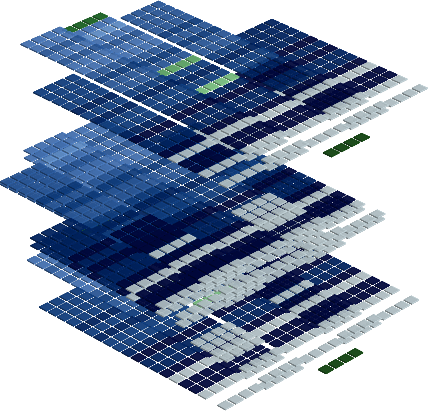
\includegraphics[width=1.5cm]{src/colorspace_colourflow/flows/colourflow_143-45.png}%           
  \end{adjustbox}                                                        
\caption*{

\begin{tikzpicture}                             
\definecolor{tempcolor}{HTML}{000000}           
\fill[tempcolor] (1 mm,0) rectangle ++(1mm,1mm);
\definecolor{tempcolor}{HTML}{e5f8ff}           
\fill[tempcolor] (2 mm,0) rectangle ++(1mm,1mm);
\definecolor{tempcolor}{HTML}{000a4d}           
\fill[tempcolor] (3 mm,0) rectangle ++(1mm,1mm);
\definecolor{tempcolor}{HTML}{002c79}           
\fill[tempcolor] (4 mm,0) rectangle ++(1mm,1mm);
\definecolor{tempcolor}{HTML}{134ea0}           
\fill[tempcolor] (5 mm,0) rectangle ++(1mm,1mm);
\definecolor{tempcolor}{HTML}{3570c2}           
\fill[tempcolor] (6 mm,0) rectangle ++(1mm,1mm);
\definecolor{tempcolor}{HTML}{5792e4}           
\fill[tempcolor] (7 mm,0) rectangle ++(1mm,1mm);
\definecolor{tempcolor}{HTML}{79b4ff}           
\fill[tempcolor] (8 mm,0) rectangle ++(1mm,1mm);
\end{tikzpicture}                               
}
\end{figure}                                                               
\end{minipage}
\hspace{0.1cm}
\begin{minipage}[b]{0.15\linewidth}
\begin{figure}[H]                                                          
  \centering                                                             
  \begin{adjustbox}{width=1.5cm,center}                                   
  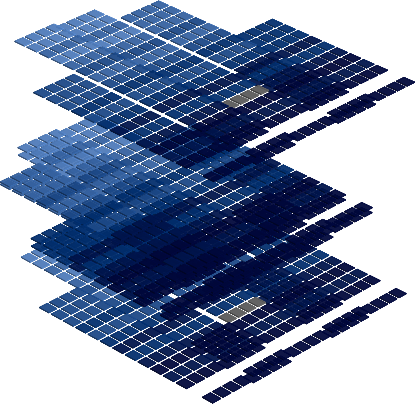
\includegraphics[width=1.5cm]{src/colorspace_colourflow/flows/colourflow_144-45.png}%           
  \end{adjustbox}                                                        
\caption*{

\begin{tikzpicture}                             
\definecolor{tempcolor}{HTML}{000000}           
\fill[tempcolor] (1 mm,0) rectangle ++(1mm,1mm);
\definecolor{tempcolor}{HTML}{000a4d}           
\fill[tempcolor] (2 mm,0) rectangle ++(1mm,1mm);
\definecolor{tempcolor}{HTML}{001b63}           
\fill[tempcolor] (3 mm,0) rectangle ++(1mm,1mm);
\definecolor{tempcolor}{HTML}{023d8f}           
\fill[tempcolor] (4 mm,0) rectangle ++(1mm,1mm);
\definecolor{tempcolor}{HTML}{245fb1}           
\fill[tempcolor] (5 mm,0) rectangle ++(1mm,1mm);
\definecolor{tempcolor}{HTML}{4681d3}           
\fill[tempcolor] (6 mm,0) rectangle ++(1mm,1mm);
\definecolor{tempcolor}{HTML}{68a3f5}           
\fill[tempcolor] (7 mm,0) rectangle ++(1mm,1mm);
\definecolor{tempcolor}{HTML}{8ac5ff}           
\fill[tempcolor] (8 mm,0) rectangle ++(1mm,1mm);
\end{tikzpicture}                               
}
\end{figure}                                                               
\end{minipage}
\hspace{0.1cm}
\begin{minipage}[b]{0.15\linewidth}
\begin{figure}[H]                                                          
  \centering                                                             
  \begin{adjustbox}{width=1.5cm,center}                                   
  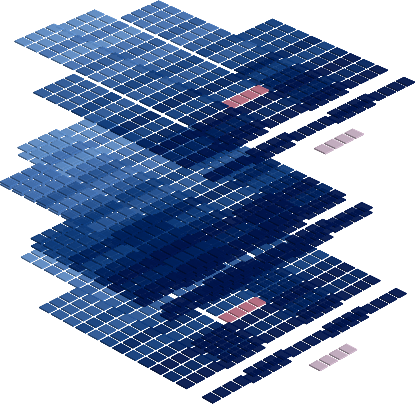
\includegraphics[width=1.5cm]{src/colorspace_colourflow/flows/colourflow_145-45.png}%           
  \end{adjustbox}                                                        
\caption*{

\begin{tikzpicture}                             
\definecolor{tempcolor}{HTML}{000000}           
\fill[tempcolor] (1 mm,0) rectangle ++(1mm,1mm);
\definecolor{tempcolor}{HTML}{001b63}           
\fill[tempcolor] (2 mm,0) rectangle ++(1mm,1mm);
\definecolor{tempcolor}{HTML}{002c79}           
\fill[tempcolor] (3 mm,0) rectangle ++(1mm,1mm);
\definecolor{tempcolor}{HTML}{134ea0}           
\fill[tempcolor] (4 mm,0) rectangle ++(1mm,1mm);
\definecolor{tempcolor}{HTML}{3570c2}           
\fill[tempcolor] (5 mm,0) rectangle ++(1mm,1mm);
\definecolor{tempcolor}{HTML}{5792e4}           
\fill[tempcolor] (6 mm,0) rectangle ++(1mm,1mm);
\definecolor{tempcolor}{HTML}{79b4ff}           
\fill[tempcolor] (7 mm,0) rectangle ++(1mm,1mm);
\definecolor{tempcolor}{HTML}{9bd6ff}           
\fill[tempcolor] (8 mm,0) rectangle ++(1mm,1mm);
\end{tikzpicture}                               
}
\end{figure}                                                               
\end{minipage}
\hspace{0.1cm}
\begin{minipage}[b]{0.15\linewidth}
\begin{figure}[H]                                                          
  \centering                                                             
  \begin{adjustbox}{width=1.5cm,center}                                   
  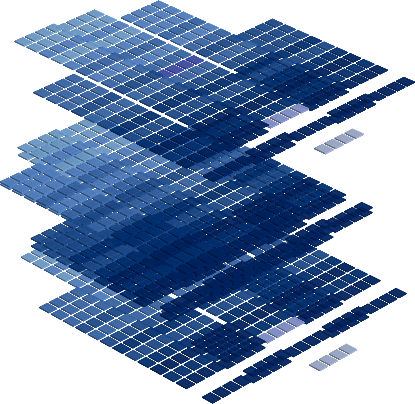
\includegraphics[width=1.5cm]{src/colorspace_colourflow/flows/colourflow_146-45.png}%           
  \end{adjustbox}                                                        
\caption*{

\begin{tikzpicture}                             
\definecolor{tempcolor}{HTML}{000000}           
\fill[tempcolor] (1 mm,0) rectangle ++(1mm,1mm);
\definecolor{tempcolor}{HTML}{002c79}           
\fill[tempcolor] (2 mm,0) rectangle ++(1mm,1mm);
\definecolor{tempcolor}{HTML}{023d8f}           
\fill[tempcolor] (3 mm,0) rectangle ++(1mm,1mm);
\definecolor{tempcolor}{HTML}{245fb1}           
\fill[tempcolor] (4 mm,0) rectangle ++(1mm,1mm);
\definecolor{tempcolor}{HTML}{4681d3}           
\fill[tempcolor] (5 mm,0) rectangle ++(1mm,1mm);
\definecolor{tempcolor}{HTML}{68a3f5}           
\fill[tempcolor] (6 mm,0) rectangle ++(1mm,1mm);
\definecolor{tempcolor}{HTML}{8ac5ff}           
\fill[tempcolor] (7 mm,0) rectangle ++(1mm,1mm);
\definecolor{tempcolor}{HTML}{ace7ff}           
\fill[tempcolor] (8 mm,0) rectangle ++(1mm,1mm);
\end{tikzpicture}                               
}
\end{figure}                                                               
\end{minipage}
\hspace{0.1cm}
\begin{minipage}[b]{0.15\linewidth}
\begin{figure}[H]                                                          
  \centering                                                             
  \begin{adjustbox}{width=1.5cm,center}                                   
  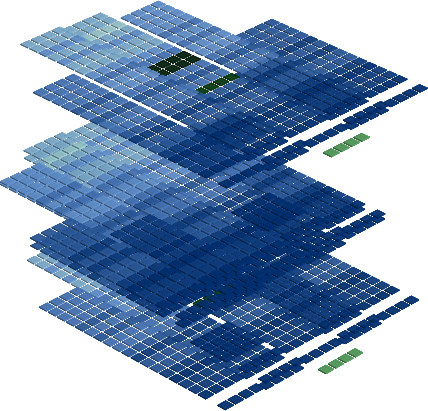
\includegraphics[width=1.5cm]{src/colorspace_colourflow/flows/colourflow_147-45.png}%           
  \end{adjustbox}                                                        
\caption*{

\begin{tikzpicture}                             
\definecolor{tempcolor}{HTML}{000000}           
\fill[tempcolor] (1 mm,0) rectangle ++(1mm,1mm);
\definecolor{tempcolor}{HTML}{023d8f}           
\fill[tempcolor] (2 mm,0) rectangle ++(1mm,1mm);
\definecolor{tempcolor}{HTML}{134ea0}           
\fill[tempcolor] (3 mm,0) rectangle ++(1mm,1mm);
\definecolor{tempcolor}{HTML}{3570c2}           
\fill[tempcolor] (4 mm,0) rectangle ++(1mm,1mm);
\definecolor{tempcolor}{HTML}{5792e4}           
\fill[tempcolor] (5 mm,0) rectangle ++(1mm,1mm);
\definecolor{tempcolor}{HTML}{79b4ff}           
\fill[tempcolor] (6 mm,0) rectangle ++(1mm,1mm);
\definecolor{tempcolor}{HTML}{9bd6ff}           
\fill[tempcolor] (7 mm,0) rectangle ++(1mm,1mm);
\definecolor{tempcolor}{HTML}{bdf8ff}           
\fill[tempcolor] (8 mm,0) rectangle ++(1mm,1mm);
\end{tikzpicture}                               
}
\end{figure}                                                               
\end{minipage}
\hspace{0.1cm}
\begin{minipage}[b]{0.15\linewidth}
\begin{figure}[H]                                                          
  \centering                                                             
  \begin{adjustbox}{width=1.5cm,center}                                   
  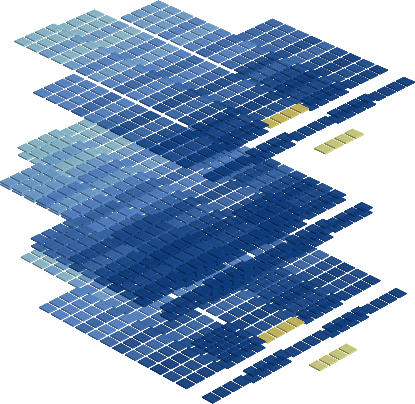
\includegraphics[width=1.5cm]{src/colorspace_colourflow/flows/colourflow_148-45.png}%           
  \end{adjustbox}                                                        
\caption*{

\begin{tikzpicture}                             
\definecolor{tempcolor}{HTML}{000000}           
\fill[tempcolor] (1 mm,0) rectangle ++(1mm,1mm);
\definecolor{tempcolor}{HTML}{134ea0}           
\fill[tempcolor] (2 mm,0) rectangle ++(1mm,1mm);
\definecolor{tempcolor}{HTML}{245fb1}           
\fill[tempcolor] (3 mm,0) rectangle ++(1mm,1mm);
\definecolor{tempcolor}{HTML}{4681d3}           
\fill[tempcolor] (4 mm,0) rectangle ++(1mm,1mm);
\definecolor{tempcolor}{HTML}{68a3f5}           
\fill[tempcolor] (5 mm,0) rectangle ++(1mm,1mm);
\definecolor{tempcolor}{HTML}{8ac5ff}           
\fill[tempcolor] (6 mm,0) rectangle ++(1mm,1mm);
\definecolor{tempcolor}{HTML}{ace7ff}           
\fill[tempcolor] (7 mm,0) rectangle ++(1mm,1mm);
\definecolor{tempcolor}{HTML}{ceffff}           
\fill[tempcolor] (8 mm,0) rectangle ++(1mm,1mm);
\end{tikzpicture}                               
}
\end{figure}                                                               
\end{minipage}
\hspace{0.1cm}
\begin{minipage}[b]{0.15\linewidth}
\begin{figure}[H]                                                          
  \centering                                                             
  \begin{adjustbox}{width=1.5cm,center}                                   
  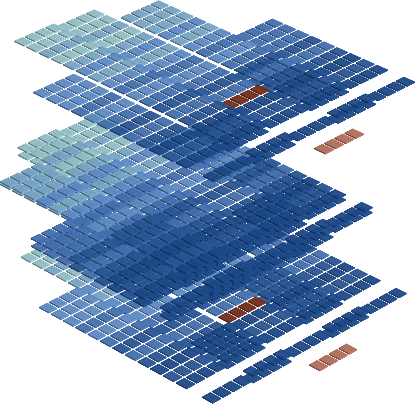
\includegraphics[width=1.5cm]{src/colorspace_colourflow/flows/colourflow_149-45.png}%           
  \end{adjustbox}                                                        
\caption*{

\begin{tikzpicture}                             
\definecolor{tempcolor}{HTML}{000000}           
\fill[tempcolor] (1 mm,0) rectangle ++(1mm,1mm);
\definecolor{tempcolor}{HTML}{245fb1}           
\fill[tempcolor] (2 mm,0) rectangle ++(1mm,1mm);
\definecolor{tempcolor}{HTML}{3570c2}           
\fill[tempcolor] (3 mm,0) rectangle ++(1mm,1mm);
\definecolor{tempcolor}{HTML}{5792e4}           
\fill[tempcolor] (4 mm,0) rectangle ++(1mm,1mm);
\definecolor{tempcolor}{HTML}{79b4ff}           
\fill[tempcolor] (5 mm,0) rectangle ++(1mm,1mm);
\definecolor{tempcolor}{HTML}{9bd6ff}           
\fill[tempcolor] (6 mm,0) rectangle ++(1mm,1mm);
\definecolor{tempcolor}{HTML}{bdf8ff}           
\fill[tempcolor] (7 mm,0) rectangle ++(1mm,1mm);
\definecolor{tempcolor}{HTML}{001a26}           
\fill[tempcolor] (8 mm,0) rectangle ++(1mm,1mm);
\end{tikzpicture}                               
}
\end{figure}                                                               
\end{minipage}
\hspace{0.1cm}
\begin{minipage}[b]{0.15\linewidth}
\begin{figure}[H]                                                          
  \centering                                                             
  \begin{adjustbox}{width=1.5cm,center}                                   
  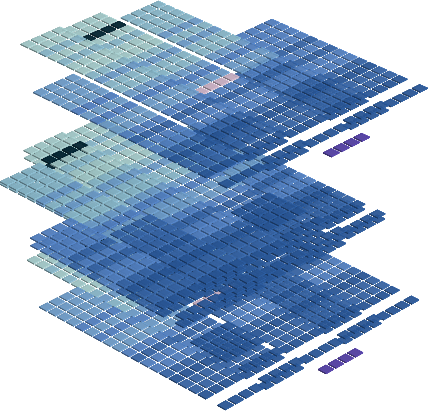
\includegraphics[width=1.5cm]{src/colorspace_colourflow/flows/colourflow_150-45.png}%           
  \end{adjustbox}                                                        
\caption*{

\begin{tikzpicture}                             
\definecolor{tempcolor}{HTML}{000000}           
\fill[tempcolor] (1 mm,0) rectangle ++(1mm,1mm);
\definecolor{tempcolor}{HTML}{3570c2}           
\fill[tempcolor] (2 mm,0) rectangle ++(1mm,1mm);
\definecolor{tempcolor}{HTML}{4681d3}           
\fill[tempcolor] (3 mm,0) rectangle ++(1mm,1mm);
\definecolor{tempcolor}{HTML}{68a3f5}           
\fill[tempcolor] (4 mm,0) rectangle ++(1mm,1mm);
\definecolor{tempcolor}{HTML}{8ac5ff}           
\fill[tempcolor] (5 mm,0) rectangle ++(1mm,1mm);
\definecolor{tempcolor}{HTML}{ace7ff}           
\fill[tempcolor] (6 mm,0) rectangle ++(1mm,1mm);
\definecolor{tempcolor}{HTML}{ceffff}           
\fill[tempcolor] (7 mm,0) rectangle ++(1mm,1mm);
\definecolor{tempcolor}{HTML}{002b3c}           
\fill[tempcolor] (8 mm,0) rectangle ++(1mm,1mm);
\end{tikzpicture}                               
}
\end{figure}                                                               
\end{minipage}
\hspace{0.1cm}
\begin{minipage}[b]{0.15\linewidth}
\begin{figure}[H]                                                          
  \centering                                                             
  \begin{adjustbox}{width=1.5cm,center}                                   
  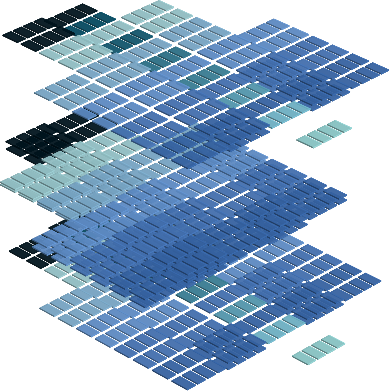
\includegraphics[width=1.5cm]{src/colorspace_colourflow/flows/colourflow_151-45.png}%           
  \end{adjustbox}                                                        
\caption*{

\begin{tikzpicture}                             
\definecolor{tempcolor}{HTML}{000000}           
\fill[tempcolor] (1 mm,0) rectangle ++(1mm,1mm);
\definecolor{tempcolor}{HTML}{4681d3}           
\fill[tempcolor] (2 mm,0) rectangle ++(1mm,1mm);
\definecolor{tempcolor}{HTML}{5792e4}           
\fill[tempcolor] (3 mm,0) rectangle ++(1mm,1mm);
\definecolor{tempcolor}{HTML}{79b4ff}           
\fill[tempcolor] (4 mm,0) rectangle ++(1mm,1mm);
\definecolor{tempcolor}{HTML}{9bd6ff}           
\fill[tempcolor] (5 mm,0) rectangle ++(1mm,1mm);
\definecolor{tempcolor}{HTML}{bdf8ff}           
\fill[tempcolor] (6 mm,0) rectangle ++(1mm,1mm);
\definecolor{tempcolor}{HTML}{001a26}           
\fill[tempcolor] (7 mm,0) rectangle ++(1mm,1mm);
\definecolor{tempcolor}{HTML}{003c52}           
\fill[tempcolor] (8 mm,0) rectangle ++(1mm,1mm);
\end{tikzpicture}                               
}
\end{figure}                                                               
\end{minipage}
\hspace{0.1cm}
\begin{minipage}[b]{0.15\linewidth}
\begin{figure}[H]                                                          
  \centering                                                             
  \begin{adjustbox}{width=1.5cm,center}                                   
  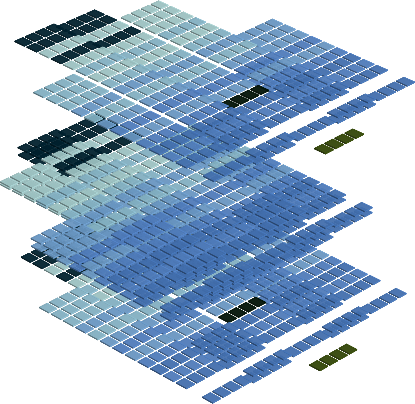
\includegraphics[width=1.5cm]{src/colorspace_colourflow/flows/colourflow_152-45.png}%           
  \end{adjustbox}                                                        
\caption*{

\begin{tikzpicture}                             
\definecolor{tempcolor}{HTML}{000000}           
\fill[tempcolor] (1 mm,0) rectangle ++(1mm,1mm);
\definecolor{tempcolor}{HTML}{5792e4}           
\fill[tempcolor] (2 mm,0) rectangle ++(1mm,1mm);
\definecolor{tempcolor}{HTML}{68a3f5}           
\fill[tempcolor] (3 mm,0) rectangle ++(1mm,1mm);
\definecolor{tempcolor}{HTML}{8ac5ff}           
\fill[tempcolor] (4 mm,0) rectangle ++(1mm,1mm);
\definecolor{tempcolor}{HTML}{ace7ff}           
\fill[tempcolor] (5 mm,0) rectangle ++(1mm,1mm);
\definecolor{tempcolor}{HTML}{ceffff}           
\fill[tempcolor] (6 mm,0) rectangle ++(1mm,1mm);
\definecolor{tempcolor}{HTML}{002b3c}           
\fill[tempcolor] (7 mm,0) rectangle ++(1mm,1mm);
\definecolor{tempcolor}{HTML}{004d68}           
\fill[tempcolor] (8 mm,0) rectangle ++(1mm,1mm);
\end{tikzpicture}                               
}
\end{figure}                                                               
\end{minipage}
\hspace{0.1cm}
\begin{minipage}[b]{0.15\linewidth}
\begin{figure}[H]                                                          
  \centering                                                             
  \begin{adjustbox}{width=1.5cm,center}                                   
  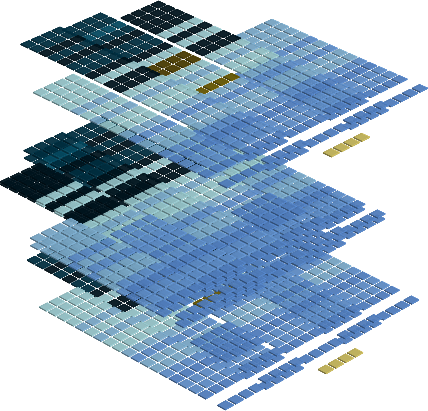
\includegraphics[width=1.5cm]{src/colorspace_colourflow/flows/colourflow_153-45.png}%           
  \end{adjustbox}                                                        
\caption*{

\begin{tikzpicture}                             
\definecolor{tempcolor}{HTML}{000000}           
\fill[tempcolor] (1 mm,0) rectangle ++(1mm,1mm);
\definecolor{tempcolor}{HTML}{68a3f5}           
\fill[tempcolor] (2 mm,0) rectangle ++(1mm,1mm);
\definecolor{tempcolor}{HTML}{79b4ff}           
\fill[tempcolor] (3 mm,0) rectangle ++(1mm,1mm);
\definecolor{tempcolor}{HTML}{9bd6ff}           
\fill[tempcolor] (4 mm,0) rectangle ++(1mm,1mm);
\definecolor{tempcolor}{HTML}{bdf8ff}           
\fill[tempcolor] (5 mm,0) rectangle ++(1mm,1mm);
\definecolor{tempcolor}{HTML}{001a26}           
\fill[tempcolor] (6 mm,0) rectangle ++(1mm,1mm);
\definecolor{tempcolor}{HTML}{003c52}           
\fill[tempcolor] (7 mm,0) rectangle ++(1mm,1mm);
\definecolor{tempcolor}{HTML}{065e7c}           
\fill[tempcolor] (8 mm,0) rectangle ++(1mm,1mm);
\end{tikzpicture}                               
}
\end{figure}                                                               
\end{minipage}
\hspace{0.1cm}
\begin{minipage}[b]{0.15\linewidth}
\begin{figure}[H]                                                          
  \centering                                                             
  \begin{adjustbox}{width=1.5cm,center}                                   
  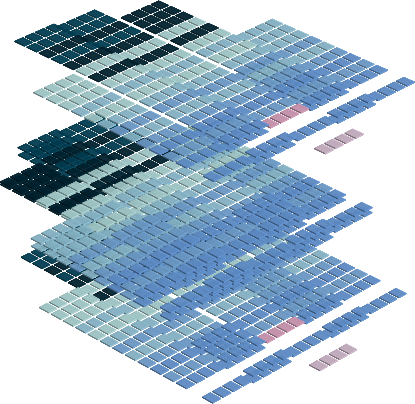
\includegraphics[width=1.5cm]{src/colorspace_colourflow/flows/colourflow_154-45.png}%           
  \end{adjustbox}                                                        
\caption*{

\begin{tikzpicture}                             
\definecolor{tempcolor}{HTML}{000000}           
\fill[tempcolor] (1 mm,0) rectangle ++(1mm,1mm);
\definecolor{tempcolor}{HTML}{79b4ff}           
\fill[tempcolor] (2 mm,0) rectangle ++(1mm,1mm);
\definecolor{tempcolor}{HTML}{8ac5ff}           
\fill[tempcolor] (3 mm,0) rectangle ++(1mm,1mm);
\definecolor{tempcolor}{HTML}{ace7ff}           
\fill[tempcolor] (4 mm,0) rectangle ++(1mm,1mm);
\definecolor{tempcolor}{HTML}{ceffff}           
\fill[tempcolor] (5 mm,0) rectangle ++(1mm,1mm);
\definecolor{tempcolor}{HTML}{002b3c}           
\fill[tempcolor] (6 mm,0) rectangle ++(1mm,1mm);
\definecolor{tempcolor}{HTML}{004d68}           
\fill[tempcolor] (7 mm,0) rectangle ++(1mm,1mm);
\definecolor{tempcolor}{HTML}{176f8d}           
\fill[tempcolor] (8 mm,0) rectangle ++(1mm,1mm);
\end{tikzpicture}                               
}
\end{figure}                                                               
\end{minipage}
\hspace{0.1cm}
\begin{minipage}[b]{0.15\linewidth}
\begin{figure}[H]                                                          
  \centering                                                             
  \begin{adjustbox}{width=1.5cm,center}                                   
  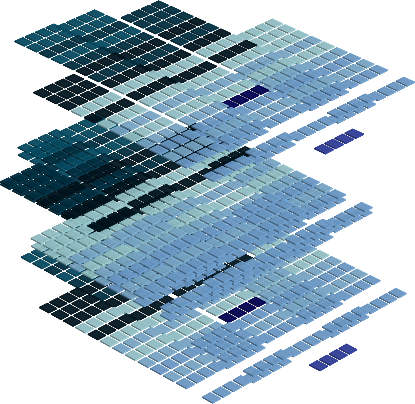
\includegraphics[width=1.5cm]{src/colorspace_colourflow/flows/colourflow_155-45.png}%           
  \end{adjustbox}                                                        
\caption*{

\begin{tikzpicture}                             
\definecolor{tempcolor}{HTML}{000000}           
\fill[tempcolor] (1 mm,0) rectangle ++(1mm,1mm);
\definecolor{tempcolor}{HTML}{8ac5ff}           
\fill[tempcolor] (2 mm,0) rectangle ++(1mm,1mm);
\definecolor{tempcolor}{HTML}{9bd6ff}           
\fill[tempcolor] (3 mm,0) rectangle ++(1mm,1mm);
\definecolor{tempcolor}{HTML}{bdf8ff}           
\fill[tempcolor] (4 mm,0) rectangle ++(1mm,1mm);
\definecolor{tempcolor}{HTML}{001a26}           
\fill[tempcolor] (5 mm,0) rectangle ++(1mm,1mm);
\definecolor{tempcolor}{HTML}{003c52}           
\fill[tempcolor] (6 mm,0) rectangle ++(1mm,1mm);
\definecolor{tempcolor}{HTML}{065e7c}           
\fill[tempcolor] (7 mm,0) rectangle ++(1mm,1mm);
\definecolor{tempcolor}{HTML}{28809e}           
\fill[tempcolor] (8 mm,0) rectangle ++(1mm,1mm);
\end{tikzpicture}                               
}
\end{figure}                                                               
\end{minipage}
\hspace{0.1cm}
\begin{minipage}[b]{0.15\linewidth}
\begin{figure}[H]                                                          
  \centering                                                             
  \begin{adjustbox}{width=1.5cm,center}                                   
  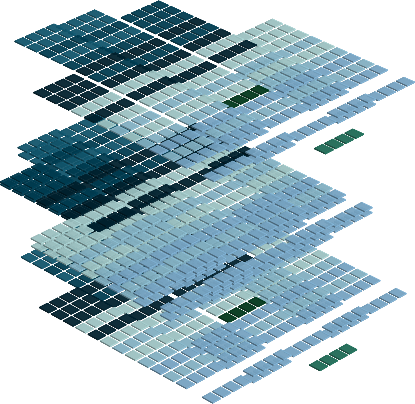
\includegraphics[width=1.5cm]{src/colorspace_colourflow/flows/colourflow_156-45.png}%           
  \end{adjustbox}                                                        
\caption*{

\begin{tikzpicture}                             
\definecolor{tempcolor}{HTML}{000000}           
\fill[tempcolor] (1 mm,0) rectangle ++(1mm,1mm);
\definecolor{tempcolor}{HTML}{9bd6ff}           
\fill[tempcolor] (2 mm,0) rectangle ++(1mm,1mm);
\definecolor{tempcolor}{HTML}{ace7ff}           
\fill[tempcolor] (3 mm,0) rectangle ++(1mm,1mm);
\definecolor{tempcolor}{HTML}{ceffff}           
\fill[tempcolor] (4 mm,0) rectangle ++(1mm,1mm);
\definecolor{tempcolor}{HTML}{002b3c}           
\fill[tempcolor] (5 mm,0) rectangle ++(1mm,1mm);
\definecolor{tempcolor}{HTML}{004d68}           
\fill[tempcolor] (6 mm,0) rectangle ++(1mm,1mm);
\definecolor{tempcolor}{HTML}{176f8d}           
\fill[tempcolor] (7 mm,0) rectangle ++(1mm,1mm);
\definecolor{tempcolor}{HTML}{3991af}           
\fill[tempcolor] (8 mm,0) rectangle ++(1mm,1mm);
\end{tikzpicture}                               
}
\end{figure}                                                               
\end{minipage}
\hspace{0.1cm}
\begin{minipage}[b]{0.15\linewidth}
\begin{figure}[H]                                                          
  \centering                                                             
  \begin{adjustbox}{width=1.5cm,center}                                   
  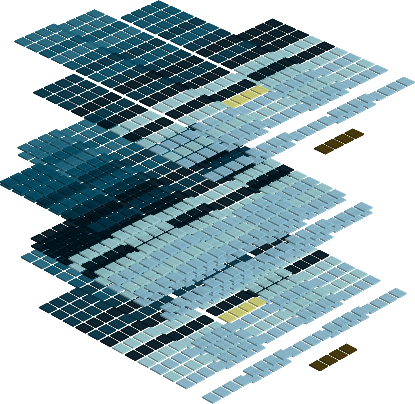
\includegraphics[width=1.5cm]{src/colorspace_colourflow/flows/colourflow_157-45.png}%           
  \end{adjustbox}                                                        
\caption*{

\begin{tikzpicture}                             
\definecolor{tempcolor}{HTML}{000000}           
\fill[tempcolor] (1 mm,0) rectangle ++(1mm,1mm);
\definecolor{tempcolor}{HTML}{ace7ff}           
\fill[tempcolor] (2 mm,0) rectangle ++(1mm,1mm);
\definecolor{tempcolor}{HTML}{bdf8ff}           
\fill[tempcolor] (3 mm,0) rectangle ++(1mm,1mm);
\definecolor{tempcolor}{HTML}{001a26}           
\fill[tempcolor] (4 mm,0) rectangle ++(1mm,1mm);
\definecolor{tempcolor}{HTML}{003c52}           
\fill[tempcolor] (5 mm,0) rectangle ++(1mm,1mm);
\definecolor{tempcolor}{HTML}{065e7c}           
\fill[tempcolor] (6 mm,0) rectangle ++(1mm,1mm);
\definecolor{tempcolor}{HTML}{28809e}           
\fill[tempcolor] (7 mm,0) rectangle ++(1mm,1mm);
\definecolor{tempcolor}{HTML}{4aa2c0}           
\fill[tempcolor] (8 mm,0) rectangle ++(1mm,1mm);
\end{tikzpicture}                               
}
\end{figure}                                                               
\end{minipage}
\hspace{0.1cm}
\begin{minipage}[b]{0.15\linewidth}
\begin{figure}[H]                                                          
  \centering                                                             
  \begin{adjustbox}{width=1.5cm,center}                                   
  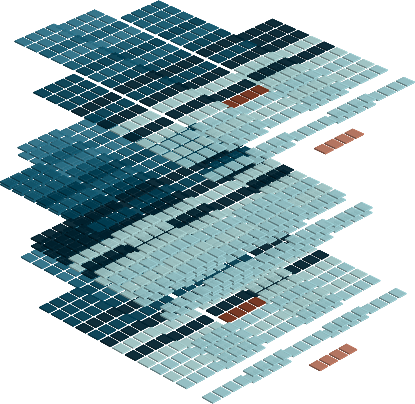
\includegraphics[width=1.5cm]{src/colorspace_colourflow/flows/colourflow_158-45.png}%           
  \end{adjustbox}                                                        
\caption*{

\begin{tikzpicture}                             
\definecolor{tempcolor}{HTML}{000000}           
\fill[tempcolor] (1 mm,0) rectangle ++(1mm,1mm);
\definecolor{tempcolor}{HTML}{bdf8ff}           
\fill[tempcolor] (2 mm,0) rectangle ++(1mm,1mm);
\definecolor{tempcolor}{HTML}{ceffff}           
\fill[tempcolor] (3 mm,0) rectangle ++(1mm,1mm);
\definecolor{tempcolor}{HTML}{002b3c}           
\fill[tempcolor] (4 mm,0) rectangle ++(1mm,1mm);
\definecolor{tempcolor}{HTML}{004d68}           
\fill[tempcolor] (5 mm,0) rectangle ++(1mm,1mm);
\definecolor{tempcolor}{HTML}{176f8d}           
\fill[tempcolor] (6 mm,0) rectangle ++(1mm,1mm);
\definecolor{tempcolor}{HTML}{3991af}           
\fill[tempcolor] (7 mm,0) rectangle ++(1mm,1mm);
\definecolor{tempcolor}{HTML}{5bb3d1}           
\fill[tempcolor] (8 mm,0) rectangle ++(1mm,1mm);
\end{tikzpicture}                               
}
\end{figure}                                                               
\end{minipage}
\hspace{0.1cm}
\begin{minipage}[b]{0.15\linewidth}
\begin{figure}[H]                                                          
  \centering                                                             
  \begin{adjustbox}{width=1.5cm,center}                                   
  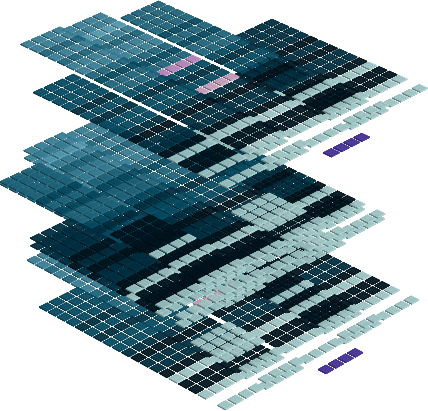
\includegraphics[width=1.5cm]{src/colorspace_colourflow/flows/colourflow_159-45.png}%           
  \end{adjustbox}                                                        
\caption*{

\begin{tikzpicture}                             
\definecolor{tempcolor}{HTML}{000000}           
\fill[tempcolor] (1 mm,0) rectangle ++(1mm,1mm);
\definecolor{tempcolor}{HTML}{ceffff}           
\fill[tempcolor] (2 mm,0) rectangle ++(1mm,1mm);
\definecolor{tempcolor}{HTML}{001a26}           
\fill[tempcolor] (3 mm,0) rectangle ++(1mm,1mm);
\definecolor{tempcolor}{HTML}{003c52}           
\fill[tempcolor] (4 mm,0) rectangle ++(1mm,1mm);
\definecolor{tempcolor}{HTML}{065e7c}           
\fill[tempcolor] (5 mm,0) rectangle ++(1mm,1mm);
\definecolor{tempcolor}{HTML}{28809e}           
\fill[tempcolor] (6 mm,0) rectangle ++(1mm,1mm);
\definecolor{tempcolor}{HTML}{4aa2c0}           
\fill[tempcolor] (7 mm,0) rectangle ++(1mm,1mm);
\definecolor{tempcolor}{HTML}{6cc4e2}           
\fill[tempcolor] (8 mm,0) rectangle ++(1mm,1mm);
\end{tikzpicture}                               
}
\end{figure}                                                               
\end{minipage}
\hspace{0.1cm}
\begin{minipage}[b]{0.15\linewidth}
\begin{figure}[H]                                                          
  \centering                                                             
  \begin{adjustbox}{width=1.5cm,center}                                   
  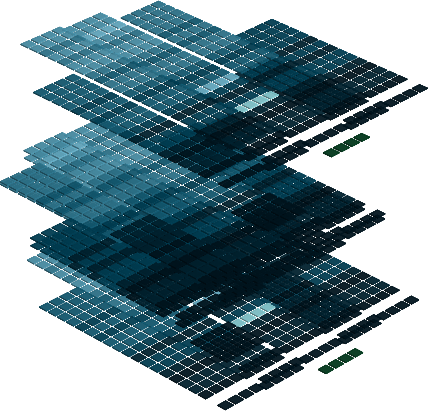
\includegraphics[width=1.5cm]{src/colorspace_colourflow/flows/colourflow_160-45.png}%           
  \end{adjustbox}                                                        
\caption*{

\begin{tikzpicture}                             
\definecolor{tempcolor}{HTML}{000000}           
\fill[tempcolor] (1 mm,0) rectangle ++(1mm,1mm);
\definecolor{tempcolor}{HTML}{001a26}           
\fill[tempcolor] (2 mm,0) rectangle ++(1mm,1mm);
\definecolor{tempcolor}{HTML}{002b3c}           
\fill[tempcolor] (3 mm,0) rectangle ++(1mm,1mm);
\definecolor{tempcolor}{HTML}{004d68}           
\fill[tempcolor] (4 mm,0) rectangle ++(1mm,1mm);
\definecolor{tempcolor}{HTML}{176f8d}           
\fill[tempcolor] (5 mm,0) rectangle ++(1mm,1mm);
\definecolor{tempcolor}{HTML}{3991af}           
\fill[tempcolor] (6 mm,0) rectangle ++(1mm,1mm);
\definecolor{tempcolor}{HTML}{5bb3d1}           
\fill[tempcolor] (7 mm,0) rectangle ++(1mm,1mm);
\definecolor{tempcolor}{HTML}{7dd5f3}           
\fill[tempcolor] (8 mm,0) rectangle ++(1mm,1mm);
\end{tikzpicture}                               
}
\end{figure}                                                               
\end{minipage}
\hspace{0.1cm}
\begin{minipage}[b]{0.15\linewidth}
\begin{figure}[H]                                                          
  \centering                                                             
  \begin{adjustbox}{width=1.5cm,center}                                   
  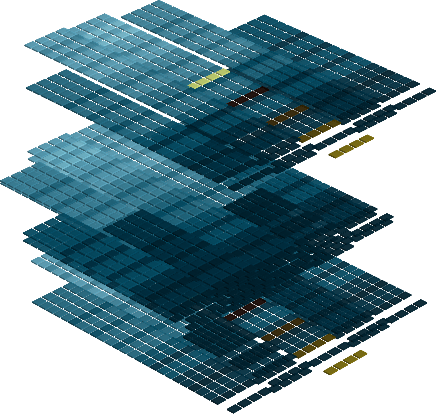
\includegraphics[width=1.5cm]{src/colorspace_colourflow/flows/colourflow_161-45.png}%           
  \end{adjustbox}                                                        
\caption*{

\begin{tikzpicture}                             
\definecolor{tempcolor}{HTML}{000000}           
\fill[tempcolor] (1 mm,0) rectangle ++(1mm,1mm);
\definecolor{tempcolor}{HTML}{002b3c}           
\fill[tempcolor] (2 mm,0) rectangle ++(1mm,1mm);
\definecolor{tempcolor}{HTML}{003c52}           
\fill[tempcolor] (3 mm,0) rectangle ++(1mm,1mm);
\definecolor{tempcolor}{HTML}{065e7c}           
\fill[tempcolor] (4 mm,0) rectangle ++(1mm,1mm);
\definecolor{tempcolor}{HTML}{28809e}           
\fill[tempcolor] (5 mm,0) rectangle ++(1mm,1mm);
\definecolor{tempcolor}{HTML}{4aa2c0}           
\fill[tempcolor] (6 mm,0) rectangle ++(1mm,1mm);
\definecolor{tempcolor}{HTML}{6cc4e2}           
\fill[tempcolor] (7 mm,0) rectangle ++(1mm,1mm);
\definecolor{tempcolor}{HTML}{8ee6ff}           
\fill[tempcolor] (8 mm,0) rectangle ++(1mm,1mm);
\end{tikzpicture}                               
}
\end{figure}                                                               
\end{minipage}
\hspace{0.1cm}
\begin{minipage}[b]{0.15\linewidth}
\begin{figure}[H]                                                          
  \centering                                                             
  \begin{adjustbox}{width=1.5cm,center}                                   
  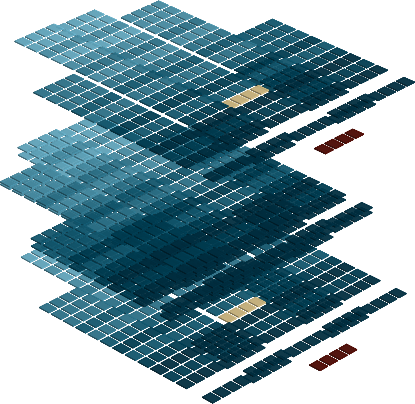
\includegraphics[width=1.5cm]{src/colorspace_colourflow/flows/colourflow_162-45.png}%           
  \end{adjustbox}                                                        
\caption*{

\begin{tikzpicture}                             
\definecolor{tempcolor}{HTML}{000000}           
\fill[tempcolor] (1 mm,0) rectangle ++(1mm,1mm);
\definecolor{tempcolor}{HTML}{003c52}           
\fill[tempcolor] (2 mm,0) rectangle ++(1mm,1mm);
\definecolor{tempcolor}{HTML}{004d68}           
\fill[tempcolor] (3 mm,0) rectangle ++(1mm,1mm);
\definecolor{tempcolor}{HTML}{176f8d}           
\fill[tempcolor] (4 mm,0) rectangle ++(1mm,1mm);
\definecolor{tempcolor}{HTML}{3991af}           
\fill[tempcolor] (5 mm,0) rectangle ++(1mm,1mm);
\definecolor{tempcolor}{HTML}{5bb3d1}           
\fill[tempcolor] (6 mm,0) rectangle ++(1mm,1mm);
\definecolor{tempcolor}{HTML}{7dd5f3}           
\fill[tempcolor] (7 mm,0) rectangle ++(1mm,1mm);
\definecolor{tempcolor}{HTML}{9ff7ff}           
\fill[tempcolor] (8 mm,0) rectangle ++(1mm,1mm);
\end{tikzpicture}                               
}
\end{figure}                                                               
\end{minipage}
\hspace{0.1cm}
\begin{minipage}[b]{0.15\linewidth}
\begin{figure}[H]                                                          
  \centering                                                             
  \begin{adjustbox}{width=1.5cm,center}                                   
  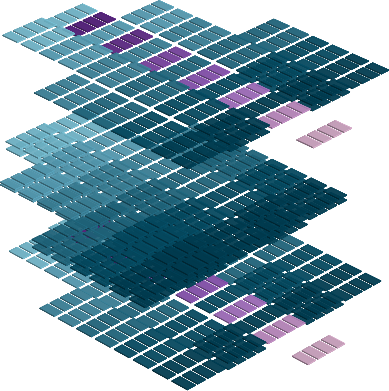
\includegraphics[width=1.5cm]{src/colorspace_colourflow/flows/colourflow_163-45.png}%           
  \end{adjustbox}                                                        
\caption*{

\begin{tikzpicture}                             
\definecolor{tempcolor}{HTML}{000000}           
\fill[tempcolor] (1 mm,0) rectangle ++(1mm,1mm);
\definecolor{tempcolor}{HTML}{004d68}           
\fill[tempcolor] (2 mm,0) rectangle ++(1mm,1mm);
\definecolor{tempcolor}{HTML}{065e7c}           
\fill[tempcolor] (3 mm,0) rectangle ++(1mm,1mm);
\definecolor{tempcolor}{HTML}{28809e}           
\fill[tempcolor] (4 mm,0) rectangle ++(1mm,1mm);
\definecolor{tempcolor}{HTML}{4aa2c0}           
\fill[tempcolor] (5 mm,0) rectangle ++(1mm,1mm);
\definecolor{tempcolor}{HTML}{6cc4e2}           
\fill[tempcolor] (6 mm,0) rectangle ++(1mm,1mm);
\definecolor{tempcolor}{HTML}{8ee6ff}           
\fill[tempcolor] (7 mm,0) rectangle ++(1mm,1mm);
\definecolor{tempcolor}{HTML}{b0ffff}           
\fill[tempcolor] (8 mm,0) rectangle ++(1mm,1mm);
\end{tikzpicture}                               
}
\end{figure}                                                               
\end{minipage}
\hspace{0.1cm}
\begin{minipage}[b]{0.15\linewidth}
\begin{figure}[H]                                                          
  \centering                                                             
  \begin{adjustbox}{width=1.5cm,center}                                   
  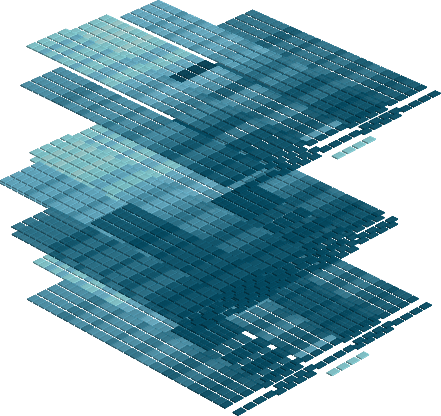
\includegraphics[width=1.5cm]{src/colorspace_colourflow/flows/colourflow_164-45.png}%           
  \end{adjustbox}                                                        
\caption*{

\begin{tikzpicture}                             
\definecolor{tempcolor}{HTML}{000000}           
\fill[tempcolor] (1 mm,0) rectangle ++(1mm,1mm);
\definecolor{tempcolor}{HTML}{065e7c}           
\fill[tempcolor] (2 mm,0) rectangle ++(1mm,1mm);
\definecolor{tempcolor}{HTML}{176f8d}           
\fill[tempcolor] (3 mm,0) rectangle ++(1mm,1mm);
\definecolor{tempcolor}{HTML}{3991af}           
\fill[tempcolor] (4 mm,0) rectangle ++(1mm,1mm);
\definecolor{tempcolor}{HTML}{5bb3d1}           
\fill[tempcolor] (5 mm,0) rectangle ++(1mm,1mm);
\definecolor{tempcolor}{HTML}{7dd5f3}           
\fill[tempcolor] (6 mm,0) rectangle ++(1mm,1mm);
\definecolor{tempcolor}{HTML}{9ff7ff}           
\fill[tempcolor] (7 mm,0) rectangle ++(1mm,1mm);
\definecolor{tempcolor}{HTML}{c1ffff}           
\fill[tempcolor] (8 mm,0) rectangle ++(1mm,1mm);
\end{tikzpicture}                               
}
\end{figure}                                                               
\end{minipage}
\hspace{0.1cm}
\begin{minipage}[b]{0.15\linewidth}
\begin{figure}[H]                                                          
  \centering                                                             
  \begin{adjustbox}{width=1.5cm,center}                                   
  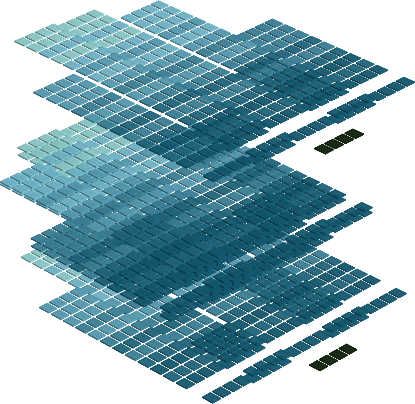
\includegraphics[width=1.5cm]{src/colorspace_colourflow/flows/colourflow_165-45.png}%           
  \end{adjustbox}                                                        
\caption*{

\begin{tikzpicture}                             
\definecolor{tempcolor}{HTML}{000000}           
\fill[tempcolor] (1 mm,0) rectangle ++(1mm,1mm);
\definecolor{tempcolor}{HTML}{176f8d}           
\fill[tempcolor] (2 mm,0) rectangle ++(1mm,1mm);
\definecolor{tempcolor}{HTML}{28809e}           
\fill[tempcolor] (3 mm,0) rectangle ++(1mm,1mm);
\definecolor{tempcolor}{HTML}{4aa2c0}           
\fill[tempcolor] (4 mm,0) rectangle ++(1mm,1mm);
\definecolor{tempcolor}{HTML}{6cc4e2}           
\fill[tempcolor] (5 mm,0) rectangle ++(1mm,1mm);
\definecolor{tempcolor}{HTML}{8ee6ff}           
\fill[tempcolor] (6 mm,0) rectangle ++(1mm,1mm);
\definecolor{tempcolor}{HTML}{b0ffff}           
\fill[tempcolor] (7 mm,0) rectangle ++(1mm,1mm);
\definecolor{tempcolor}{HTML}{01250a}           
\fill[tempcolor] (8 mm,0) rectangle ++(1mm,1mm);
\end{tikzpicture}                               
}
\end{figure}                                                               
\end{minipage}
\hspace{0.1cm}
\begin{minipage}[b]{0.15\linewidth}
\begin{figure}[H]                                                          
  \centering                                                             
  \begin{adjustbox}{width=1.5cm,center}                                   
  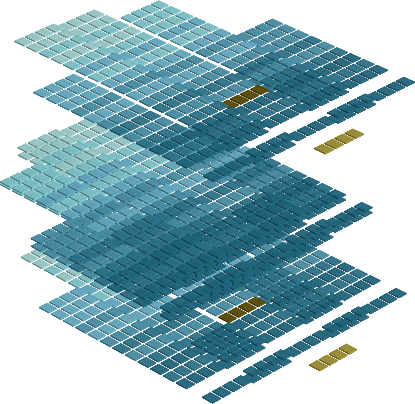
\includegraphics[width=1.5cm]{src/colorspace_colourflow/flows/colourflow_166-45.png}%           
  \end{adjustbox}                                                        
\caption*{

\begin{tikzpicture}                             
\definecolor{tempcolor}{HTML}{000000}           
\fill[tempcolor] (1 mm,0) rectangle ++(1mm,1mm);
\definecolor{tempcolor}{HTML}{28809e}           
\fill[tempcolor] (2 mm,0) rectangle ++(1mm,1mm);
\definecolor{tempcolor}{HTML}{3991af}           
\fill[tempcolor] (3 mm,0) rectangle ++(1mm,1mm);
\definecolor{tempcolor}{HTML}{5bb3d1}           
\fill[tempcolor] (4 mm,0) rectangle ++(1mm,1mm);
\definecolor{tempcolor}{HTML}{7dd5f3}           
\fill[tempcolor] (5 mm,0) rectangle ++(1mm,1mm);
\definecolor{tempcolor}{HTML}{9ff7ff}           
\fill[tempcolor] (6 mm,0) rectangle ++(1mm,1mm);
\definecolor{tempcolor}{HTML}{c1ffff}           
\fill[tempcolor] (7 mm,0) rectangle ++(1mm,1mm);
\definecolor{tempcolor}{HTML}{023610}           
\fill[tempcolor] (8 mm,0) rectangle ++(1mm,1mm);
\end{tikzpicture}                               
}
\end{figure}                                                               
\end{minipage}
\hspace{0.1cm}
\begin{minipage}[b]{0.15\linewidth}
\begin{figure}[H]                                                          
  \centering                                                             
  \begin{adjustbox}{width=1.5cm,center}                                   
  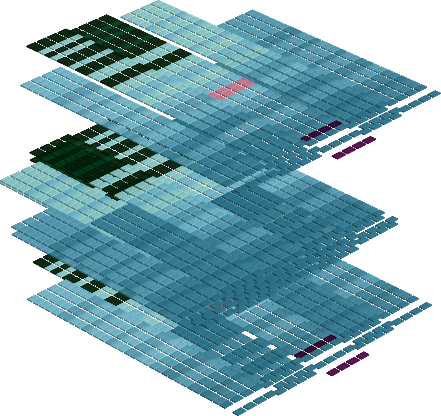
\includegraphics[width=1.5cm]{src/colorspace_colourflow/flows/colourflow_167-45.png}%           
  \end{adjustbox}                                                        
\caption*{

\begin{tikzpicture}                             
\definecolor{tempcolor}{HTML}{000000}           
\fill[tempcolor] (1 mm,0) rectangle ++(1mm,1mm);
\definecolor{tempcolor}{HTML}{3991af}           
\fill[tempcolor] (2 mm,0) rectangle ++(1mm,1mm);
\definecolor{tempcolor}{HTML}{4aa2c0}           
\fill[tempcolor] (3 mm,0) rectangle ++(1mm,1mm);
\definecolor{tempcolor}{HTML}{6cc4e2}           
\fill[tempcolor] (4 mm,0) rectangle ++(1mm,1mm);
\definecolor{tempcolor}{HTML}{8ee6ff}           
\fill[tempcolor] (5 mm,0) rectangle ++(1mm,1mm);
\definecolor{tempcolor}{HTML}{b0ffff}           
\fill[tempcolor] (6 mm,0) rectangle ++(1mm,1mm);
\definecolor{tempcolor}{HTML}{01250a}           
\fill[tempcolor] (7 mm,0) rectangle ++(1mm,1mm);
\definecolor{tempcolor}{HTML}{004622}           
\fill[tempcolor] (8 mm,0) rectangle ++(1mm,1mm);
\end{tikzpicture}                               
}
\end{figure}                                                               
\end{minipage}
\hspace{0.1cm}
\begin{minipage}[b]{0.15\linewidth}
\begin{figure}[H]                                                          
  \centering                                                             
  \begin{adjustbox}{width=1.5cm,center}                                   
  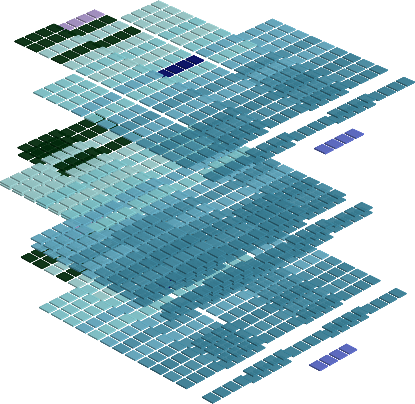
\includegraphics[width=1.5cm]{src/colorspace_colourflow/flows/colourflow_168-45.png}%           
  \end{adjustbox}                                                        
\caption*{

\begin{tikzpicture}                             
\definecolor{tempcolor}{HTML}{000000}           
\fill[tempcolor] (1 mm,0) rectangle ++(1mm,1mm);
\definecolor{tempcolor}{HTML}{4aa2c0}           
\fill[tempcolor] (2 mm,0) rectangle ++(1mm,1mm);
\definecolor{tempcolor}{HTML}{5bb3d1}           
\fill[tempcolor] (3 mm,0) rectangle ++(1mm,1mm);
\definecolor{tempcolor}{HTML}{7dd5f3}           
\fill[tempcolor] (4 mm,0) rectangle ++(1mm,1mm);
\definecolor{tempcolor}{HTML}{9ff7ff}           
\fill[tempcolor] (5 mm,0) rectangle ++(1mm,1mm);
\definecolor{tempcolor}{HTML}{c1ffff}           
\fill[tempcolor] (6 mm,0) rectangle ++(1mm,1mm);
\definecolor{tempcolor}{HTML}{023610}           
\fill[tempcolor] (7 mm,0) rectangle ++(1mm,1mm);
\definecolor{tempcolor}{HTML}{005738}           
\fill[tempcolor] (8 mm,0) rectangle ++(1mm,1mm);
\end{tikzpicture}                               
}
\end{figure}                                                               
\end{minipage}
\hspace{0.1cm}
\begin{minipage}[b]{0.15\linewidth}
\begin{figure}[H]                                                          
  \centering                                                             
  \begin{adjustbox}{width=1.5cm,center}                                   
  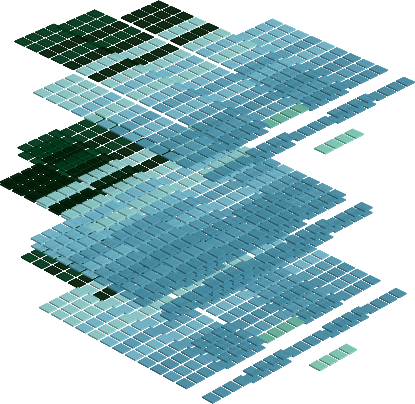
\includegraphics[width=1.5cm]{src/colorspace_colourflow/flows/colourflow_169-45.png}%           
  \end{adjustbox}                                                        
\caption*{

\begin{tikzpicture}                             
\definecolor{tempcolor}{HTML}{000000}           
\fill[tempcolor] (1 mm,0) rectangle ++(1mm,1mm);
\definecolor{tempcolor}{HTML}{5bb3d1}           
\fill[tempcolor] (2 mm,0) rectangle ++(1mm,1mm);
\definecolor{tempcolor}{HTML}{6cc4e2}           
\fill[tempcolor] (3 mm,0) rectangle ++(1mm,1mm);
\definecolor{tempcolor}{HTML}{8ee6ff}           
\fill[tempcolor] (4 mm,0) rectangle ++(1mm,1mm);
\definecolor{tempcolor}{HTML}{b0ffff}           
\fill[tempcolor] (5 mm,0) rectangle ++(1mm,1mm);
\definecolor{tempcolor}{HTML}{01250a}           
\fill[tempcolor] (6 mm,0) rectangle ++(1mm,1mm);
\definecolor{tempcolor}{HTML}{004622}           
\fill[tempcolor] (7 mm,0) rectangle ++(1mm,1mm);
\definecolor{tempcolor}{HTML}{05684d}           
\fill[tempcolor] (8 mm,0) rectangle ++(1mm,1mm);
\end{tikzpicture}                               
}
\end{figure}                                                               
\end{minipage}
\hspace{0.1cm}
\begin{minipage}[b]{0.15\linewidth}
\begin{figure}[H]                                                          
  \centering                                                             
  \begin{adjustbox}{width=1.5cm,center}                                   
  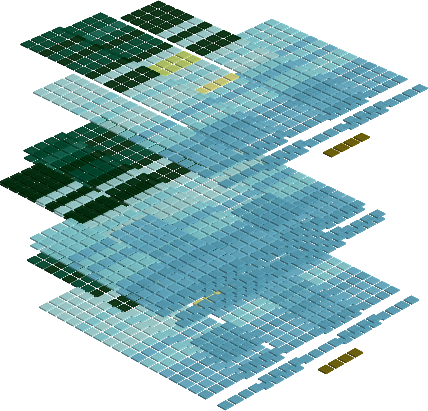
\includegraphics[width=1.5cm]{src/colorspace_colourflow/flows/colourflow_170-45.png}%           
  \end{adjustbox}                                                        
\caption*{

\begin{tikzpicture}                             
\definecolor{tempcolor}{HTML}{000000}           
\fill[tempcolor] (1 mm,0) rectangle ++(1mm,1mm);
\definecolor{tempcolor}{HTML}{6cc4e2}           
\fill[tempcolor] (2 mm,0) rectangle ++(1mm,1mm);
\definecolor{tempcolor}{HTML}{7dd5f3}           
\fill[tempcolor] (3 mm,0) rectangle ++(1mm,1mm);
\definecolor{tempcolor}{HTML}{9ff7ff}           
\fill[tempcolor] (4 mm,0) rectangle ++(1mm,1mm);
\definecolor{tempcolor}{HTML}{c1ffff}           
\fill[tempcolor] (5 mm,0) rectangle ++(1mm,1mm);
\definecolor{tempcolor}{HTML}{023610}           
\fill[tempcolor] (6 mm,0) rectangle ++(1mm,1mm);
\definecolor{tempcolor}{HTML}{005738}           
\fill[tempcolor] (7 mm,0) rectangle ++(1mm,1mm);
\definecolor{tempcolor}{HTML}{16795e}           
\fill[tempcolor] (8 mm,0) rectangle ++(1mm,1mm);
\end{tikzpicture}                               
}
\end{figure}                                                               
\end{minipage}
\hspace{0.1cm}
\begin{minipage}[b]{0.15\linewidth}
\begin{figure}[H]                                                          
  \centering                                                             
  \begin{adjustbox}{width=1.5cm,center}                                   
  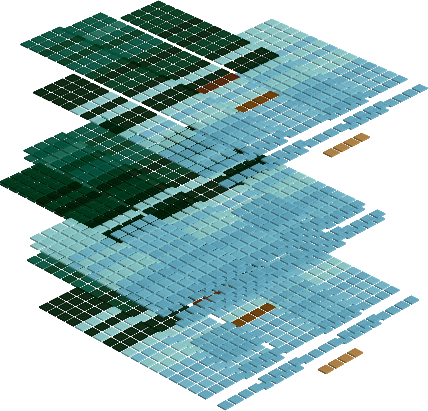
\includegraphics[width=1.5cm]{src/colorspace_colourflow/flows/colourflow_171-45.png}%           
  \end{adjustbox}                                                        
\caption*{

\begin{tikzpicture}                             
\definecolor{tempcolor}{HTML}{000000}           
\fill[tempcolor] (1 mm,0) rectangle ++(1mm,1mm);
\definecolor{tempcolor}{HTML}{7dd5f3}           
\fill[tempcolor] (2 mm,0) rectangle ++(1mm,1mm);
\definecolor{tempcolor}{HTML}{8ee6ff}           
\fill[tempcolor] (3 mm,0) rectangle ++(1mm,1mm);
\definecolor{tempcolor}{HTML}{b0ffff}           
\fill[tempcolor] (4 mm,0) rectangle ++(1mm,1mm);
\definecolor{tempcolor}{HTML}{01250a}           
\fill[tempcolor] (5 mm,0) rectangle ++(1mm,1mm);
\definecolor{tempcolor}{HTML}{004622}           
\fill[tempcolor] (6 mm,0) rectangle ++(1mm,1mm);
\definecolor{tempcolor}{HTML}{05684d}           
\fill[tempcolor] (7 mm,0) rectangle ++(1mm,1mm);
\definecolor{tempcolor}{HTML}{278a6f}           
\fill[tempcolor] (8 mm,0) rectangle ++(1mm,1mm);
\end{tikzpicture}                               
}
\end{figure}                                                               
\end{minipage}
\hspace{0.1cm}
\begin{minipage}[b]{0.15\linewidth}
\begin{figure}[H]                                                          
  \centering                                                             
  \begin{adjustbox}{width=1.5cm,center}                                   
  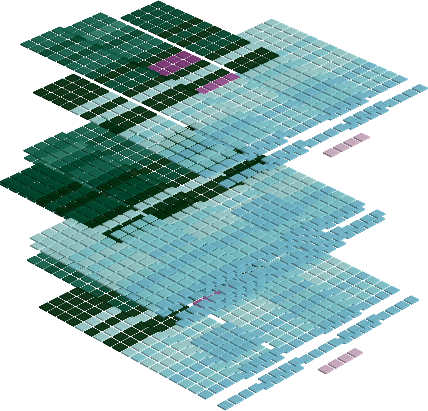
\includegraphics[width=1.5cm]{src/colorspace_colourflow/flows/colourflow_172-45.png}%           
  \end{adjustbox}                                                        
\caption*{

\begin{tikzpicture}                             
\definecolor{tempcolor}{HTML}{000000}           
\fill[tempcolor] (1 mm,0) rectangle ++(1mm,1mm);
\definecolor{tempcolor}{HTML}{8ee6ff}           
\fill[tempcolor] (2 mm,0) rectangle ++(1mm,1mm);
\definecolor{tempcolor}{HTML}{9ff7ff}           
\fill[tempcolor] (3 mm,0) rectangle ++(1mm,1mm);
\definecolor{tempcolor}{HTML}{c1ffff}           
\fill[tempcolor] (4 mm,0) rectangle ++(1mm,1mm);
\definecolor{tempcolor}{HTML}{023610}           
\fill[tempcolor] (5 mm,0) rectangle ++(1mm,1mm);
\definecolor{tempcolor}{HTML}{005738}           
\fill[tempcolor] (6 mm,0) rectangle ++(1mm,1mm);
\definecolor{tempcolor}{HTML}{16795e}           
\fill[tempcolor] (7 mm,0) rectangle ++(1mm,1mm);
\definecolor{tempcolor}{HTML}{389b80}           
\fill[tempcolor] (8 mm,0) rectangle ++(1mm,1mm);
\end{tikzpicture}                               
}
\end{figure}                                                               
\end{minipage}
\hspace{0.1cm}
\begin{minipage}[b]{0.15\linewidth}
\begin{figure}[H]                                                          
  \centering                                                             
  \begin{adjustbox}{width=1.5cm,center}                                   
  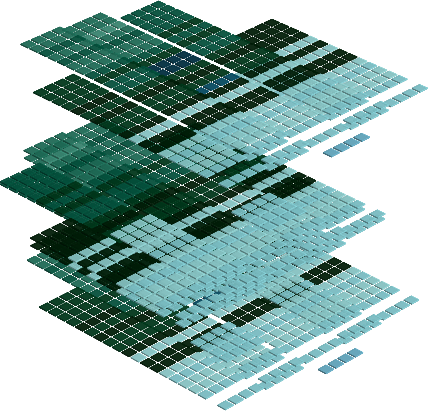
\includegraphics[width=1.5cm]{src/colorspace_colourflow/flows/colourflow_173-45.png}%           
  \end{adjustbox}                                                        
\caption*{

\begin{tikzpicture}                             
\definecolor{tempcolor}{HTML}{000000}           
\fill[tempcolor] (1 mm,0) rectangle ++(1mm,1mm);
\definecolor{tempcolor}{HTML}{9ff7ff}           
\fill[tempcolor] (2 mm,0) rectangle ++(1mm,1mm);
\definecolor{tempcolor}{HTML}{b0ffff}           
\fill[tempcolor] (3 mm,0) rectangle ++(1mm,1mm);
\definecolor{tempcolor}{HTML}{01250a}           
\fill[tempcolor] (4 mm,0) rectangle ++(1mm,1mm);
\definecolor{tempcolor}{HTML}{004622}           
\fill[tempcolor] (5 mm,0) rectangle ++(1mm,1mm);
\definecolor{tempcolor}{HTML}{05684d}           
\fill[tempcolor] (6 mm,0) rectangle ++(1mm,1mm);
\definecolor{tempcolor}{HTML}{278a6f}           
\fill[tempcolor] (7 mm,0) rectangle ++(1mm,1mm);
\definecolor{tempcolor}{HTML}{49ac91}           
\fill[tempcolor] (8 mm,0) rectangle ++(1mm,1mm);
\end{tikzpicture}                               
}
\end{figure}                                                               
\end{minipage}
\hspace{0.1cm}
\begin{minipage}[b]{0.15\linewidth}
\begin{figure}[H]                                                          
  \centering                                                             
  \begin{adjustbox}{width=1.5cm,center}                                   
  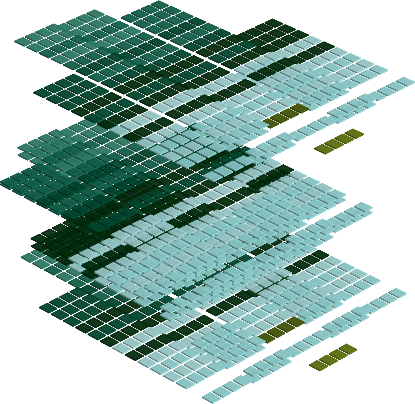
\includegraphics[width=1.5cm]{src/colorspace_colourflow/flows/colourflow_174-45.png}%           
  \end{adjustbox}                                                        
\caption*{

\begin{tikzpicture}                             
\definecolor{tempcolor}{HTML}{000000}           
\fill[tempcolor] (1 mm,0) rectangle ++(1mm,1mm);
\definecolor{tempcolor}{HTML}{b0ffff}           
\fill[tempcolor] (2 mm,0) rectangle ++(1mm,1mm);
\definecolor{tempcolor}{HTML}{c1ffff}           
\fill[tempcolor] (3 mm,0) rectangle ++(1mm,1mm);
\definecolor{tempcolor}{HTML}{023610}           
\fill[tempcolor] (4 mm,0) rectangle ++(1mm,1mm);
\definecolor{tempcolor}{HTML}{005738}           
\fill[tempcolor] (5 mm,0) rectangle ++(1mm,1mm);
\definecolor{tempcolor}{HTML}{16795e}           
\fill[tempcolor] (6 mm,0) rectangle ++(1mm,1mm);
\definecolor{tempcolor}{HTML}{389b80}           
\fill[tempcolor] (7 mm,0) rectangle ++(1mm,1mm);
\definecolor{tempcolor}{HTML}{5abda2}           
\fill[tempcolor] (8 mm,0) rectangle ++(1mm,1mm);
\end{tikzpicture}                               
}
\end{figure}                                                               
\end{minipage}
\hspace{0.1cm}
\begin{minipage}[b]{0.15\linewidth}
\begin{figure}[H]                                                          
  \centering                                                             
  \begin{adjustbox}{width=1.5cm,center}                                   
  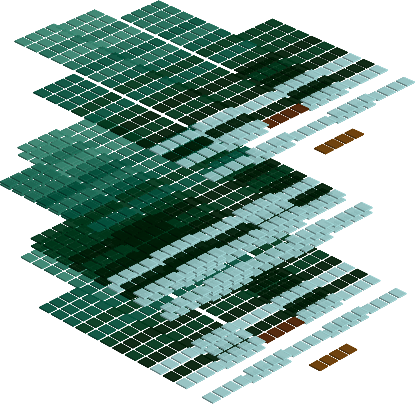
\includegraphics[width=1.5cm]{src/colorspace_colourflow/flows/colourflow_175-45.png}%           
  \end{adjustbox}                                                        
\caption*{

\begin{tikzpicture}                             
\definecolor{tempcolor}{HTML}{000000}           
\fill[tempcolor] (1 mm,0) rectangle ++(1mm,1mm);
\definecolor{tempcolor}{HTML}{c1ffff}           
\fill[tempcolor] (2 mm,0) rectangle ++(1mm,1mm);
\definecolor{tempcolor}{HTML}{01250a}           
\fill[tempcolor] (3 mm,0) rectangle ++(1mm,1mm);
\definecolor{tempcolor}{HTML}{004622}           
\fill[tempcolor] (4 mm,0) rectangle ++(1mm,1mm);
\definecolor{tempcolor}{HTML}{05684d}           
\fill[tempcolor] (5 mm,0) rectangle ++(1mm,1mm);
\definecolor{tempcolor}{HTML}{278a6f}           
\fill[tempcolor] (6 mm,0) rectangle ++(1mm,1mm);
\definecolor{tempcolor}{HTML}{49ac91}           
\fill[tempcolor] (7 mm,0) rectangle ++(1mm,1mm);
\definecolor{tempcolor}{HTML}{6bceb3}           
\fill[tempcolor] (8 mm,0) rectangle ++(1mm,1mm);
\end{tikzpicture}                               
}
\end{figure}                                                               
\end{minipage}
\hspace{0.1cm}
\begin{minipage}[b]{0.15\linewidth}
\begin{figure}[H]                                                          
  \centering                                                             
  \begin{adjustbox}{width=1.5cm,center}                                   
  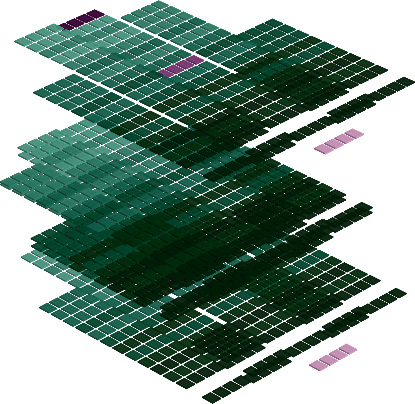
\includegraphics[width=1.5cm]{src/colorspace_colourflow/flows/colourflow_176-45.png}%           
  \end{adjustbox}                                                        
\caption*{

\begin{tikzpicture}                             
\definecolor{tempcolor}{HTML}{000000}           
\fill[tempcolor] (1 mm,0) rectangle ++(1mm,1mm);
\definecolor{tempcolor}{HTML}{01250a}           
\fill[tempcolor] (2 mm,0) rectangle ++(1mm,1mm);
\definecolor{tempcolor}{HTML}{023610}           
\fill[tempcolor] (3 mm,0) rectangle ++(1mm,1mm);
\definecolor{tempcolor}{HTML}{005738}           
\fill[tempcolor] (4 mm,0) rectangle ++(1mm,1mm);
\definecolor{tempcolor}{HTML}{16795e}           
\fill[tempcolor] (5 mm,0) rectangle ++(1mm,1mm);
\definecolor{tempcolor}{HTML}{389b80}           
\fill[tempcolor] (6 mm,0) rectangle ++(1mm,1mm);
\definecolor{tempcolor}{HTML}{5abda2}           
\fill[tempcolor] (7 mm,0) rectangle ++(1mm,1mm);
\definecolor{tempcolor}{HTML}{7cdfc4}           
\fill[tempcolor] (8 mm,0) rectangle ++(1mm,1mm);
\end{tikzpicture}                               
}
\end{figure}                                                               
\end{minipage}
\hspace{0.1cm}
\begin{minipage}[b]{0.15\linewidth}
\begin{figure}[H]                                                          
  \centering                                                             
  \begin{adjustbox}{width=1.5cm,center}                                   
  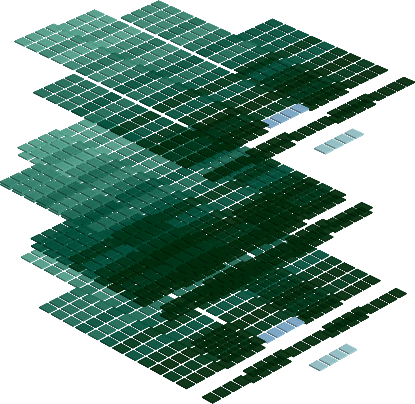
\includegraphics[width=1.5cm]{src/colorspace_colourflow/flows/colourflow_177-45.png}%           
  \end{adjustbox}                                                        
\caption*{

\begin{tikzpicture}                             
\definecolor{tempcolor}{HTML}{000000}           
\fill[tempcolor] (1 mm,0) rectangle ++(1mm,1mm);
\definecolor{tempcolor}{HTML}{023610}           
\fill[tempcolor] (2 mm,0) rectangle ++(1mm,1mm);
\definecolor{tempcolor}{HTML}{004622}           
\fill[tempcolor] (3 mm,0) rectangle ++(1mm,1mm);
\definecolor{tempcolor}{HTML}{05684d}           
\fill[tempcolor] (4 mm,0) rectangle ++(1mm,1mm);
\definecolor{tempcolor}{HTML}{278a6f}           
\fill[tempcolor] (5 mm,0) rectangle ++(1mm,1mm);
\definecolor{tempcolor}{HTML}{49ac91}           
\fill[tempcolor] (6 mm,0) rectangle ++(1mm,1mm);
\definecolor{tempcolor}{HTML}{6bceb3}           
\fill[tempcolor] (7 mm,0) rectangle ++(1mm,1mm);
\definecolor{tempcolor}{HTML}{8df0d5}           
\fill[tempcolor] (8 mm,0) rectangle ++(1mm,1mm);
\end{tikzpicture}                               
}
\end{figure}                                                               
\end{minipage}
\hspace{0.1cm}
\begin{minipage}[b]{0.15\linewidth}
\begin{figure}[H]                                                          
  \centering                                                             
  \begin{adjustbox}{width=1.5cm,center}                                   
  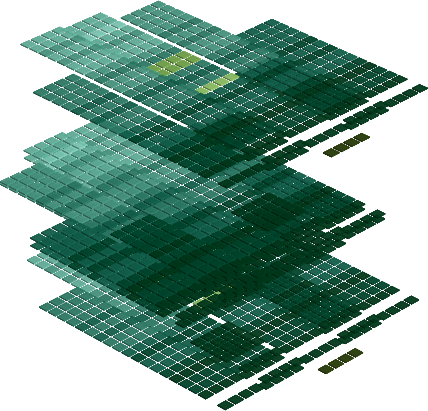
\includegraphics[width=1.5cm]{src/colorspace_colourflow/flows/colourflow_178-45.png}%           
  \end{adjustbox}                                                        
\caption*{

\begin{tikzpicture}                             
\definecolor{tempcolor}{HTML}{000000}           
\fill[tempcolor] (1 mm,0) rectangle ++(1mm,1mm);
\definecolor{tempcolor}{HTML}{004622}           
\fill[tempcolor] (2 mm,0) rectangle ++(1mm,1mm);
\definecolor{tempcolor}{HTML}{005738}           
\fill[tempcolor] (3 mm,0) rectangle ++(1mm,1mm);
\definecolor{tempcolor}{HTML}{16795e}           
\fill[tempcolor] (4 mm,0) rectangle ++(1mm,1mm);
\definecolor{tempcolor}{HTML}{389b80}           
\fill[tempcolor] (5 mm,0) rectangle ++(1mm,1mm);
\definecolor{tempcolor}{HTML}{5abda2}           
\fill[tempcolor] (6 mm,0) rectangle ++(1mm,1mm);
\definecolor{tempcolor}{HTML}{7cdfc4}           
\fill[tempcolor] (7 mm,0) rectangle ++(1mm,1mm);
\definecolor{tempcolor}{HTML}{9effe5}           
\fill[tempcolor] (8 mm,0) rectangle ++(1mm,1mm);
\end{tikzpicture}                               
}
\end{figure}                                                               
\end{minipage}
\hspace{0.1cm}
\begin{minipage}[b]{0.15\linewidth}
\begin{figure}[H]                                                          
  \centering                                                             
  \begin{adjustbox}{width=1.5cm,center}                                   
  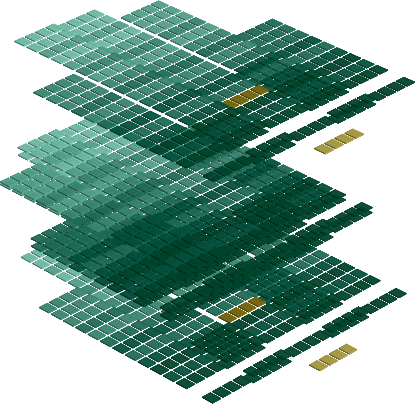
\includegraphics[width=1.5cm]{src/colorspace_colourflow/flows/colourflow_179-45.png}%           
  \end{adjustbox}                                                        
\caption*{

\begin{tikzpicture}                             
\definecolor{tempcolor}{HTML}{000000}           
\fill[tempcolor] (1 mm,0) rectangle ++(1mm,1mm);
\definecolor{tempcolor}{HTML}{005738}           
\fill[tempcolor] (2 mm,0) rectangle ++(1mm,1mm);
\definecolor{tempcolor}{HTML}{05684d}           
\fill[tempcolor] (3 mm,0) rectangle ++(1mm,1mm);
\definecolor{tempcolor}{HTML}{278a6f}           
\fill[tempcolor] (4 mm,0) rectangle ++(1mm,1mm);
\definecolor{tempcolor}{HTML}{49ac91}           
\fill[tempcolor] (5 mm,0) rectangle ++(1mm,1mm);
\definecolor{tempcolor}{HTML}{6bceb3}           
\fill[tempcolor] (6 mm,0) rectangle ++(1mm,1mm);
\definecolor{tempcolor}{HTML}{8df0d5}           
\fill[tempcolor] (7 mm,0) rectangle ++(1mm,1mm);
\definecolor{tempcolor}{HTML}{affff1}           
\fill[tempcolor] (8 mm,0) rectangle ++(1mm,1mm);
\end{tikzpicture}                               
}
\end{figure}                                                               
\end{minipage}
\hspace{0.1cm}
\begin{minipage}[b]{0.15\linewidth}
\begin{figure}[H]                                                          
  \centering                                                             
  \begin{adjustbox}{width=1.5cm,center}                                   
  \includegraphics[width=1.5cm]{src/colorspace_colourflow/flows/colourflow_180-45.png}%           
  \end{adjustbox}                                                        
\caption*{
\begin{tikzpicture}                             
\definecolor{tempcolor}{HTML}{000000}           
\fill[tempcolor] (1 mm,0) rectangle ++(1mm,1mm);
\definecolor{tempcolor}{HTML}{05684d}           
\fill[tempcolor] (2 mm,0) rectangle ++(1mm,1mm);
\definecolor{tempcolor}{HTML}{16795e}           
\fill[tempcolor] (3 mm,0) rectangle ++(1mm,1mm);
\definecolor{tempcolor}{HTML}{389b80}           
\fill[tempcolor] (4 mm,0) rectangle ++(1mm,1mm);
\definecolor{tempcolor}{HTML}{5abda2}           
\fill[tempcolor] (5 mm,0) rectangle ++(1mm,1mm);
\definecolor{tempcolor}{HTML}{7cdfc4}           
\fill[tempcolor] (6 mm,0) rectangle ++(1mm,1mm);
\definecolor{tempcolor}{HTML}{9effe5}           
\fill[tempcolor] (7 mm,0) rectangle ++(1mm,1mm);
\definecolor{tempcolor}{HTML}{c0fffd}           
\fill[tempcolor] (8 mm,0) rectangle ++(1mm,1mm);
\end{tikzpicture}                               
}
\end{figure}                                                               
\end{minipage}
\hspace{0.1cm}
\begin{minipage}[b]{0.15\linewidth}
\begin{figure}[H]                                                          
  \centering                                                             
  \begin{adjustbox}{width=1.5cm,center}                                   
  \includegraphics[width=1.5cm]{src/colorspace_colourflow/flows/colourflow_181-45.png}%           
  \end{adjustbox}                                                        
\caption*{
\begin{tikzpicture}                             
\definecolor{tempcolor}{HTML}{000000}           
\fill[tempcolor] (1 mm,0) rectangle ++(1mm,1mm);
\definecolor{tempcolor}{HTML}{16795e}           
\fill[tempcolor] (2 mm,0) rectangle ++(1mm,1mm);
\definecolor{tempcolor}{HTML}{278a6f}           
\fill[tempcolor] (3 mm,0) rectangle ++(1mm,1mm);
\definecolor{tempcolor}{HTML}{49ac91}           
\fill[tempcolor] (4 mm,0) rectangle ++(1mm,1mm);
\definecolor{tempcolor}{HTML}{6bceb3}           
\fill[tempcolor] (5 mm,0) rectangle ++(1mm,1mm);
\definecolor{tempcolor}{HTML}{8df0d5}           
\fill[tempcolor] (6 mm,0) rectangle ++(1mm,1mm);
\definecolor{tempcolor}{HTML}{affff1}           
\fill[tempcolor] (7 mm,0) rectangle ++(1mm,1mm);
\definecolor{tempcolor}{HTML}{04260d}           
\fill[tempcolor] (8 mm,0) rectangle ++(1mm,1mm);
\end{tikzpicture}                               
}
\end{figure}                                                               
\end{minipage}
\hspace{0.1cm}
\begin{minipage}[b]{0.15\linewidth}
\begin{figure}[H]                                                          
  \centering                                                             
  \begin{adjustbox}{width=1.5cm,center}                                   
  \includegraphics[width=1.5cm]{src/colorspace_colourflow/flows/colourflow_182-45.png}%           
  \end{adjustbox}                                                        
\caption*{
\begin{tikzpicture}                             
\definecolor{tempcolor}{HTML}{000000}           
\fill[tempcolor] (1 mm,0) rectangle ++(1mm,1mm);
\definecolor{tempcolor}{HTML}{278a6f}           
\fill[tempcolor] (2 mm,0) rectangle ++(1mm,1mm);
\definecolor{tempcolor}{HTML}{389b80}           
\fill[tempcolor] (3 mm,0) rectangle ++(1mm,1mm);
\definecolor{tempcolor}{HTML}{5abda2}           
\fill[tempcolor] (4 mm,0) rectangle ++(1mm,1mm);
\definecolor{tempcolor}{HTML}{7cdfc4}           
\fill[tempcolor] (5 mm,0) rectangle ++(1mm,1mm);
\definecolor{tempcolor}{HTML}{9effe5}           
\fill[tempcolor] (6 mm,0) rectangle ++(1mm,1mm);
\definecolor{tempcolor}{HTML}{c0fffd}           
\fill[tempcolor] (7 mm,0) rectangle ++(1mm,1mm);
\definecolor{tempcolor}{HTML}{043811}           
\fill[tempcolor] (8 mm,0) rectangle ++(1mm,1mm);
\end{tikzpicture}                               
}
\end{figure}                                                               
\end{minipage}
\hspace{0.1cm}
\begin{minipage}[b]{0.15\linewidth}
\begin{figure}[H]                                                          
  \centering                                                             
  \begin{adjustbox}{width=1.5cm,center}                                   
  \includegraphics[width=1.5cm]{src/colorspace_colourflow/flows/colourflow_183-45.png}%           
  \end{adjustbox}                                                        
\caption*{
\begin{tikzpicture}                             
\definecolor{tempcolor}{HTML}{000000}           
\fill[tempcolor] (1 mm,0) rectangle ++(1mm,1mm);
\definecolor{tempcolor}{HTML}{389b80}           
\fill[tempcolor] (2 mm,0) rectangle ++(1mm,1mm);
\definecolor{tempcolor}{HTML}{49ac91}           
\fill[tempcolor] (3 mm,0) rectangle ++(1mm,1mm);
\definecolor{tempcolor}{HTML}{6bceb3}           
\fill[tempcolor] (4 mm,0) rectangle ++(1mm,1mm);
\definecolor{tempcolor}{HTML}{8df0d5}           
\fill[tempcolor] (5 mm,0) rectangle ++(1mm,1mm);
\definecolor{tempcolor}{HTML}{affff1}           
\fill[tempcolor] (6 mm,0) rectangle ++(1mm,1mm);
\definecolor{tempcolor}{HTML}{04260d}           
\fill[tempcolor] (7 mm,0) rectangle ++(1mm,1mm);
\definecolor{tempcolor}{HTML}{054713}           
\fill[tempcolor] (8 mm,0) rectangle ++(1mm,1mm);
\end{tikzpicture}                               
}
\end{figure}                                                               
\end{minipage}
\hspace{0.1cm}
\begin{minipage}[b]{0.15\linewidth}
\begin{figure}[H]                                                          
  \centering                                                             
  \begin{adjustbox}{width=1.5cm,center}                                   
  \includegraphics[width=1.5cm]{src/colorspace_colourflow/flows/colourflow_184-45.png}%           
  \end{adjustbox}                                                        
\caption*{
\begin{tikzpicture}                             
\definecolor{tempcolor}{HTML}{000000}           
\fill[tempcolor] (1 mm,0) rectangle ++(1mm,1mm);
\definecolor{tempcolor}{HTML}{49ac91}           
\fill[tempcolor] (2 mm,0) rectangle ++(1mm,1mm);
\definecolor{tempcolor}{HTML}{5abda2}           
\fill[tempcolor] (3 mm,0) rectangle ++(1mm,1mm);
\definecolor{tempcolor}{HTML}{7cdfc4}           
\fill[tempcolor] (4 mm,0) rectangle ++(1mm,1mm);
\definecolor{tempcolor}{HTML}{9effe5}           
\fill[tempcolor] (5 mm,0) rectangle ++(1mm,1mm);
\definecolor{tempcolor}{HTML}{c0fffd}           
\fill[tempcolor] (6 mm,0) rectangle ++(1mm,1mm);
\definecolor{tempcolor}{HTML}{043811}           
\fill[tempcolor] (7 mm,0) rectangle ++(1mm,1mm);
\definecolor{tempcolor}{HTML}{005a1b}           
\fill[tempcolor] (8 mm,0) rectangle ++(1mm,1mm);
\end{tikzpicture}                               
}
\end{figure}                                                               
\end{minipage}
\hspace{0.1cm}
\begin{minipage}[b]{0.15\linewidth}
\begin{figure}[H]                                                          
  \centering                                                             
  \begin{adjustbox}{width=1.5cm,center}                                   
  \includegraphics[width=1.5cm]{src/colorspace_colourflow/flows/colourflow_185-45.png}%           
  \end{adjustbox}                                                        
\caption*{
\begin{tikzpicture}                             
\definecolor{tempcolor}{HTML}{000000}           
\fill[tempcolor] (1 mm,0) rectangle ++(1mm,1mm);
\definecolor{tempcolor}{HTML}{5abda2}           
\fill[tempcolor] (2 mm,0) rectangle ++(1mm,1mm);
\definecolor{tempcolor}{HTML}{6bceb3}           
\fill[tempcolor] (3 mm,0) rectangle ++(1mm,1mm);
\definecolor{tempcolor}{HTML}{8df0d5}           
\fill[tempcolor] (4 mm,0) rectangle ++(1mm,1mm);
\definecolor{tempcolor}{HTML}{affff1}           
\fill[tempcolor] (5 mm,0) rectangle ++(1mm,1mm);
\definecolor{tempcolor}{HTML}{04260d}           
\fill[tempcolor] (6 mm,0) rectangle ++(1mm,1mm);
\definecolor{tempcolor}{HTML}{054713}           
\fill[tempcolor] (7 mm,0) rectangle ++(1mm,1mm);
\definecolor{tempcolor}{HTML}{106b1b}           
\fill[tempcolor] (8 mm,0) rectangle ++(1mm,1mm);
\end{tikzpicture}                               
}
\end{figure}                                                               
\end{minipage}
\hspace{0.1cm}
\begin{minipage}[b]{0.15\linewidth}
\begin{figure}[H]                                                          
  \centering                                                             
  \begin{adjustbox}{width=1.5cm,center}                                   
  \includegraphics[width=1.5cm]{src/colorspace_colourflow/flows/colourflow_186-45.png}%           
  \end{adjustbox}                                                        
\caption*{
\begin{tikzpicture}                             
\definecolor{tempcolor}{HTML}{000000}           
\fill[tempcolor] (1 mm,0) rectangle ++(1mm,1mm);
\definecolor{tempcolor}{HTML}{6bceb3}           
\fill[tempcolor] (2 mm,0) rectangle ++(1mm,1mm);
\definecolor{tempcolor}{HTML}{7cdfc4}           
\fill[tempcolor] (3 mm,0) rectangle ++(1mm,1mm);
\definecolor{tempcolor}{HTML}{9effe5}           
\fill[tempcolor] (4 mm,0) rectangle ++(1mm,1mm);
\definecolor{tempcolor}{HTML}{c0fffd}           
\fill[tempcolor] (5 mm,0) rectangle ++(1mm,1mm);
\definecolor{tempcolor}{HTML}{043811}           
\fill[tempcolor] (6 mm,0) rectangle ++(1mm,1mm);
\definecolor{tempcolor}{HTML}{005a1b}           
\fill[tempcolor] (7 mm,0) rectangle ++(1mm,1mm);
\definecolor{tempcolor}{HTML}{217c2c}           
\fill[tempcolor] (8 mm,0) rectangle ++(1mm,1mm);
\end{tikzpicture}                               
}
\end{figure}                                                               
\end{minipage}
\hspace{0.1cm}
\begin{minipage}[b]{0.15\linewidth}
\begin{figure}[H]                                                          
  \centering                                                             
  \begin{adjustbox}{width=1.5cm,center}                                   
  \includegraphics[width=1.5cm]{src/colorspace_colourflow/flows/colourflow_187-45.png}%           
  \end{adjustbox}                                                        
\caption*{
\begin{tikzpicture}                             
\definecolor{tempcolor}{HTML}{000000}           
\fill[tempcolor] (1 mm,0) rectangle ++(1mm,1mm);
\definecolor{tempcolor}{HTML}{7cdfc4}           
\fill[tempcolor] (2 mm,0) rectangle ++(1mm,1mm);
\definecolor{tempcolor}{HTML}{8df0d5}           
\fill[tempcolor] (3 mm,0) rectangle ++(1mm,1mm);
\definecolor{tempcolor}{HTML}{affff1}           
\fill[tempcolor] (4 mm,0) rectangle ++(1mm,1mm);
\definecolor{tempcolor}{HTML}{04260d}           
\fill[tempcolor] (5 mm,0) rectangle ++(1mm,1mm);
\definecolor{tempcolor}{HTML}{054713}           
\fill[tempcolor] (6 mm,0) rectangle ++(1mm,1mm);
\definecolor{tempcolor}{HTML}{106b1b}           
\fill[tempcolor] (7 mm,0) rectangle ++(1mm,1mm);
\definecolor{tempcolor}{HTML}{328d3d}           
\fill[tempcolor] (8 mm,0) rectangle ++(1mm,1mm);
\end{tikzpicture}                               
}
\end{figure}                                                               
\end{minipage}
\hspace{0.1cm}
\begin{minipage}[b]{0.15\linewidth}
\begin{figure}[H]                                                          
  \centering                                                             
  \begin{adjustbox}{width=1.5cm,center}                                   
  \includegraphics[width=1.5cm]{src/colorspace_colourflow/flows/colourflow_188-45.png}%           
  \end{adjustbox}                                                        
\caption*{
\begin{tikzpicture}                             
\definecolor{tempcolor}{HTML}{000000}           
\fill[tempcolor] (1 mm,0) rectangle ++(1mm,1mm);
\definecolor{tempcolor}{HTML}{8df0d5}           
\fill[tempcolor] (2 mm,0) rectangle ++(1mm,1mm);
\definecolor{tempcolor}{HTML}{9effe5}           
\fill[tempcolor] (3 mm,0) rectangle ++(1mm,1mm);
\definecolor{tempcolor}{HTML}{c0fffd}           
\fill[tempcolor] (4 mm,0) rectangle ++(1mm,1mm);
\definecolor{tempcolor}{HTML}{043811}           
\fill[tempcolor] (5 mm,0) rectangle ++(1mm,1mm);
\definecolor{tempcolor}{HTML}{005a1b}           
\fill[tempcolor] (6 mm,0) rectangle ++(1mm,1mm);
\definecolor{tempcolor}{HTML}{217c2c}           
\fill[tempcolor] (7 mm,0) rectangle ++(1mm,1mm);
\definecolor{tempcolor}{HTML}{439e4e}           
\fill[tempcolor] (8 mm,0) rectangle ++(1mm,1mm);
\end{tikzpicture}                               
}
\end{figure}                                                               
\end{minipage}
\hspace{0.1cm}
\begin{minipage}[b]{0.15\linewidth}
\begin{figure}[H]                                                          
  \centering                                                             
  \begin{adjustbox}{width=1.5cm,center}                                   
  \includegraphics[width=1.5cm]{src/colorspace_colourflow/flows/colourflow_189-45.png}%           
  \end{adjustbox}                                                        
\caption*{
\begin{tikzpicture}                             
\definecolor{tempcolor}{HTML}{000000}           
\fill[tempcolor] (1 mm,0) rectangle ++(1mm,1mm);
\definecolor{tempcolor}{HTML}{9effe5}           
\fill[tempcolor] (2 mm,0) rectangle ++(1mm,1mm);
\definecolor{tempcolor}{HTML}{affff1}           
\fill[tempcolor] (3 mm,0) rectangle ++(1mm,1mm);
\definecolor{tempcolor}{HTML}{04260d}           
\fill[tempcolor] (4 mm,0) rectangle ++(1mm,1mm);
\definecolor{tempcolor}{HTML}{054713}           
\fill[tempcolor] (5 mm,0) rectangle ++(1mm,1mm);
\definecolor{tempcolor}{HTML}{106b1b}           
\fill[tempcolor] (6 mm,0) rectangle ++(1mm,1mm);
\definecolor{tempcolor}{HTML}{328d3d}           
\fill[tempcolor] (7 mm,0) rectangle ++(1mm,1mm);
\definecolor{tempcolor}{HTML}{54af5f}           
\fill[tempcolor] (8 mm,0) rectangle ++(1mm,1mm);
\end{tikzpicture}                               
}
\end{figure}                                                               
\end{minipage}
\hspace{0.1cm}
\begin{minipage}[b]{0.15\linewidth}
\begin{figure}[H]                                                          
  \centering                                                             
  \begin{adjustbox}{width=1.5cm,center}                                   
  \includegraphics[width=1.5cm]{src/colorspace_colourflow/flows/colourflow_190-45.png}%           
  \end{adjustbox}                                                        
\caption*{
\begin{tikzpicture}                             
\definecolor{tempcolor}{HTML}{000000}           
\fill[tempcolor] (1 mm,0) rectangle ++(1mm,1mm);
\definecolor{tempcolor}{HTML}{affff1}           
\fill[tempcolor] (2 mm,0) rectangle ++(1mm,1mm);
\definecolor{tempcolor}{HTML}{c0fffd}           
\fill[tempcolor] (3 mm,0) rectangle ++(1mm,1mm);
\definecolor{tempcolor}{HTML}{043811}           
\fill[tempcolor] (4 mm,0) rectangle ++(1mm,1mm);
\definecolor{tempcolor}{HTML}{005a1b}           
\fill[tempcolor] (5 mm,0) rectangle ++(1mm,1mm);
\definecolor{tempcolor}{HTML}{217c2c}           
\fill[tempcolor] (6 mm,0) rectangle ++(1mm,1mm);
\definecolor{tempcolor}{HTML}{439e4e}           
\fill[tempcolor] (7 mm,0) rectangle ++(1mm,1mm);
\definecolor{tempcolor}{HTML}{65c070}           
\fill[tempcolor] (8 mm,0) rectangle ++(1mm,1mm);
\end{tikzpicture}                               
}
\end{figure}                                                               
\end{minipage}
\hspace{0.1cm}
\begin{minipage}[b]{0.15\linewidth}
\begin{figure}[H]                                                          
  \centering                                                             
  \begin{adjustbox}{width=1.5cm,center}                                   
  \includegraphics[width=1.5cm]{src/colorspace_colourflow/flows/colourflow_191-45.png}%           
  \end{adjustbox}                                                        
\caption*{
\begin{tikzpicture}                             
\definecolor{tempcolor}{HTML}{000000}           
\fill[tempcolor] (1 mm,0) rectangle ++(1mm,1mm);
\definecolor{tempcolor}{HTML}{c0fffd}           
\fill[tempcolor] (2 mm,0) rectangle ++(1mm,1mm);
\definecolor{tempcolor}{HTML}{04260d}           
\fill[tempcolor] (3 mm,0) rectangle ++(1mm,1mm);
\definecolor{tempcolor}{HTML}{054713}           
\fill[tempcolor] (4 mm,0) rectangle ++(1mm,1mm);
\definecolor{tempcolor}{HTML}{106b1b}           
\fill[tempcolor] (5 mm,0) rectangle ++(1mm,1mm);
\definecolor{tempcolor}{HTML}{328d3d}           
\fill[tempcolor] (6 mm,0) rectangle ++(1mm,1mm);
\definecolor{tempcolor}{HTML}{54af5f}           
\fill[tempcolor] (7 mm,0) rectangle ++(1mm,1mm);
\definecolor{tempcolor}{HTML}{76d181}           
\fill[tempcolor] (8 mm,0) rectangle ++(1mm,1mm);
\end{tikzpicture}                               
}
\end{figure}                                                               
\end{minipage}
\hspace{0.1cm}
\begin{minipage}[b]{0.15\linewidth}
\begin{figure}[H]                                                          
  \centering                                                             
  \begin{adjustbox}{width=1.5cm,center}                                   
  \includegraphics[width=1.5cm]{src/colorspace_colourflow/flows/colourflow_192-45.png}%           
  \end{adjustbox}                                                        
\caption*{
\begin{tikzpicture}                             
\definecolor{tempcolor}{HTML}{000000}           
\fill[tempcolor] (1 mm,0) rectangle ++(1mm,1mm);
\definecolor{tempcolor}{HTML}{04260d}           
\fill[tempcolor] (2 mm,0) rectangle ++(1mm,1mm);
\definecolor{tempcolor}{HTML}{043811}           
\fill[tempcolor] (3 mm,0) rectangle ++(1mm,1mm);
\definecolor{tempcolor}{HTML}{005a1b}           
\fill[tempcolor] (4 mm,0) rectangle ++(1mm,1mm);
\definecolor{tempcolor}{HTML}{217c2c}           
\fill[tempcolor] (5 mm,0) rectangle ++(1mm,1mm);
\definecolor{tempcolor}{HTML}{439e4e}           
\fill[tempcolor] (6 mm,0) rectangle ++(1mm,1mm);
\definecolor{tempcolor}{HTML}{65c070}           
\fill[tempcolor] (7 mm,0) rectangle ++(1mm,1mm);
\definecolor{tempcolor}{HTML}{87e292}           
\fill[tempcolor] (8 mm,0) rectangle ++(1mm,1mm);
\end{tikzpicture}                               
}
\end{figure}                                                               
\end{minipage}
\hspace{0.1cm}
\begin{minipage}[b]{0.15\linewidth}
\begin{figure}[H]                                                          
  \centering                                                             
  \begin{adjustbox}{width=1.5cm,center}                                   
  \includegraphics[width=1.5cm]{src/colorspace_colourflow/flows/colourflow_193-45.png}%           
  \end{adjustbox}                                                        
\caption*{
\begin{tikzpicture}                             
\definecolor{tempcolor}{HTML}{000000}           
\fill[tempcolor] (1 mm,0) rectangle ++(1mm,1mm);
\definecolor{tempcolor}{HTML}{043811}           
\fill[tempcolor] (2 mm,0) rectangle ++(1mm,1mm);
\definecolor{tempcolor}{HTML}{054713}           
\fill[tempcolor] (3 mm,0) rectangle ++(1mm,1mm);
\definecolor{tempcolor}{HTML}{106b1b}           
\fill[tempcolor] (4 mm,0) rectangle ++(1mm,1mm);
\definecolor{tempcolor}{HTML}{328d3d}           
\fill[tempcolor] (5 mm,0) rectangle ++(1mm,1mm);
\definecolor{tempcolor}{HTML}{54af5f}           
\fill[tempcolor] (6 mm,0) rectangle ++(1mm,1mm);
\definecolor{tempcolor}{HTML}{76d181}           
\fill[tempcolor] (7 mm,0) rectangle ++(1mm,1mm);
\definecolor{tempcolor}{HTML}{98f3a3}           
\fill[tempcolor] (8 mm,0) rectangle ++(1mm,1mm);
\end{tikzpicture}                               
}
\end{figure}                                                               
\end{minipage}
\hspace{0.1cm}
\begin{minipage}[b]{0.15\linewidth}
\begin{figure}[H]                                                          
  \centering                                                             
  \begin{adjustbox}{width=1.5cm,center}                                   
  \includegraphics[width=1.5cm]{src/colorspace_colourflow/flows/colourflow_194-45.png}%           
  \end{adjustbox}                                                        
\caption*{
\begin{tikzpicture}                             
\definecolor{tempcolor}{HTML}{000000}           
\fill[tempcolor] (1 mm,0) rectangle ++(1mm,1mm);
\definecolor{tempcolor}{HTML}{054713}           
\fill[tempcolor] (2 mm,0) rectangle ++(1mm,1mm);
\definecolor{tempcolor}{HTML}{005a1b}           
\fill[tempcolor] (3 mm,0) rectangle ++(1mm,1mm);
\definecolor{tempcolor}{HTML}{217c2c}           
\fill[tempcolor] (4 mm,0) rectangle ++(1mm,1mm);
\definecolor{tempcolor}{HTML}{439e4e}           
\fill[tempcolor] (5 mm,0) rectangle ++(1mm,1mm);
\definecolor{tempcolor}{HTML}{65c070}           
\fill[tempcolor] (6 mm,0) rectangle ++(1mm,1mm);
\definecolor{tempcolor}{HTML}{87e292}           
\fill[tempcolor] (7 mm,0) rectangle ++(1mm,1mm);
\definecolor{tempcolor}{HTML}{a9ffb3}           
\fill[tempcolor] (8 mm,0) rectangle ++(1mm,1mm);
\end{tikzpicture}                               
}
\end{figure}                                                               
\end{minipage}
\hspace{0.1cm}
\begin{minipage}[b]{0.15\linewidth}
\begin{figure}[H]                                                          
  \centering                                                             
  \begin{adjustbox}{width=1.5cm,center}                                   
  \includegraphics[width=1.5cm]{src/colorspace_colourflow/flows/colourflow_195-45.png}%           
  \end{adjustbox}                                                        
\caption*{
\begin{tikzpicture}                             
\definecolor{tempcolor}{HTML}{000000}           
\fill[tempcolor] (1 mm,0) rectangle ++(1mm,1mm);
\definecolor{tempcolor}{HTML}{005a1b}           
\fill[tempcolor] (2 mm,0) rectangle ++(1mm,1mm);
\definecolor{tempcolor}{HTML}{106b1b}           
\fill[tempcolor] (3 mm,0) rectangle ++(1mm,1mm);
\definecolor{tempcolor}{HTML}{328d3d}           
\fill[tempcolor] (4 mm,0) rectangle ++(1mm,1mm);
\definecolor{tempcolor}{HTML}{54af5f}           
\fill[tempcolor] (5 mm,0) rectangle ++(1mm,1mm);
\definecolor{tempcolor}{HTML}{76d181}           
\fill[tempcolor] (6 mm,0) rectangle ++(1mm,1mm);
\definecolor{tempcolor}{HTML}{98f3a3}           
\fill[tempcolor] (7 mm,0) rectangle ++(1mm,1mm);
\definecolor{tempcolor}{HTML}{baffbf}           
\fill[tempcolor] (8 mm,0) rectangle ++(1mm,1mm);
\end{tikzpicture}                               
}
\end{figure}                                                               
\end{minipage}
\hspace{0.1cm}
\begin{minipage}[b]{0.15\linewidth}
\begin{figure}[H]                                                          
  \centering                                                             
  \begin{adjustbox}{width=1.5cm,center}                                   
  \includegraphics[width=1.5cm]{src/colorspace_colourflow/flows/colourflow_196-45.png}%           
  \end{adjustbox}                                                        
\caption*{
\begin{tikzpicture}                             
\definecolor{tempcolor}{HTML}{000000}           
\fill[tempcolor] (1 mm,0) rectangle ++(1mm,1mm);
\definecolor{tempcolor}{HTML}{106b1b}           
\fill[tempcolor] (2 mm,0) rectangle ++(1mm,1mm);
\definecolor{tempcolor}{HTML}{217c2c}           
\fill[tempcolor] (3 mm,0) rectangle ++(1mm,1mm);
\definecolor{tempcolor}{HTML}{439e4e}           
\fill[tempcolor] (4 mm,0) rectangle ++(1mm,1mm);
\definecolor{tempcolor}{HTML}{65c070}           
\fill[tempcolor] (5 mm,0) rectangle ++(1mm,1mm);
\definecolor{tempcolor}{HTML}{87e292}           
\fill[tempcolor] (6 mm,0) rectangle ++(1mm,1mm);
\definecolor{tempcolor}{HTML}{a9ffb3}           
\fill[tempcolor] (7 mm,0) rectangle ++(1mm,1mm);
\definecolor{tempcolor}{HTML}{cbffcb}           
\fill[tempcolor] (8 mm,0) rectangle ++(1mm,1mm);
\end{tikzpicture}                               
}
\end{figure}                                                               
\end{minipage}
\hspace{0.1cm}
\begin{minipage}[b]{0.15\linewidth}
\begin{figure}[H]                                                          
  \centering                                                             
  \begin{adjustbox}{width=1.5cm,center}                                   
  \includegraphics[width=1.5cm]{src/colorspace_colourflow/flows/colourflow_197-45.png}%           
  \end{adjustbox}                                                        
\caption*{
\begin{tikzpicture}                             
\definecolor{tempcolor}{HTML}{000000}           
\fill[tempcolor] (1 mm,0) rectangle ++(1mm,1mm);
\definecolor{tempcolor}{HTML}{217c2c}           
\fill[tempcolor] (2 mm,0) rectangle ++(1mm,1mm);
\definecolor{tempcolor}{HTML}{328d3d}           
\fill[tempcolor] (3 mm,0) rectangle ++(1mm,1mm);
\definecolor{tempcolor}{HTML}{54af5f}           
\fill[tempcolor] (4 mm,0) rectangle ++(1mm,1mm);
\definecolor{tempcolor}{HTML}{76d181}           
\fill[tempcolor] (5 mm,0) rectangle ++(1mm,1mm);
\definecolor{tempcolor}{HTML}{98f3a3}           
\fill[tempcolor] (6 mm,0) rectangle ++(1mm,1mm);
\definecolor{tempcolor}{HTML}{baffbf}           
\fill[tempcolor] (7 mm,0) rectangle ++(1mm,1mm);
\definecolor{tempcolor}{HTML}{00230a}           
\fill[tempcolor] (8 mm,0) rectangle ++(1mm,1mm);
\end{tikzpicture}                               
}
\end{figure}                                                               
\end{minipage}
\hspace{0.1cm}
\begin{minipage}[b]{0.15\linewidth}
\begin{figure}[H]                                                          
  \centering                                                             
  \begin{adjustbox}{width=1.5cm,center}                                   
  \includegraphics[width=1.5cm]{src/colorspace_colourflow/flows/colourflow_198-45.png}%           
  \end{adjustbox}                                                        
\caption*{
\begin{tikzpicture}                             
\definecolor{tempcolor}{HTML}{000000}           
\fill[tempcolor] (1 mm,0) rectangle ++(1mm,1mm);
\definecolor{tempcolor}{HTML}{328d3d}           
\fill[tempcolor] (2 mm,0) rectangle ++(1mm,1mm);
\definecolor{tempcolor}{HTML}{439e4e}           
\fill[tempcolor] (3 mm,0) rectangle ++(1mm,1mm);
\definecolor{tempcolor}{HTML}{65c070}           
\fill[tempcolor] (4 mm,0) rectangle ++(1mm,1mm);
\definecolor{tempcolor}{HTML}{87e292}           
\fill[tempcolor] (5 mm,0) rectangle ++(1mm,1mm);
\definecolor{tempcolor}{HTML}{a9ffb3}           
\fill[tempcolor] (6 mm,0) rectangle ++(1mm,1mm);
\definecolor{tempcolor}{HTML}{cbffcb}           
\fill[tempcolor] (7 mm,0) rectangle ++(1mm,1mm);
\definecolor{tempcolor}{HTML}{003510}           
\fill[tempcolor] (8 mm,0) rectangle ++(1mm,1mm);
\end{tikzpicture}                               
}
\end{figure}                                                               
\end{minipage}
\hspace{0.1cm}
\begin{minipage}[b]{0.15\linewidth}
\begin{figure}[H]                                                          
  \centering                                                             
  \begin{adjustbox}{width=1.5cm,center}                                   
  \includegraphics[width=1.5cm]{src/colorspace_colourflow/flows/colourflow_199-45.png}%           
  \end{adjustbox}                                                        
\caption*{
\begin{tikzpicture}                             
\definecolor{tempcolor}{HTML}{000000}           
\fill[tempcolor] (1 mm,0) rectangle ++(1mm,1mm);
\definecolor{tempcolor}{HTML}{439e4e}           
\fill[tempcolor] (2 mm,0) rectangle ++(1mm,1mm);
\definecolor{tempcolor}{HTML}{54af5f}           
\fill[tempcolor] (3 mm,0) rectangle ++(1mm,1mm);
\definecolor{tempcolor}{HTML}{76d181}           
\fill[tempcolor] (4 mm,0) rectangle ++(1mm,1mm);
\definecolor{tempcolor}{HTML}{98f3a3}           
\fill[tempcolor] (5 mm,0) rectangle ++(1mm,1mm);
\definecolor{tempcolor}{HTML}{baffbf}           
\fill[tempcolor] (6 mm,0) rectangle ++(1mm,1mm);
\definecolor{tempcolor}{HTML}{00230a}           
\fill[tempcolor] (7 mm,0) rectangle ++(1mm,1mm);
\definecolor{tempcolor}{HTML}{044613}           
\fill[tempcolor] (8 mm,0) rectangle ++(1mm,1mm);
\end{tikzpicture}                               
}
\end{figure}                                                               
\end{minipage}
\hspace{0.1cm}
\begin{minipage}[b]{0.15\linewidth}
\begin{figure}[H]                                                          
  \centering                                                             
  \begin{adjustbox}{width=1.5cm,center}                                   
  \includegraphics[width=1.5cm]{src/colorspace_colourflow/flows/colourflow_200-45.png}%           
  \end{adjustbox}                                                        
\caption*{
\begin{tikzpicture}                             
\definecolor{tempcolor}{HTML}{000000}           
\fill[tempcolor] (1 mm,0) rectangle ++(1mm,1mm);
\definecolor{tempcolor}{HTML}{54af5f}           
\fill[tempcolor] (2 mm,0) rectangle ++(1mm,1mm);
\definecolor{tempcolor}{HTML}{65c070}           
\fill[tempcolor] (3 mm,0) rectangle ++(1mm,1mm);
\definecolor{tempcolor}{HTML}{87e292}           
\fill[tempcolor] (4 mm,0) rectangle ++(1mm,1mm);
\definecolor{tempcolor}{HTML}{a9ffb3}           
\fill[tempcolor] (5 mm,0) rectangle ++(1mm,1mm);
\definecolor{tempcolor}{HTML}{cbffcb}           
\fill[tempcolor] (6 mm,0) rectangle ++(1mm,1mm);
\definecolor{tempcolor}{HTML}{003510}           
\fill[tempcolor] (7 mm,0) rectangle ++(1mm,1mm);
\definecolor{tempcolor}{HTML}{155613}           
\fill[tempcolor] (8 mm,0) rectangle ++(1mm,1mm);
\end{tikzpicture}                               
}
\end{figure}                                                               
\end{minipage}
\hspace{0.1cm}
\begin{minipage}[b]{0.15\linewidth}
\begin{figure}[H]                                                          
  \centering                                                             
  \begin{adjustbox}{width=1.5cm,center}                                   
  \includegraphics[width=1.5cm]{src/colorspace_colourflow/flows/colourflow_201-45.png}%           
  \end{adjustbox}                                                        
\caption*{
\begin{tikzpicture}                             
\definecolor{tempcolor}{HTML}{000000}           
\fill[tempcolor] (1 mm,0) rectangle ++(1mm,1mm);
\definecolor{tempcolor}{HTML}{65c070}           
\fill[tempcolor] (2 mm,0) rectangle ++(1mm,1mm);
\definecolor{tempcolor}{HTML}{76d181}           
\fill[tempcolor] (3 mm,0) rectangle ++(1mm,1mm);
\definecolor{tempcolor}{HTML}{98f3a3}           
\fill[tempcolor] (4 mm,0) rectangle ++(1mm,1mm);
\definecolor{tempcolor}{HTML}{baffbf}           
\fill[tempcolor] (5 mm,0) rectangle ++(1mm,1mm);
\definecolor{tempcolor}{HTML}{00230a}           
\fill[tempcolor] (6 mm,0) rectangle ++(1mm,1mm);
\definecolor{tempcolor}{HTML}{044613}           
\fill[tempcolor] (7 mm,0) rectangle ++(1mm,1mm);
\definecolor{tempcolor}{HTML}{266713}           
\fill[tempcolor] (8 mm,0) rectangle ++(1mm,1mm);
\end{tikzpicture}                               
}
\end{figure}                                                               
\end{minipage}
\hspace{0.1cm}
\begin{minipage}[b]{0.15\linewidth}
\begin{figure}[H]                                                          
  \centering                                                             
  \begin{adjustbox}{width=1.5cm,center}                                   
  \includegraphics[width=1.5cm]{src/colorspace_colourflow/flows/colourflow_202-45.png}%           
  \end{adjustbox}                                                        
\caption*{
\begin{tikzpicture}                             
\definecolor{tempcolor}{HTML}{000000}           
\fill[tempcolor] (1 mm,0) rectangle ++(1mm,1mm);
\definecolor{tempcolor}{HTML}{76d181}           
\fill[tempcolor] (2 mm,0) rectangle ++(1mm,1mm);
\definecolor{tempcolor}{HTML}{87e292}           
\fill[tempcolor] (3 mm,0) rectangle ++(1mm,1mm);
\definecolor{tempcolor}{HTML}{a9ffb3}           
\fill[tempcolor] (4 mm,0) rectangle ++(1mm,1mm);
\definecolor{tempcolor}{HTML}{cbffcb}           
\fill[tempcolor] (5 mm,0) rectangle ++(1mm,1mm);
\definecolor{tempcolor}{HTML}{003510}           
\fill[tempcolor] (6 mm,0) rectangle ++(1mm,1mm);
\definecolor{tempcolor}{HTML}{155613}           
\fill[tempcolor] (7 mm,0) rectangle ++(1mm,1mm);
\definecolor{tempcolor}{HTML}{377813}           
\fill[tempcolor] (8 mm,0) rectangle ++(1mm,1mm);
\end{tikzpicture}                               
}
\end{figure}                                                               
\end{minipage}
\hspace{0.1cm}
\begin{minipage}[b]{0.15\linewidth}
\begin{figure}[H]                                                          
  \centering                                                             
  \begin{adjustbox}{width=1.5cm,center}                                   
  \includegraphics[width=1.5cm]{src/colorspace_colourflow/flows/colourflow_203-45.png}%           
  \end{adjustbox}                                                        
\caption*{
\begin{tikzpicture}                             
\definecolor{tempcolor}{HTML}{000000}           
\fill[tempcolor] (1 mm,0) rectangle ++(1mm,1mm);
\definecolor{tempcolor}{HTML}{87e292}           
\fill[tempcolor] (2 mm,0) rectangle ++(1mm,1mm);
\definecolor{tempcolor}{HTML}{98f3a3}           
\fill[tempcolor] (3 mm,0) rectangle ++(1mm,1mm);
\definecolor{tempcolor}{HTML}{baffbf}           
\fill[tempcolor] (4 mm,0) rectangle ++(1mm,1mm);
\definecolor{tempcolor}{HTML}{00230a}           
\fill[tempcolor] (5 mm,0) rectangle ++(1mm,1mm);
\definecolor{tempcolor}{HTML}{044613}           
\fill[tempcolor] (6 mm,0) rectangle ++(1mm,1mm);
\definecolor{tempcolor}{HTML}{266713}           
\fill[tempcolor] (7 mm,0) rectangle ++(1mm,1mm);
\definecolor{tempcolor}{HTML}{488914}           
\fill[tempcolor] (8 mm,0) rectangle ++(1mm,1mm);
\end{tikzpicture}                               
}
\end{figure}                                                               
\end{minipage}
\hspace{0.1cm}
\begin{minipage}[b]{0.15\linewidth}
\begin{figure}[H]                                                          
  \centering                                                             
  \begin{adjustbox}{width=1.5cm,center}                                   
  \includegraphics[width=1.5cm]{src/colorspace_colourflow/flows/colourflow_205-45.png}%           
  \end{adjustbox}                                                        
\caption*{
\begin{tikzpicture}                             
\definecolor{tempcolor}{HTML}{000000}           
\fill[tempcolor] (1 mm,0) rectangle ++(1mm,1mm);
\definecolor{tempcolor}{HTML}{a9ffb3}           
\fill[tempcolor] (2 mm,0) rectangle ++(1mm,1mm);
\definecolor{tempcolor}{HTML}{baffbf}           
\fill[tempcolor] (3 mm,0) rectangle ++(1mm,1mm);
\definecolor{tempcolor}{HTML}{00230a}           
\fill[tempcolor] (4 mm,0) rectangle ++(1mm,1mm);
\definecolor{tempcolor}{HTML}{044613}           
\fill[tempcolor] (5 mm,0) rectangle ++(1mm,1mm);
\definecolor{tempcolor}{HTML}{266713}           
\fill[tempcolor] (6 mm,0) rectangle ++(1mm,1mm);
\definecolor{tempcolor}{HTML}{488914}           
\fill[tempcolor] (7 mm,0) rectangle ++(1mm,1mm);
\definecolor{tempcolor}{HTML}{6aab36}           
\fill[tempcolor] (8 mm,0) rectangle ++(1mm,1mm);
\end{tikzpicture}                               
}
\end{figure}                                                               
\end{minipage}
\hspace{0.1cm}
\begin{minipage}[b]{0.15\linewidth}
\begin{figure}[H]                                                          
  \centering                                                             
  \begin{adjustbox}{width=1.5cm,center}                                   
  \includegraphics[width=1.5cm]{src/colorspace_colourflow/flows/colourflow_206-45.png}%           
  \end{adjustbox}                                                        
\caption*{
\begin{tikzpicture}                             
\definecolor{tempcolor}{HTML}{000000}           
\fill[tempcolor] (1 mm,0) rectangle ++(1mm,1mm);
\definecolor{tempcolor}{HTML}{baffbf}           
\fill[tempcolor] (2 mm,0) rectangle ++(1mm,1mm);
\definecolor{tempcolor}{HTML}{cbffcb}           
\fill[tempcolor] (3 mm,0) rectangle ++(1mm,1mm);
\definecolor{tempcolor}{HTML}{003510}           
\fill[tempcolor] (4 mm,0) rectangle ++(1mm,1mm);
\definecolor{tempcolor}{HTML}{155613}           
\fill[tempcolor] (5 mm,0) rectangle ++(1mm,1mm);
\definecolor{tempcolor}{HTML}{377813}           
\fill[tempcolor] (6 mm,0) rectangle ++(1mm,1mm);
\definecolor{tempcolor}{HTML}{599a25}           
\fill[tempcolor] (7 mm,0) rectangle ++(1mm,1mm);
\definecolor{tempcolor}{HTML}{7bbc47}           
\fill[tempcolor] (8 mm,0) rectangle ++(1mm,1mm);
\end{tikzpicture}                               
}
\end{figure}                                                               
\end{minipage}
\hspace{0.1cm}
\begin{minipage}[b]{0.15\linewidth}
\begin{figure}[H]                                                          
  \centering                                                             
  \begin{adjustbox}{width=1.5cm,center}                                   
  \includegraphics[width=1.5cm]{src/colorspace_colourflow/flows/colourflow_207-45.png}%           
  \end{adjustbox}                                                        
\caption*{
\begin{tikzpicture}                             
\definecolor{tempcolor}{HTML}{000000}           
\fill[tempcolor] (1 mm,0) rectangle ++(1mm,1mm);
\definecolor{tempcolor}{HTML}{cbffcb}           
\fill[tempcolor] (2 mm,0) rectangle ++(1mm,1mm);
\definecolor{tempcolor}{HTML}{00230a}           
\fill[tempcolor] (3 mm,0) rectangle ++(1mm,1mm);
\definecolor{tempcolor}{HTML}{044613}           
\fill[tempcolor] (4 mm,0) rectangle ++(1mm,1mm);
\definecolor{tempcolor}{HTML}{266713}           
\fill[tempcolor] (5 mm,0) rectangle ++(1mm,1mm);
\definecolor{tempcolor}{HTML}{488914}           
\fill[tempcolor] (6 mm,0) rectangle ++(1mm,1mm);
\definecolor{tempcolor}{HTML}{6aab36}           
\fill[tempcolor] (7 mm,0) rectangle ++(1mm,1mm);
\definecolor{tempcolor}{HTML}{8ccd58}           
\fill[tempcolor] (8 mm,0) rectangle ++(1mm,1mm);
\end{tikzpicture}                               
}
\end{figure}                                                               
\end{minipage}
\hspace{0.1cm}
\begin{minipage}[b]{0.15\linewidth}
\begin{figure}[H]                                                          
  \centering                                                             
  \begin{adjustbox}{width=1.5cm,center}                                   
  \includegraphics[width=1.5cm]{src/colorspace_colourflow/flows/colourflow_208-45.png}%           
  \end{adjustbox}                                                        
\caption*{
\begin{tikzpicture}                             
\definecolor{tempcolor}{HTML}{000000}           
\fill[tempcolor] (1 mm,0) rectangle ++(1mm,1mm);
\definecolor{tempcolor}{HTML}{00230a}           
\fill[tempcolor] (2 mm,0) rectangle ++(1mm,1mm);
\definecolor{tempcolor}{HTML}{003510}           
\fill[tempcolor] (3 mm,0) rectangle ++(1mm,1mm);
\definecolor{tempcolor}{HTML}{155613}           
\fill[tempcolor] (4 mm,0) rectangle ++(1mm,1mm);
\definecolor{tempcolor}{HTML}{377813}           
\fill[tempcolor] (5 mm,0) rectangle ++(1mm,1mm);
\definecolor{tempcolor}{HTML}{599a25}           
\fill[tempcolor] (6 mm,0) rectangle ++(1mm,1mm);
\definecolor{tempcolor}{HTML}{7bbc47}           
\fill[tempcolor] (7 mm,0) rectangle ++(1mm,1mm);
\definecolor{tempcolor}{HTML}{9dde69}           
\fill[tempcolor] (8 mm,0) rectangle ++(1mm,1mm);
\end{tikzpicture}                               
}
\end{figure}                                                               
\end{minipage}
\hspace{0.1cm}
\begin{minipage}[b]{0.15\linewidth}
\begin{figure}[H]                                                          
  \centering                                                             
  \begin{adjustbox}{width=1.5cm,center}                                   
  \includegraphics[width=1.5cm]{src/colorspace_colourflow/flows/colourflow_209-45.png}%           
  \end{adjustbox}                                                        
\caption*{
\begin{tikzpicture}                             
\definecolor{tempcolor}{HTML}{000000}           
\fill[tempcolor] (1 mm,0) rectangle ++(1mm,1mm);
\definecolor{tempcolor}{HTML}{003510}           
\fill[tempcolor] (2 mm,0) rectangle ++(1mm,1mm);
\definecolor{tempcolor}{HTML}{044613}           
\fill[tempcolor] (3 mm,0) rectangle ++(1mm,1mm);
\definecolor{tempcolor}{HTML}{266713}           
\fill[tempcolor] (4 mm,0) rectangle ++(1mm,1mm);
\definecolor{tempcolor}{HTML}{488914}           
\fill[tempcolor] (5 mm,0) rectangle ++(1mm,1mm);
\definecolor{tempcolor}{HTML}{6aab36}           
\fill[tempcolor] (6 mm,0) rectangle ++(1mm,1mm);
\definecolor{tempcolor}{HTML}{8ccd58}           
\fill[tempcolor] (7 mm,0) rectangle ++(1mm,1mm);
\definecolor{tempcolor}{HTML}{aeef7a}           
\fill[tempcolor] (8 mm,0) rectangle ++(1mm,1mm);
\end{tikzpicture}                               
}
\end{figure}                                                               
\end{minipage}
\hspace{0.1cm}
\begin{minipage}[b]{0.15\linewidth}
\begin{figure}[H]                                                          
  \centering                                                             
  \begin{adjustbox}{width=1.5cm,center}                                   
  \includegraphics[width=1.5cm]{src/colorspace_colourflow/flows/colourflow_210-45.png}%           
  \end{adjustbox}                                                        
\caption*{
\begin{tikzpicture}                             
\definecolor{tempcolor}{HTML}{000000}           
\fill[tempcolor] (1 mm,0) rectangle ++(1mm,1mm);
\definecolor{tempcolor}{HTML}{044613}           
\fill[tempcolor] (2 mm,0) rectangle ++(1mm,1mm);
\definecolor{tempcolor}{HTML}{155613}           
\fill[tempcolor] (3 mm,0) rectangle ++(1mm,1mm);
\definecolor{tempcolor}{HTML}{377813}           
\fill[tempcolor] (4 mm,0) rectangle ++(1mm,1mm);
\definecolor{tempcolor}{HTML}{599a25}           
\fill[tempcolor] (5 mm,0) rectangle ++(1mm,1mm);
\definecolor{tempcolor}{HTML}{7bbc47}           
\fill[tempcolor] (6 mm,0) rectangle ++(1mm,1mm);
\definecolor{tempcolor}{HTML}{9dde69}           
\fill[tempcolor] (7 mm,0) rectangle ++(1mm,1mm);
\definecolor{tempcolor}{HTML}{bfff8b}           
\fill[tempcolor] (8 mm,0) rectangle ++(1mm,1mm);
\end{tikzpicture}                               
}
\end{figure}                                                               
\end{minipage}
\hspace{0.1cm}
\begin{minipage}[b]{0.15\linewidth}
\begin{figure}[H]                                                          
  \centering                                                             
  \begin{adjustbox}{width=1.5cm,center}                                   
  \includegraphics[width=1.5cm]{src/colorspace_colourflow/flows/colourflow_211-45.png}%           
  \end{adjustbox}                                                        
\caption*{
\begin{tikzpicture}                             
\definecolor{tempcolor}{HTML}{000000}           
\fill[tempcolor] (1 mm,0) rectangle ++(1mm,1mm);
\definecolor{tempcolor}{HTML}{155613}           
\fill[tempcolor] (2 mm,0) rectangle ++(1mm,1mm);
\definecolor{tempcolor}{HTML}{266713}           
\fill[tempcolor] (3 mm,0) rectangle ++(1mm,1mm);
\definecolor{tempcolor}{HTML}{488914}           
\fill[tempcolor] (4 mm,0) rectangle ++(1mm,1mm);
\definecolor{tempcolor}{HTML}{6aab36}           
\fill[tempcolor] (5 mm,0) rectangle ++(1mm,1mm);
\definecolor{tempcolor}{HTML}{8ccd58}           
\fill[tempcolor] (6 mm,0) rectangle ++(1mm,1mm);
\definecolor{tempcolor}{HTML}{aeef7a}           
\fill[tempcolor] (7 mm,0) rectangle ++(1mm,1mm);
\definecolor{tempcolor}{HTML}{d0ff97}           
\fill[tempcolor] (8 mm,0) rectangle ++(1mm,1mm);
\end{tikzpicture}                               
}
\end{figure}                                                               
\end{minipage}
\hspace{0.1cm}
\begin{minipage}[b]{0.15\linewidth}
\begin{figure}[H]                                                          
  \centering                                                             
  \begin{adjustbox}{width=1.5cm,center}                                   
  \includegraphics[width=1.5cm]{src/colorspace_colourflow/flows/colourflow_212-45.png}%           
  \end{adjustbox}                                                        
\caption*{
\begin{tikzpicture}                             
\definecolor{tempcolor}{HTML}{000000}           
\fill[tempcolor] (1 mm,0) rectangle ++(1mm,1mm);
\definecolor{tempcolor}{HTML}{266713}           
\fill[tempcolor] (2 mm,0) rectangle ++(1mm,1mm);
\definecolor{tempcolor}{HTML}{377813}           
\fill[tempcolor] (3 mm,0) rectangle ++(1mm,1mm);
\definecolor{tempcolor}{HTML}{599a25}           
\fill[tempcolor] (4 mm,0) rectangle ++(1mm,1mm);
\definecolor{tempcolor}{HTML}{7bbc47}           
\fill[tempcolor] (5 mm,0) rectangle ++(1mm,1mm);
\definecolor{tempcolor}{HTML}{9dde69}           
\fill[tempcolor] (6 mm,0) rectangle ++(1mm,1mm);
\definecolor{tempcolor}{HTML}{bfff8b}           
\fill[tempcolor] (7 mm,0) rectangle ++(1mm,1mm);
\definecolor{tempcolor}{HTML}{e1ffa3}           
\fill[tempcolor] (8 mm,0) rectangle ++(1mm,1mm);
\end{tikzpicture}                               
}
\end{figure}                                                               
\end{minipage}
\hspace{0.1cm}
\begin{minipage}[b]{0.15\linewidth}
\begin{figure}[H]                                                          
  \centering                                                             
  \begin{adjustbox}{width=1.5cm,center}                                   
  \includegraphics[width=1.5cm]{src/colorspace_colourflow/flows/colourflow_213-45.png}%           
  \end{adjustbox}                                                        
\caption*{
\begin{tikzpicture}                             
\definecolor{tempcolor}{HTML}{000000}           
\fill[tempcolor] (1 mm,0) rectangle ++(1mm,1mm);
\definecolor{tempcolor}{HTML}{377813}           
\fill[tempcolor] (2 mm,0) rectangle ++(1mm,1mm);
\definecolor{tempcolor}{HTML}{488914}           
\fill[tempcolor] (3 mm,0) rectangle ++(1mm,1mm);
\definecolor{tempcolor}{HTML}{6aab36}           
\fill[tempcolor] (4 mm,0) rectangle ++(1mm,1mm);
\definecolor{tempcolor}{HTML}{8ccd58}           
\fill[tempcolor] (5 mm,0) rectangle ++(1mm,1mm);
\definecolor{tempcolor}{HTML}{aeef7a}           
\fill[tempcolor] (6 mm,0) rectangle ++(1mm,1mm);
\definecolor{tempcolor}{HTML}{d0ff97}           
\fill[tempcolor] (7 mm,0) rectangle ++(1mm,1mm);
\definecolor{tempcolor}{HTML}{001707}           
\fill[tempcolor] (8 mm,0) rectangle ++(1mm,1mm);
\end{tikzpicture}                               
}
\end{figure}                                                               
\end{minipage}
\hspace{0.1cm}
\begin{minipage}[b]{0.15\linewidth}
\begin{figure}[H]                                                          
  \centering                                                             
  \begin{adjustbox}{width=1.5cm,center}                                   
  \includegraphics[width=1.5cm]{src/colorspace_colourflow/flows/colourflow_214-45.png}%           
  \end{adjustbox}                                                        
\caption*{
\begin{tikzpicture}                             
\definecolor{tempcolor}{HTML}{000000}           
\fill[tempcolor] (1 mm,0) rectangle ++(1mm,1mm);
\definecolor{tempcolor}{HTML}{488914}           
\fill[tempcolor] (2 mm,0) rectangle ++(1mm,1mm);
\definecolor{tempcolor}{HTML}{599a25}           
\fill[tempcolor] (3 mm,0) rectangle ++(1mm,1mm);
\definecolor{tempcolor}{HTML}{7bbc47}           
\fill[tempcolor] (4 mm,0) rectangle ++(1mm,1mm);
\definecolor{tempcolor}{HTML}{9dde69}           
\fill[tempcolor] (5 mm,0) rectangle ++(1mm,1mm);
\definecolor{tempcolor}{HTML}{bfff8b}           
\fill[tempcolor] (6 mm,0) rectangle ++(1mm,1mm);
\definecolor{tempcolor}{HTML}{e1ffa3}           
\fill[tempcolor] (7 mm,0) rectangle ++(1mm,1mm);
\definecolor{tempcolor}{HTML}{0e2808}           
\fill[tempcolor] (8 mm,0) rectangle ++(1mm,1mm);
\end{tikzpicture}                               
}
\end{figure}                                                               
\end{minipage}
\hspace{0.1cm}
\begin{minipage}[b]{0.15\linewidth}
\begin{figure}[H]                                                          
  \centering                                                             
  \begin{adjustbox}{width=1.5cm,center}                                   
  \includegraphics[width=1.5cm]{src/colorspace_colourflow/flows/colourflow_215-45.png}%           
  \end{adjustbox}                                                        
\caption*{
\begin{tikzpicture}                             
\definecolor{tempcolor}{HTML}{000000}           
\fill[tempcolor] (1 mm,0) rectangle ++(1mm,1mm);
\definecolor{tempcolor}{HTML}{599a25}           
\fill[tempcolor] (2 mm,0) rectangle ++(1mm,1mm);
\definecolor{tempcolor}{HTML}{6aab36}           
\fill[tempcolor] (3 mm,0) rectangle ++(1mm,1mm);
\definecolor{tempcolor}{HTML}{8ccd58}           
\fill[tempcolor] (4 mm,0) rectangle ++(1mm,1mm);
\definecolor{tempcolor}{HTML}{aeef7a}           
\fill[tempcolor] (5 mm,0) rectangle ++(1mm,1mm);
\definecolor{tempcolor}{HTML}{d0ff97}           
\fill[tempcolor] (6 mm,0) rectangle ++(1mm,1mm);
\definecolor{tempcolor}{HTML}{001707}           
\fill[tempcolor] (7 mm,0) rectangle ++(1mm,1mm);
\definecolor{tempcolor}{HTML}{1f3908}           
\fill[tempcolor] (8 mm,0) rectangle ++(1mm,1mm);
\end{tikzpicture}                               
}
\end{figure}                                                               
\end{minipage}
\hspace{0.1cm}
\begin{minipage}[b]{0.15\linewidth}
\begin{figure}[H]                                                          
  \centering                                                             
  \begin{adjustbox}{width=1.5cm,center}                                   
  \includegraphics[width=1.5cm]{src/colorspace_colourflow/flows/colourflow_216-45.png}%           
  \end{adjustbox}                                                        
\caption*{
\begin{tikzpicture}                             
\definecolor{tempcolor}{HTML}{000000}           
\fill[tempcolor] (1 mm,0) rectangle ++(1mm,1mm);
\definecolor{tempcolor}{HTML}{6aab36}           
\fill[tempcolor] (2 mm,0) rectangle ++(1mm,1mm);
\definecolor{tempcolor}{HTML}{7bbc47}           
\fill[tempcolor] (3 mm,0) rectangle ++(1mm,1mm);
\definecolor{tempcolor}{HTML}{9dde69}           
\fill[tempcolor] (4 mm,0) rectangle ++(1mm,1mm);
\definecolor{tempcolor}{HTML}{bfff8b}           
\fill[tempcolor] (5 mm,0) rectangle ++(1mm,1mm);
\definecolor{tempcolor}{HTML}{e1ffa3}           
\fill[tempcolor] (6 mm,0) rectangle ++(1mm,1mm);
\definecolor{tempcolor}{HTML}{0e2808}           
\fill[tempcolor] (7 mm,0) rectangle ++(1mm,1mm);
\definecolor{tempcolor}{HTML}{304a08}           
\fill[tempcolor] (8 mm,0) rectangle ++(1mm,1mm);
\end{tikzpicture}                               
}
\end{figure}                                                               
\end{minipage}
\hspace{0.1cm}
\begin{minipage}[b]{0.15\linewidth}
\begin{figure}[H]                                                          
  \centering                                                             
  \begin{adjustbox}{width=1.5cm,center}                                   
  \includegraphics[width=1.5cm]{src/colorspace_colourflow/flows/colourflow_217-45.png}%           
  \end{adjustbox}                                                        
\caption*{
\begin{tikzpicture}                             
\definecolor{tempcolor}{HTML}{000000}           
\fill[tempcolor] (1 mm,0) rectangle ++(1mm,1mm);
\definecolor{tempcolor}{HTML}{7bbc47}           
\fill[tempcolor] (2 mm,0) rectangle ++(1mm,1mm);
\definecolor{tempcolor}{HTML}{8ccd58}           
\fill[tempcolor] (3 mm,0) rectangle ++(1mm,1mm);
\definecolor{tempcolor}{HTML}{aeef7a}           
\fill[tempcolor] (4 mm,0) rectangle ++(1mm,1mm);
\definecolor{tempcolor}{HTML}{d0ff97}           
\fill[tempcolor] (5 mm,0) rectangle ++(1mm,1mm);
\definecolor{tempcolor}{HTML}{001707}           
\fill[tempcolor] (6 mm,0) rectangle ++(1mm,1mm);
\definecolor{tempcolor}{HTML}{1f3908}           
\fill[tempcolor] (7 mm,0) rectangle ++(1mm,1mm);
\definecolor{tempcolor}{HTML}{415b08}           
\fill[tempcolor] (8 mm,0) rectangle ++(1mm,1mm);
\end{tikzpicture}                               
}
\end{figure}                                                               
\end{minipage}
\hspace{0.1cm}
\begin{minipage}[b]{0.15\linewidth}
\begin{figure}[H]                                                          
  \centering                                                             
  \begin{adjustbox}{width=1.5cm,center}                                   
  \includegraphics[width=1.5cm]{src/colorspace_colourflow/flows/colourflow_218-45.png}%           
  \end{adjustbox}                                                        
\caption*{
\begin{tikzpicture}                             
\definecolor{tempcolor}{HTML}{000000}           
\fill[tempcolor] (1 mm,0) rectangle ++(1mm,1mm);
\definecolor{tempcolor}{HTML}{8ccd58}           
\fill[tempcolor] (2 mm,0) rectangle ++(1mm,1mm);
\definecolor{tempcolor}{HTML}{9dde69}           
\fill[tempcolor] (3 mm,0) rectangle ++(1mm,1mm);
\definecolor{tempcolor}{HTML}{bfff8b}           
\fill[tempcolor] (4 mm,0) rectangle ++(1mm,1mm);
\definecolor{tempcolor}{HTML}{e1ffa3}           
\fill[tempcolor] (5 mm,0) rectangle ++(1mm,1mm);
\definecolor{tempcolor}{HTML}{0e2808}           
\fill[tempcolor] (6 mm,0) rectangle ++(1mm,1mm);
\definecolor{tempcolor}{HTML}{304a08}           
\fill[tempcolor] (7 mm,0) rectangle ++(1mm,1mm);
\definecolor{tempcolor}{HTML}{526c08}           
\fill[tempcolor] (8 mm,0) rectangle ++(1mm,1mm);
\end{tikzpicture}                               
}
\end{figure}                                                               
\end{minipage}
\hspace{0.1cm}
\begin{minipage}[b]{0.15\linewidth}
\begin{figure}[H]                                                          
  \centering                                                             
  \begin{adjustbox}{width=1.5cm,center}                                   
  \includegraphics[width=1.5cm]{src/colorspace_colourflow/flows/colourflow_219-45.png}%           
  \end{adjustbox}                                                        
\caption*{
\begin{tikzpicture}                             
\definecolor{tempcolor}{HTML}{000000}           
\fill[tempcolor] (1 mm,0) rectangle ++(1mm,1mm);
\definecolor{tempcolor}{HTML}{9dde69}           
\fill[tempcolor] (2 mm,0) rectangle ++(1mm,1mm);
\definecolor{tempcolor}{HTML}{aeef7a}           
\fill[tempcolor] (3 mm,0) rectangle ++(1mm,1mm);
\definecolor{tempcolor}{HTML}{d0ff97}           
\fill[tempcolor] (4 mm,0) rectangle ++(1mm,1mm);
\definecolor{tempcolor}{HTML}{001707}           
\fill[tempcolor] (5 mm,0) rectangle ++(1mm,1mm);
\definecolor{tempcolor}{HTML}{1f3908}           
\fill[tempcolor] (6 mm,0) rectangle ++(1mm,1mm);
\definecolor{tempcolor}{HTML}{415b08}           
\fill[tempcolor] (7 mm,0) rectangle ++(1mm,1mm);
\definecolor{tempcolor}{HTML}{637d08}           
\fill[tempcolor] (8 mm,0) rectangle ++(1mm,1mm);
\end{tikzpicture}                               
}
\end{figure}                                                               
\end{minipage}
\hspace{0.1cm}
\begin{minipage}[b]{0.15\linewidth}
\begin{figure}[H]                                                          
  \centering                                                             
  \begin{adjustbox}{width=1.5cm,center}                                   
  \includegraphics[width=1.5cm]{src/colorspace_colourflow/flows/colourflow_220-45.png}%           
  \end{adjustbox}                                                        
\caption*{
\begin{tikzpicture}                             
\definecolor{tempcolor}{HTML}{000000}           
\fill[tempcolor] (1 mm,0) rectangle ++(1mm,1mm);
\definecolor{tempcolor}{HTML}{aeef7a}           
\fill[tempcolor] (2 mm,0) rectangle ++(1mm,1mm);
\definecolor{tempcolor}{HTML}{bfff8b}           
\fill[tempcolor] (3 mm,0) rectangle ++(1mm,1mm);
\definecolor{tempcolor}{HTML}{e1ffa3}           
\fill[tempcolor] (4 mm,0) rectangle ++(1mm,1mm);
\definecolor{tempcolor}{HTML}{0e2808}           
\fill[tempcolor] (5 mm,0) rectangle ++(1mm,1mm);
\definecolor{tempcolor}{HTML}{304a08}           
\fill[tempcolor] (6 mm,0) rectangle ++(1mm,1mm);
\definecolor{tempcolor}{HTML}{526c08}           
\fill[tempcolor] (7 mm,0) rectangle ++(1mm,1mm);
\definecolor{tempcolor}{HTML}{748e0d}           
\fill[tempcolor] (8 mm,0) rectangle ++(1mm,1mm);
\end{tikzpicture}                               
}
\end{figure}                                                               
\end{minipage}
\hspace{0.1cm}
\begin{minipage}[b]{0.15\linewidth}
\begin{figure}[H]                                                          
  \centering                                                             
  \begin{adjustbox}{width=1.5cm,center}                                   
  \includegraphics[width=1.5cm]{src/colorspace_colourflow/flows/colourflow_221-45.png}%           
  \end{adjustbox}                                                        
\caption*{
\begin{tikzpicture}                             
\definecolor{tempcolor}{HTML}{000000}           
\fill[tempcolor] (1 mm,0) rectangle ++(1mm,1mm);
\definecolor{tempcolor}{HTML}{bfff8b}           
\fill[tempcolor] (2 mm,0) rectangle ++(1mm,1mm);
\definecolor{tempcolor}{HTML}{d0ff97}           
\fill[tempcolor] (3 mm,0) rectangle ++(1mm,1mm);
\definecolor{tempcolor}{HTML}{001707}           
\fill[tempcolor] (4 mm,0) rectangle ++(1mm,1mm);
\definecolor{tempcolor}{HTML}{1f3908}           
\fill[tempcolor] (5 mm,0) rectangle ++(1mm,1mm);
\definecolor{tempcolor}{HTML}{415b08}           
\fill[tempcolor] (6 mm,0) rectangle ++(1mm,1mm);
\definecolor{tempcolor}{HTML}{637d08}           
\fill[tempcolor] (7 mm,0) rectangle ++(1mm,1mm);
\definecolor{tempcolor}{HTML}{859f1e}           
\fill[tempcolor] (8 mm,0) rectangle ++(1mm,1mm);
\end{tikzpicture}                               
}
\end{figure}                                                               
\end{minipage}
\hspace{0.1cm}
\begin{minipage}[b]{0.15\linewidth}
\begin{figure}[H]                                                          
  \centering                                                             
  \begin{adjustbox}{width=1.5cm,center}                                   
  \includegraphics[width=1.5cm]{src/colorspace_colourflow/flows/colourflow_222-45.png}%           
  \end{adjustbox}                                                        
\caption*{
\begin{tikzpicture}                             
\definecolor{tempcolor}{HTML}{000000}           
\fill[tempcolor] (1 mm,0) rectangle ++(1mm,1mm);
\definecolor{tempcolor}{HTML}{d0ff97}           
\fill[tempcolor] (2 mm,0) rectangle ++(1mm,1mm);
\definecolor{tempcolor}{HTML}{e1ffa3}           
\fill[tempcolor] (3 mm,0) rectangle ++(1mm,1mm);
\definecolor{tempcolor}{HTML}{0e2808}           
\fill[tempcolor] (4 mm,0) rectangle ++(1mm,1mm);
\definecolor{tempcolor}{HTML}{304a08}           
\fill[tempcolor] (5 mm,0) rectangle ++(1mm,1mm);
\definecolor{tempcolor}{HTML}{526c08}           
\fill[tempcolor] (6 mm,0) rectangle ++(1mm,1mm);
\definecolor{tempcolor}{HTML}{748e0d}           
\fill[tempcolor] (7 mm,0) rectangle ++(1mm,1mm);
\definecolor{tempcolor}{HTML}{96b02f}           
\fill[tempcolor] (8 mm,0) rectangle ++(1mm,1mm);
\end{tikzpicture}                               
}
\end{figure}                                                               
\end{minipage}
\hspace{0.1cm}
\begin{minipage}[b]{0.15\linewidth}
\begin{figure}[H]                                                          
  \centering                                                             
  \begin{adjustbox}{width=1.5cm,center}                                   
  \includegraphics[width=1.5cm]{src/colorspace_colourflow/flows/colourflow_223-45.png}%           
  \end{adjustbox}                                                        
\caption*{
\begin{tikzpicture}                             
\definecolor{tempcolor}{HTML}{000000}           
\fill[tempcolor] (1 mm,0) rectangle ++(1mm,1mm);
\definecolor{tempcolor}{HTML}{e1ffa3}           
\fill[tempcolor] (2 mm,0) rectangle ++(1mm,1mm);
\definecolor{tempcolor}{HTML}{001707}           
\fill[tempcolor] (3 mm,0) rectangle ++(1mm,1mm);
\definecolor{tempcolor}{HTML}{1f3908}           
\fill[tempcolor] (4 mm,0) rectangle ++(1mm,1mm);
\definecolor{tempcolor}{HTML}{415b08}           
\fill[tempcolor] (5 mm,0) rectangle ++(1mm,1mm);
\definecolor{tempcolor}{HTML}{637d08}           
\fill[tempcolor] (6 mm,0) rectangle ++(1mm,1mm);
\definecolor{tempcolor}{HTML}{859f1e}           
\fill[tempcolor] (7 mm,0) rectangle ++(1mm,1mm);
\definecolor{tempcolor}{HTML}{a7c140}           
\fill[tempcolor] (8 mm,0) rectangle ++(1mm,1mm);
\end{tikzpicture}                               
}
\end{figure}                                                               
\end{minipage}
\hspace{0.1cm}
\begin{minipage}[b]{0.15\linewidth}
\begin{figure}[H]                                                          
  \centering                                                             
  \begin{adjustbox}{width=1.5cm,center}                                   
  \includegraphics[width=1.5cm]{src/colorspace_colourflow/flows/colourflow_224-45.png}%           
  \end{adjustbox}                                                        
\caption*{
\begin{tikzpicture}                             
\definecolor{tempcolor}{HTML}{000000}           
\fill[tempcolor] (1 mm,0) rectangle ++(1mm,1mm);
\definecolor{tempcolor}{HTML}{001707}           
\fill[tempcolor] (2 mm,0) rectangle ++(1mm,1mm);
\definecolor{tempcolor}{HTML}{0e2808}           
\fill[tempcolor] (3 mm,0) rectangle ++(1mm,1mm);
\definecolor{tempcolor}{HTML}{304a08}           
\fill[tempcolor] (4 mm,0) rectangle ++(1mm,1mm);
\definecolor{tempcolor}{HTML}{526c08}           
\fill[tempcolor] (5 mm,0) rectangle ++(1mm,1mm);
\definecolor{tempcolor}{HTML}{748e0d}           
\fill[tempcolor] (6 mm,0) rectangle ++(1mm,1mm);
\definecolor{tempcolor}{HTML}{96b02f}           
\fill[tempcolor] (7 mm,0) rectangle ++(1mm,1mm);
\definecolor{tempcolor}{HTML}{b8d251}           
\fill[tempcolor] (8 mm,0) rectangle ++(1mm,1mm);
\end{tikzpicture}                               
}
\end{figure}                                                               
\end{minipage}
\hspace{0.1cm}
\begin{minipage}[b]{0.15\linewidth}
\begin{figure}[H]                                                          
  \centering                                                             
  \begin{adjustbox}{width=1.5cm,center}                                   
  \includegraphics[width=1.5cm]{src/colorspace_colourflow/flows/colourflow_225-45.png}%           
  \end{adjustbox}                                                        
\caption*{
\begin{tikzpicture}                             
\definecolor{tempcolor}{HTML}{000000}           
\fill[tempcolor] (1 mm,0) rectangle ++(1mm,1mm);
\definecolor{tempcolor}{HTML}{0e2808}           
\fill[tempcolor] (2 mm,0) rectangle ++(1mm,1mm);
\definecolor{tempcolor}{HTML}{1f3908}           
\fill[tempcolor] (3 mm,0) rectangle ++(1mm,1mm);
\definecolor{tempcolor}{HTML}{415b08}           
\fill[tempcolor] (4 mm,0) rectangle ++(1mm,1mm);
\definecolor{tempcolor}{HTML}{637d08}           
\fill[tempcolor] (5 mm,0) rectangle ++(1mm,1mm);
\definecolor{tempcolor}{HTML}{859f1e}           
\fill[tempcolor] (6 mm,0) rectangle ++(1mm,1mm);
\definecolor{tempcolor}{HTML}{a7c140}           
\fill[tempcolor] (7 mm,0) rectangle ++(1mm,1mm);
\definecolor{tempcolor}{HTML}{c9e362}           
\fill[tempcolor] (8 mm,0) rectangle ++(1mm,1mm);
\end{tikzpicture}                               
}
\end{figure}                                                               
\end{minipage}
\hspace{0.1cm}
\begin{minipage}[b]{0.15\linewidth}
\begin{figure}[H]                                                          
  \centering                                                             
  \begin{adjustbox}{width=1.5cm,center}                                   
  \includegraphics[width=1.5cm]{src/colorspace_colourflow/flows/colourflow_226-45.png}%           
  \end{adjustbox}                                                        
\caption*{
\begin{tikzpicture}                             
\definecolor{tempcolor}{HTML}{000000}           
\fill[tempcolor] (1 mm,0) rectangle ++(1mm,1mm);
\definecolor{tempcolor}{HTML}{1f3908}           
\fill[tempcolor] (2 mm,0) rectangle ++(1mm,1mm);
\definecolor{tempcolor}{HTML}{304a08}           
\fill[tempcolor] (3 mm,0) rectangle ++(1mm,1mm);
\definecolor{tempcolor}{HTML}{526c08}           
\fill[tempcolor] (4 mm,0) rectangle ++(1mm,1mm);
\definecolor{tempcolor}{HTML}{748e0d}           
\fill[tempcolor] (5 mm,0) rectangle ++(1mm,1mm);
\definecolor{tempcolor}{HTML}{96b02f}           
\fill[tempcolor] (6 mm,0) rectangle ++(1mm,1mm);
\definecolor{tempcolor}{HTML}{b8d251}           
\fill[tempcolor] (7 mm,0) rectangle ++(1mm,1mm);
\definecolor{tempcolor}{HTML}{daf473}           
\fill[tempcolor] (8 mm,0) rectangle ++(1mm,1mm);
\end{tikzpicture}                               
}
\end{figure}                                                               
\end{minipage}
\hspace{0.1cm}
\begin{minipage}[b]{0.15\linewidth}
\begin{figure}[H]                                                          
  \centering                                                             
  \begin{adjustbox}{width=1.5cm,center}                                   
  \includegraphics[width=1.5cm]{src/colorspace_colourflow/flows/colourflow_227-45.png}%           
  \end{adjustbox}                                                        
\caption*{
\begin{tikzpicture}                             
\definecolor{tempcolor}{HTML}{000000}           
\fill[tempcolor] (1 mm,0) rectangle ++(1mm,1mm);
\definecolor{tempcolor}{HTML}{304a08}           
\fill[tempcolor] (2 mm,0) rectangle ++(1mm,1mm);
\definecolor{tempcolor}{HTML}{415b08}           
\fill[tempcolor] (3 mm,0) rectangle ++(1mm,1mm);
\definecolor{tempcolor}{HTML}{637d08}           
\fill[tempcolor] (4 mm,0) rectangle ++(1mm,1mm);
\definecolor{tempcolor}{HTML}{859f1e}           
\fill[tempcolor] (5 mm,0) rectangle ++(1mm,1mm);
\definecolor{tempcolor}{HTML}{a7c140}           
\fill[tempcolor] (6 mm,0) rectangle ++(1mm,1mm);
\definecolor{tempcolor}{HTML}{c9e362}           
\fill[tempcolor] (7 mm,0) rectangle ++(1mm,1mm);
\definecolor{tempcolor}{HTML}{ebff82}           
\fill[tempcolor] (8 mm,0) rectangle ++(1mm,1mm);
\end{tikzpicture}                               
}
\end{figure}                                                               
\end{minipage}
\hspace{0.1cm}
\begin{minipage}[b]{0.15\linewidth}
\begin{figure}[H]                                                          
  \centering                                                             
  \begin{adjustbox}{width=1.5cm,center}                                   
  \includegraphics[width=1.5cm]{src/colorspace_colourflow/flows/colourflow_228-45.png}%           
  \end{adjustbox}                                                        
\caption*{
\begin{tikzpicture}                             
\definecolor{tempcolor}{HTML}{000000}           
\fill[tempcolor] (1 mm,0) rectangle ++(1mm,1mm);
\definecolor{tempcolor}{HTML}{415b08}           
\fill[tempcolor] (2 mm,0) rectangle ++(1mm,1mm);
\definecolor{tempcolor}{HTML}{526c08}           
\fill[tempcolor] (3 mm,0) rectangle ++(1mm,1mm);
\definecolor{tempcolor}{HTML}{748e0d}           
\fill[tempcolor] (4 mm,0) rectangle ++(1mm,1mm);
\definecolor{tempcolor}{HTML}{96b02f}           
\fill[tempcolor] (5 mm,0) rectangle ++(1mm,1mm);
\definecolor{tempcolor}{HTML}{b8d251}           
\fill[tempcolor] (6 mm,0) rectangle ++(1mm,1mm);
\definecolor{tempcolor}{HTML}{daf473}           
\fill[tempcolor] (7 mm,0) rectangle ++(1mm,1mm);
\definecolor{tempcolor}{HTML}{fcff8e}           
\fill[tempcolor] (8 mm,0) rectangle ++(1mm,1mm);
\end{tikzpicture}                               
}
\end{figure}                                                               
\end{minipage}
\hspace{0.1cm}
\begin{minipage}[b]{0.15\linewidth}
\begin{figure}[H]                                                          
  \centering                                                             
  \begin{adjustbox}{width=1.5cm,center}                                   
  \includegraphics[width=1.5cm]{src/colorspace_colourflow/flows/colourflow_229-45.png}%           
  \end{adjustbox}                                                        
\caption*{
\begin{tikzpicture}                             
\definecolor{tempcolor}{HTML}{000000}           
\fill[tempcolor] (1 mm,0) rectangle ++(1mm,1mm);
\definecolor{tempcolor}{HTML}{526c08}           
\fill[tempcolor] (2 mm,0) rectangle ++(1mm,1mm);
\definecolor{tempcolor}{HTML}{637d08}           
\fill[tempcolor] (3 mm,0) rectangle ++(1mm,1mm);
\definecolor{tempcolor}{HTML}{859f1e}           
\fill[tempcolor] (4 mm,0) rectangle ++(1mm,1mm);
\definecolor{tempcolor}{HTML}{a7c140}           
\fill[tempcolor] (5 mm,0) rectangle ++(1mm,1mm);
\definecolor{tempcolor}{HTML}{c9e362}           
\fill[tempcolor] (6 mm,0) rectangle ++(1mm,1mm);
\definecolor{tempcolor}{HTML}{ebff82}           
\fill[tempcolor] (7 mm,0) rectangle ++(1mm,1mm);
\definecolor{tempcolor}{HTML}{1b0701}           
\fill[tempcolor] (8 mm,0) rectangle ++(1mm,1mm);
\end{tikzpicture}                               
}
\end{figure}                                                               
\end{minipage}
\hspace{0.1cm}
\begin{minipage}[b]{0.15\linewidth}
\begin{figure}[H]                                                          
  \centering                                                             
  \begin{adjustbox}{width=1.5cm,center}                                   
  \includegraphics[width=1.5cm]{src/colorspace_colourflow/flows/colourflow_230-45.png}%           
  \end{adjustbox}                                                        
\caption*{
\begin{tikzpicture}                             
\definecolor{tempcolor}{HTML}{000000}           
\fill[tempcolor] (1 mm,0) rectangle ++(1mm,1mm);
\definecolor{tempcolor}{HTML}{637d08}           
\fill[tempcolor] (2 mm,0) rectangle ++(1mm,1mm);
\definecolor{tempcolor}{HTML}{748e0d}           
\fill[tempcolor] (3 mm,0) rectangle ++(1mm,1mm);
\definecolor{tempcolor}{HTML}{96b02f}           
\fill[tempcolor] (4 mm,0) rectangle ++(1mm,1mm);
\definecolor{tempcolor}{HTML}{b8d251}           
\fill[tempcolor] (5 mm,0) rectangle ++(1mm,1mm);
\definecolor{tempcolor}{HTML}{daf473}           
\fill[tempcolor] (6 mm,0) rectangle ++(1mm,1mm);
\definecolor{tempcolor}{HTML}{fcff8e}           
\fill[tempcolor] (7 mm,0) rectangle ++(1mm,1mm);
\definecolor{tempcolor}{HTML}{2c1801}           
\fill[tempcolor] (8 mm,0) rectangle ++(1mm,1mm);
\end{tikzpicture}                               
}
\end{figure}                                                               
\end{minipage}
\hspace{0.1cm}
\begin{minipage}[b]{0.15\linewidth}
\begin{figure}[H]                                                          
  \centering                                                             
  \begin{adjustbox}{width=1.5cm,center}                                   
  \includegraphics[width=1.5cm]{src/colorspace_colourflow/flows/colourflow_231-45.png}%           
  \end{adjustbox}                                                        
\caption*{
\begin{tikzpicture}                             
\definecolor{tempcolor}{HTML}{000000}           
\fill[tempcolor] (1 mm,0) rectangle ++(1mm,1mm);
\definecolor{tempcolor}{HTML}{748e0d}           
\fill[tempcolor] (2 mm,0) rectangle ++(1mm,1mm);
\definecolor{tempcolor}{HTML}{859f1e}           
\fill[tempcolor] (3 mm,0) rectangle ++(1mm,1mm);
\definecolor{tempcolor}{HTML}{a7c140}           
\fill[tempcolor] (4 mm,0) rectangle ++(1mm,1mm);
\definecolor{tempcolor}{HTML}{c9e362}           
\fill[tempcolor] (5 mm,0) rectangle ++(1mm,1mm);
\definecolor{tempcolor}{HTML}{ebff82}           
\fill[tempcolor] (6 mm,0) rectangle ++(1mm,1mm);
\definecolor{tempcolor}{HTML}{1b0701}           
\fill[tempcolor] (7 mm,0) rectangle ++(1mm,1mm);
\definecolor{tempcolor}{HTML}{3c2900}           
\fill[tempcolor] (8 mm,0) rectangle ++(1mm,1mm);
\end{tikzpicture}                               
}
\end{figure}                                                               
\end{minipage}
\hspace{0.1cm}
\begin{minipage}[b]{0.15\linewidth}
\begin{figure}[H]                                                          
  \centering                                                             
  \begin{adjustbox}{width=1.5cm,center}                                   
  \includegraphics[width=1.5cm]{src/colorspace_colourflow/flows/colourflow_232-45.png}%           
  \end{adjustbox}                                                        
\caption*{
\begin{tikzpicture}                             
\definecolor{tempcolor}{HTML}{000000}           
\fill[tempcolor] (1 mm,0) rectangle ++(1mm,1mm);
\definecolor{tempcolor}{HTML}{859f1e}           
\fill[tempcolor] (2 mm,0) rectangle ++(1mm,1mm);
\definecolor{tempcolor}{HTML}{96b02f}           
\fill[tempcolor] (3 mm,0) rectangle ++(1mm,1mm);
\definecolor{tempcolor}{HTML}{b8d251}           
\fill[tempcolor] (4 mm,0) rectangle ++(1mm,1mm);
\definecolor{tempcolor}{HTML}{daf473}           
\fill[tempcolor] (5 mm,0) rectangle ++(1mm,1mm);
\definecolor{tempcolor}{HTML}{fcff8e}           
\fill[tempcolor] (6 mm,0) rectangle ++(1mm,1mm);
\definecolor{tempcolor}{HTML}{2c1801}           
\fill[tempcolor] (7 mm,0) rectangle ++(1mm,1mm);
\definecolor{tempcolor}{HTML}{4d3b00}           
\fill[tempcolor] (8 mm,0) rectangle ++(1mm,1mm);
\end{tikzpicture}                               
}
\end{figure}                                                               
\end{minipage}
\hspace{0.1cm}
\begin{minipage}[b]{0.15\linewidth}
\begin{figure}[H]                                                          
  \centering                                                             
  \begin{adjustbox}{width=1.5cm,center}                                   
  \includegraphics[width=1.5cm]{src/colorspace_colourflow/flows/colourflow_233-45.png}%           
  \end{adjustbox}                                                        
\caption*{
\begin{tikzpicture}                             
\definecolor{tempcolor}{HTML}{000000}           
\fill[tempcolor] (1 mm,0) rectangle ++(1mm,1mm);
\definecolor{tempcolor}{HTML}{96b02f}           
\fill[tempcolor] (2 mm,0) rectangle ++(1mm,1mm);
\definecolor{tempcolor}{HTML}{a7c140}           
\fill[tempcolor] (3 mm,0) rectangle ++(1mm,1mm);
\definecolor{tempcolor}{HTML}{c9e362}           
\fill[tempcolor] (4 mm,0) rectangle ++(1mm,1mm);
\definecolor{tempcolor}{HTML}{ebff82}           
\fill[tempcolor] (5 mm,0) rectangle ++(1mm,1mm);
\definecolor{tempcolor}{HTML}{1b0701}           
\fill[tempcolor] (6 mm,0) rectangle ++(1mm,1mm);
\definecolor{tempcolor}{HTML}{3c2900}           
\fill[tempcolor] (7 mm,0) rectangle ++(1mm,1mm);
\definecolor{tempcolor}{HTML}{5f4c00}           
\fill[tempcolor] (8 mm,0) rectangle ++(1mm,1mm);
\end{tikzpicture}                               
}
\end{figure}                                                               
\end{minipage}
\hspace{0.1cm}
\begin{minipage}[b]{0.15\linewidth}
\begin{figure}[H]                                                          
  \centering                                                             
  \begin{adjustbox}{width=1.5cm,center}                                   
  \includegraphics[width=1.5cm]{src/colorspace_colourflow/flows/colourflow_234-45.png}%           
  \end{adjustbox}                                                        
\caption*{
\begin{tikzpicture}                             
\definecolor{tempcolor}{HTML}{000000}           
\fill[tempcolor] (1 mm,0) rectangle ++(1mm,1mm);
\definecolor{tempcolor}{HTML}{a7c140}           
\fill[tempcolor] (2 mm,0) rectangle ++(1mm,1mm);
\definecolor{tempcolor}{HTML}{b8d251}           
\fill[tempcolor] (3 mm,0) rectangle ++(1mm,1mm);
\definecolor{tempcolor}{HTML}{daf473}           
\fill[tempcolor] (4 mm,0) rectangle ++(1mm,1mm);
\definecolor{tempcolor}{HTML}{fcff8e}           
\fill[tempcolor] (5 mm,0) rectangle ++(1mm,1mm);
\definecolor{tempcolor}{HTML}{2c1801}           
\fill[tempcolor] (6 mm,0) rectangle ++(1mm,1mm);
\definecolor{tempcolor}{HTML}{4d3b00}           
\fill[tempcolor] (7 mm,0) rectangle ++(1mm,1mm);
\definecolor{tempcolor}{HTML}{705e00}           
\fill[tempcolor] (8 mm,0) rectangle ++(1mm,1mm);
\end{tikzpicture}                               
}
\end{figure}                                                               
\end{minipage}
\hspace{0.1cm}
\begin{minipage}[b]{0.15\linewidth}
\begin{figure}[H]                                                          
  \centering                                                             
  \begin{adjustbox}{width=1.5cm,center}                                   
  \includegraphics[width=1.5cm]{src/colorspace_colourflow/flows/colourflow_235-45.png}%           
  \end{adjustbox}                                                        
\caption*{
\begin{tikzpicture}                             
\definecolor{tempcolor}{HTML}{000000}           
\fill[tempcolor] (1 mm,0) rectangle ++(1mm,1mm);
\definecolor{tempcolor}{HTML}{b8d251}           
\fill[tempcolor] (2 mm,0) rectangle ++(1mm,1mm);
\definecolor{tempcolor}{HTML}{c9e362}           
\fill[tempcolor] (3 mm,0) rectangle ++(1mm,1mm);
\definecolor{tempcolor}{HTML}{ebff82}           
\fill[tempcolor] (4 mm,0) rectangle ++(1mm,1mm);
\definecolor{tempcolor}{HTML}{1b0701}           
\fill[tempcolor] (5 mm,0) rectangle ++(1mm,1mm);
\definecolor{tempcolor}{HTML}{3c2900}           
\fill[tempcolor] (6 mm,0) rectangle ++(1mm,1mm);
\definecolor{tempcolor}{HTML}{5f4c00}           
\fill[tempcolor] (7 mm,0) rectangle ++(1mm,1mm);
\definecolor{tempcolor}{HTML}{816f00}           
\fill[tempcolor] (8 mm,0) rectangle ++(1mm,1mm);
\end{tikzpicture}                               
}
\end{figure}                                                               
\end{minipage}
\hspace{0.1cm}
\begin{minipage}[b]{0.15\linewidth}
\begin{figure}[H]                                                          
  \centering                                                             
  \begin{adjustbox}{width=1.5cm,center}                                   
  \includegraphics[width=1.5cm]{src/colorspace_colourflow/flows/colourflow_236-45.png}%           
  \end{adjustbox}                                                        
\caption*{
\begin{tikzpicture}                             
\definecolor{tempcolor}{HTML}{000000}           
\fill[tempcolor] (1 mm,0) rectangle ++(1mm,1mm);
\definecolor{tempcolor}{HTML}{c9e362}           
\fill[tempcolor] (2 mm,0) rectangle ++(1mm,1mm);
\definecolor{tempcolor}{HTML}{daf473}           
\fill[tempcolor] (3 mm,0) rectangle ++(1mm,1mm);
\definecolor{tempcolor}{HTML}{fcff8e}           
\fill[tempcolor] (4 mm,0) rectangle ++(1mm,1mm);
\definecolor{tempcolor}{HTML}{2c1801}           
\fill[tempcolor] (5 mm,0) rectangle ++(1mm,1mm);
\definecolor{tempcolor}{HTML}{4d3b00}           
\fill[tempcolor] (6 mm,0) rectangle ++(1mm,1mm);
\definecolor{tempcolor}{HTML}{705e00}           
\fill[tempcolor] (7 mm,0) rectangle ++(1mm,1mm);
\definecolor{tempcolor}{HTML}{938009}           
\fill[tempcolor] (8 mm,0) rectangle ++(1mm,1mm);
\end{tikzpicture}                               
}
\end{figure}                                                               
\end{minipage}
\hspace{0.1cm}
\begin{minipage}[b]{0.15\linewidth}
\begin{figure}[H]                                                          
  \centering                                                             
  \begin{adjustbox}{width=1.5cm,center}                                   
  \includegraphics[width=1.5cm]{src/colorspace_colourflow/flows/colourflow_237-45.png}%           
  \end{adjustbox}                                                        
\caption*{
\begin{tikzpicture}                             
\definecolor{tempcolor}{HTML}{000000}           
\fill[tempcolor] (1 mm,0) rectangle ++(1mm,1mm);
\definecolor{tempcolor}{HTML}{daf473}           
\fill[tempcolor] (2 mm,0) rectangle ++(1mm,1mm);
\definecolor{tempcolor}{HTML}{ebff82}           
\fill[tempcolor] (3 mm,0) rectangle ++(1mm,1mm);
\definecolor{tempcolor}{HTML}{1b0701}           
\fill[tempcolor] (4 mm,0) rectangle ++(1mm,1mm);
\definecolor{tempcolor}{HTML}{3c2900}           
\fill[tempcolor] (5 mm,0) rectangle ++(1mm,1mm);
\definecolor{tempcolor}{HTML}{5f4c00}           
\fill[tempcolor] (6 mm,0) rectangle ++(1mm,1mm);
\definecolor{tempcolor}{HTML}{816f00}           
\fill[tempcolor] (7 mm,0) rectangle ++(1mm,1mm);
\definecolor{tempcolor}{HTML}{a4921a}           
\fill[tempcolor] (8 mm,0) rectangle ++(1mm,1mm);
\end{tikzpicture}                               
}
\end{figure}                                                               
\end{minipage}
\hspace{0.1cm}
\begin{minipage}[b]{0.15\linewidth}
\begin{figure}[H]                                                          
  \centering                                                             
  \begin{adjustbox}{width=1.5cm,center}                                   
  \includegraphics[width=1.5cm]{src/colorspace_colourflow/flows/colourflow_238-45.png}%           
  \end{adjustbox}                                                        
\caption*{
\begin{tikzpicture}                             
\definecolor{tempcolor}{HTML}{000000}           
\fill[tempcolor] (1 mm,0) rectangle ++(1mm,1mm);
\definecolor{tempcolor}{HTML}{ebff82}           
\fill[tempcolor] (2 mm,0) rectangle ++(1mm,1mm);
\definecolor{tempcolor}{HTML}{fcff8e}           
\fill[tempcolor] (3 mm,0) rectangle ++(1mm,1mm);
\definecolor{tempcolor}{HTML}{2c1801}           
\fill[tempcolor] (4 mm,0) rectangle ++(1mm,1mm);
\definecolor{tempcolor}{HTML}{4d3b00}           
\fill[tempcolor] (5 mm,0) rectangle ++(1mm,1mm);
\definecolor{tempcolor}{HTML}{705e00}           
\fill[tempcolor] (6 mm,0) rectangle ++(1mm,1mm);
\definecolor{tempcolor}{HTML}{938009}           
\fill[tempcolor] (7 mm,0) rectangle ++(1mm,1mm);
\definecolor{tempcolor}{HTML}{b2a02b}           
\fill[tempcolor] (8 mm,0) rectangle ++(1mm,1mm);
\end{tikzpicture}                               
}
\end{figure}                                                               
\end{minipage}
\hspace{0.1cm}
\begin{minipage}[b]{0.15\linewidth}
\begin{figure}[H]                                                          
  \centering                                                             
  \begin{adjustbox}{width=1.5cm,center}                                   
  \includegraphics[width=1.5cm]{src/colorspace_colourflow/flows/colourflow_239-45.png}%           
  \end{adjustbox}                                                        
\caption*{
\begin{tikzpicture}                             
\definecolor{tempcolor}{HTML}{000000}           
\fill[tempcolor] (1 mm,0) rectangle ++(1mm,1mm);
\definecolor{tempcolor}{HTML}{fcff8e}           
\fill[tempcolor] (2 mm,0) rectangle ++(1mm,1mm);
\definecolor{tempcolor}{HTML}{1b0701}           
\fill[tempcolor] (3 mm,0) rectangle ++(1mm,1mm);
\definecolor{tempcolor}{HTML}{3c2900}           
\fill[tempcolor] (4 mm,0) rectangle ++(1mm,1mm);
\definecolor{tempcolor}{HTML}{5f4c00}           
\fill[tempcolor] (5 mm,0) rectangle ++(1mm,1mm);
\definecolor{tempcolor}{HTML}{816f00}           
\fill[tempcolor] (6 mm,0) rectangle ++(1mm,1mm);
\definecolor{tempcolor}{HTML}{a4921a}           
\fill[tempcolor] (7 mm,0) rectangle ++(1mm,1mm);
\definecolor{tempcolor}{HTML}{c7b43d}           
\fill[tempcolor] (8 mm,0) rectangle ++(1mm,1mm);
\end{tikzpicture}                               
}
\end{figure}                                                               
\end{minipage}
\hspace{0.1cm}
\begin{minipage}[b]{0.15\linewidth}
\begin{figure}[H]                                                          
  \centering                                                             
  \begin{adjustbox}{width=1.5cm,center}                                   
  \includegraphics[width=1.5cm]{src/colorspace_colourflow/flows/colourflow_240-45.png}%           
  \end{adjustbox}                                                        
\caption*{
\begin{tikzpicture}                             
\definecolor{tempcolor}{HTML}{000000}           
\fill[tempcolor] (1 mm,0) rectangle ++(1mm,1mm);
\definecolor{tempcolor}{HTML}{1b0701}           
\fill[tempcolor] (2 mm,0) rectangle ++(1mm,1mm);
\definecolor{tempcolor}{HTML}{2c1801}           
\fill[tempcolor] (3 mm,0) rectangle ++(1mm,1mm);
\definecolor{tempcolor}{HTML}{4d3b00}           
\fill[tempcolor] (4 mm,0) rectangle ++(1mm,1mm);
\definecolor{tempcolor}{HTML}{705e00}           
\fill[tempcolor] (5 mm,0) rectangle ++(1mm,1mm);
\definecolor{tempcolor}{HTML}{938009}           
\fill[tempcolor] (6 mm,0) rectangle ++(1mm,1mm);
\definecolor{tempcolor}{HTML}{b2a02b}           
\fill[tempcolor] (7 mm,0) rectangle ++(1mm,1mm);
\definecolor{tempcolor}{HTML}{d8c64e}           
\fill[tempcolor] (8 mm,0) rectangle ++(1mm,1mm);
\end{tikzpicture}                               
}
\end{figure}                                                               
\end{minipage}
\hspace{0.1cm}
\begin{minipage}[b]{0.15\linewidth}
\begin{figure}[H]                                                          
  \centering                                                             
  \begin{adjustbox}{width=1.5cm,center}                                   
  \includegraphics[width=1.5cm]{src/colorspace_colourflow/flows/colourflow_241-45.png}%           
  \end{adjustbox}                                                        
\caption*{
\begin{tikzpicture}                             
\definecolor{tempcolor}{HTML}{000000}           
\fill[tempcolor] (1 mm,0) rectangle ++(1mm,1mm);
\definecolor{tempcolor}{HTML}{2c1801}           
\fill[tempcolor] (2 mm,0) rectangle ++(1mm,1mm);
\definecolor{tempcolor}{HTML}{3c2900}           
\fill[tempcolor] (3 mm,0) rectangle ++(1mm,1mm);
\definecolor{tempcolor}{HTML}{5f4c00}           
\fill[tempcolor] (4 mm,0) rectangle ++(1mm,1mm);
\definecolor{tempcolor}{HTML}{816f00}           
\fill[tempcolor] (5 mm,0) rectangle ++(1mm,1mm);
\definecolor{tempcolor}{HTML}{a4921a}           
\fill[tempcolor] (6 mm,0) rectangle ++(1mm,1mm);
\definecolor{tempcolor}{HTML}{c7b43d}           
\fill[tempcolor] (7 mm,0) rectangle ++(1mm,1mm);
\definecolor{tempcolor}{HTML}{ead760}           
\fill[tempcolor] (8 mm,0) rectangle ++(1mm,1mm);
\end{tikzpicture}                               
}
\end{figure}                                                               
\end{minipage}
\hspace{0.1cm}
\begin{minipage}[b]{0.15\linewidth}
\begin{figure}[H]                                                          
  \centering                                                             
  \begin{adjustbox}{width=1.5cm,center}                                   
  \includegraphics[width=1.5cm]{src/colorspace_colourflow/flows/colourflow_242-45.png}%           
  \end{adjustbox}                                                        
\caption*{
\begin{tikzpicture}                             
\definecolor{tempcolor}{HTML}{000000}           
\fill[tempcolor] (1 mm,0) rectangle ++(1mm,1mm);
\definecolor{tempcolor}{HTML}{3c2900}           
\fill[tempcolor] (2 mm,0) rectangle ++(1mm,1mm);
\definecolor{tempcolor}{HTML}{4d3b00}           
\fill[tempcolor] (3 mm,0) rectangle ++(1mm,1mm);
\definecolor{tempcolor}{HTML}{705e00}           
\fill[tempcolor] (4 mm,0) rectangle ++(1mm,1mm);
\definecolor{tempcolor}{HTML}{938009}           
\fill[tempcolor] (5 mm,0) rectangle ++(1mm,1mm);
\definecolor{tempcolor}{HTML}{b2a02b}           
\fill[tempcolor] (6 mm,0) rectangle ++(1mm,1mm);
\definecolor{tempcolor}{HTML}{d8c64e}           
\fill[tempcolor] (7 mm,0) rectangle ++(1mm,1mm);
\definecolor{tempcolor}{HTML}{f6e46f}           
\fill[tempcolor] (8 mm,0) rectangle ++(1mm,1mm);
\end{tikzpicture}                               
}
\end{figure}                                                               
\end{minipage}
\hspace{0.1cm}
\begin{minipage}[b]{0.15\linewidth}
\begin{figure}[H]                                                          
  \centering                                                             
  \begin{adjustbox}{width=1.5cm,center}                                   
  \includegraphics[width=1.5cm]{src/colorspace_colourflow/flows/colourflow_243-45.png}%           
  \end{adjustbox}                                                        
\caption*{
\begin{tikzpicture}                             
\definecolor{tempcolor}{HTML}{000000}           
\fill[tempcolor] (1 mm,0) rectangle ++(1mm,1mm);
\definecolor{tempcolor}{HTML}{4d3b00}           
\fill[tempcolor] (2 mm,0) rectangle ++(1mm,1mm);
\definecolor{tempcolor}{HTML}{5f4c00}           
\fill[tempcolor] (3 mm,0) rectangle ++(1mm,1mm);
\definecolor{tempcolor}{HTML}{816f00}           
\fill[tempcolor] (4 mm,0) rectangle ++(1mm,1mm);
\definecolor{tempcolor}{HTML}{a4921a}           
\fill[tempcolor] (5 mm,0) rectangle ++(1mm,1mm);
\definecolor{tempcolor}{HTML}{c7b43d}           
\fill[tempcolor] (6 mm,0) rectangle ++(1mm,1mm);
\definecolor{tempcolor}{HTML}{ead760}           
\fill[tempcolor] (7 mm,0) rectangle ++(1mm,1mm);
\definecolor{tempcolor}{HTML}{fffa84}           
\fill[tempcolor] (8 mm,0) rectangle ++(1mm,1mm);
\end{tikzpicture}                               
}
\end{figure}                                                               
\end{minipage}
\hspace{0.1cm}
\begin{minipage}[b]{0.15\linewidth}
\begin{figure}[H]                                                          
  \centering                                                             
  \begin{adjustbox}{width=1.5cm,center}                                   
  \includegraphics[width=1.5cm]{src/colorspace_colourflow/flows/colourflow_244-45.png}%           
  \end{adjustbox}                                                        
\caption*{
\begin{tikzpicture}                             
\definecolor{tempcolor}{HTML}{000000}           
\fill[tempcolor] (1 mm,0) rectangle ++(1mm,1mm);
\definecolor{tempcolor}{HTML}{5f4c00}           
\fill[tempcolor] (2 mm,0) rectangle ++(1mm,1mm);
\definecolor{tempcolor}{HTML}{705e00}           
\fill[tempcolor] (3 mm,0) rectangle ++(1mm,1mm);
\definecolor{tempcolor}{HTML}{938009}           
\fill[tempcolor] (4 mm,0) rectangle ++(1mm,1mm);
\definecolor{tempcolor}{HTML}{b2a02b}           
\fill[tempcolor] (5 mm,0) rectangle ++(1mm,1mm);
\definecolor{tempcolor}{HTML}{d8c64e}           
\fill[tempcolor] (6 mm,0) rectangle ++(1mm,1mm);
\definecolor{tempcolor}{HTML}{f6e46f}           
\fill[tempcolor] (7 mm,0) rectangle ++(1mm,1mm);
\definecolor{tempcolor}{HTML}{ffff99}           
\fill[tempcolor] (8 mm,0) rectangle ++(1mm,1mm);
\end{tikzpicture}                               
}
\end{figure}                                                               
\end{minipage}
\hspace{0.1cm}
\begin{minipage}[b]{0.15\linewidth}
\begin{figure}[H]                                                          
  \centering                                                             
  \begin{adjustbox}{width=1.5cm,center}                                   
  \includegraphics[width=1.5cm]{src/colorspace_colourflow/flows/colourflow_245-45.png}%           
  \end{adjustbox}                                                        
\caption*{
\begin{tikzpicture}                             
\definecolor{tempcolor}{HTML}{000000}           
\fill[tempcolor] (1 mm,0) rectangle ++(1mm,1mm);
\definecolor{tempcolor}{HTML}{705e00}           
\fill[tempcolor] (2 mm,0) rectangle ++(1mm,1mm);
\definecolor{tempcolor}{HTML}{816f00}           
\fill[tempcolor] (3 mm,0) rectangle ++(1mm,1mm);
\definecolor{tempcolor}{HTML}{a4921a}           
\fill[tempcolor] (4 mm,0) rectangle ++(1mm,1mm);
\definecolor{tempcolor}{HTML}{c7b43d}           
\fill[tempcolor] (5 mm,0) rectangle ++(1mm,1mm);
\definecolor{tempcolor}{HTML}{ead760}           
\fill[tempcolor] (6 mm,0) rectangle ++(1mm,1mm);
\definecolor{tempcolor}{HTML}{fffa84}           
\fill[tempcolor] (7 mm,0) rectangle ++(1mm,1mm);
\definecolor{tempcolor}{HTML}{000000}           
\fill[tempcolor] (8 mm,0) rectangle ++(1mm,1mm);
\end{tikzpicture}                               
}
\end{figure}                                                               
\end{minipage}
\hspace{0.1cm}
\begin{minipage}[b]{0.15\linewidth}
\begin{figure}[H]                                                          
  \centering                                                             
  \begin{adjustbox}{width=1.5cm,center}                                   
  \includegraphics[width=1.5cm]{src/colorspace_colourflow/flows/colourflow_246-45.png}%           
  \end{adjustbox}                                                        
\caption*{
\begin{tikzpicture}                             
\definecolor{tempcolor}{HTML}{000000}           
\fill[tempcolor] (1 mm,0) rectangle ++(1mm,1mm);
\definecolor{tempcolor}{HTML}{816f00}           
\fill[tempcolor] (2 mm,0) rectangle ++(1mm,1mm);
\definecolor{tempcolor}{HTML}{938009}           
\fill[tempcolor] (3 mm,0) rectangle ++(1mm,1mm);
\definecolor{tempcolor}{HTML}{b2a02b}           
\fill[tempcolor] (4 mm,0) rectangle ++(1mm,1mm);
\definecolor{tempcolor}{HTML}{d8c64e}           
\fill[tempcolor] (5 mm,0) rectangle ++(1mm,1mm);
\definecolor{tempcolor}{HTML}{f6e46f}           
\fill[tempcolor] (6 mm,0) rectangle ++(1mm,1mm);
\definecolor{tempcolor}{HTML}{ffff99}           
\fill[tempcolor] (7 mm,0) rectangle ++(1mm,1mm);
\definecolor{tempcolor}{HTML}{111111}           
\fill[tempcolor] (8 mm,0) rectangle ++(1mm,1mm);
\end{tikzpicture}                               
}
\end{figure}                                                               
\end{minipage}
\hspace{0.1cm}
\begin{minipage}[b]{0.15\linewidth}
\begin{figure}[H]                                                          
  \centering                                                             
  \begin{adjustbox}{width=1.5cm,center}                                   
  \includegraphics[width=1.5cm]{src/colorspace_colourflow/flows/colourflow_247-45.png}%           
  \end{adjustbox}                                                        
\caption*{
\begin{tikzpicture}                             
\definecolor{tempcolor}{HTML}{000000}           
\fill[tempcolor] (1 mm,0) rectangle ++(1mm,1mm);
\definecolor{tempcolor}{HTML}{938009}           
\fill[tempcolor] (2 mm,0) rectangle ++(1mm,1mm);
\definecolor{tempcolor}{HTML}{a4921a}           
\fill[tempcolor] (3 mm,0) rectangle ++(1mm,1mm);
\definecolor{tempcolor}{HTML}{c7b43d}           
\fill[tempcolor] (4 mm,0) rectangle ++(1mm,1mm);
\definecolor{tempcolor}{HTML}{ead760}           
\fill[tempcolor] (5 mm,0) rectangle ++(1mm,1mm);
\definecolor{tempcolor}{HTML}{fffa84}           
\fill[tempcolor] (6 mm,0) rectangle ++(1mm,1mm);
\definecolor{tempcolor}{HTML}{000000}           
\fill[tempcolor] (7 mm,0) rectangle ++(1mm,1mm);
\definecolor{tempcolor}{HTML}{222222}           
\fill[tempcolor] (8 mm,0) rectangle ++(1mm,1mm);
\end{tikzpicture}                               
}
\end{figure}                                                               
\end{minipage}
\hspace{0.1cm}
\begin{minipage}[b]{0.15\linewidth}
\begin{figure}[H]                                                          
  \centering                                                             
  \begin{adjustbox}{width=1.5cm,center}                                   
  \includegraphics[width=1.5cm]{src/colorspace_colourflow/flows/colourflow_248-45.png}%           
  \end{adjustbox}                                                        
\caption*{
\begin{tikzpicture}                             
\definecolor{tempcolor}{HTML}{000000}           
\fill[tempcolor] (1 mm,0) rectangle ++(1mm,1mm);
\definecolor{tempcolor}{HTML}{a4921a}           
\fill[tempcolor] (2 mm,0) rectangle ++(1mm,1mm);
\definecolor{tempcolor}{HTML}{b2a02b}           
\fill[tempcolor] (3 mm,0) rectangle ++(1mm,1mm);
\definecolor{tempcolor}{HTML}{d8c64e}           
\fill[tempcolor] (4 mm,0) rectangle ++(1mm,1mm);
\definecolor{tempcolor}{HTML}{f6e46f}           
\fill[tempcolor] (5 mm,0) rectangle ++(1mm,1mm);
\definecolor{tempcolor}{HTML}{ffff99}           
\fill[tempcolor] (6 mm,0) rectangle ++(1mm,1mm);
\definecolor{tempcolor}{HTML}{111111}           
\fill[tempcolor] (7 mm,0) rectangle ++(1mm,1mm);
\definecolor{tempcolor}{HTML}{333333}           
\fill[tempcolor] (8 mm,0) rectangle ++(1mm,1mm);
\end{tikzpicture}                               
}
\end{figure}                                                               
\end{minipage}
\hspace{0.1cm}
\begin{minipage}[b]{0.15\linewidth}
\begin{figure}[H]                                                          
  \centering                                                             
  \begin{adjustbox}{width=1.5cm,center}                                   
  \includegraphics[width=1.5cm]{src/colorspace_colourflow/flows/colourflow_249-45.png}%           
  \end{adjustbox}                                                        
\caption*{
\begin{tikzpicture}                             
\definecolor{tempcolor}{HTML}{000000}           
\fill[tempcolor] (1 mm,0) rectangle ++(1mm,1mm);
\definecolor{tempcolor}{HTML}{b2a02b}           
\fill[tempcolor] (2 mm,0) rectangle ++(1mm,1mm);
\definecolor{tempcolor}{HTML}{c7b43d}           
\fill[tempcolor] (3 mm,0) rectangle ++(1mm,1mm);
\definecolor{tempcolor}{HTML}{ead760}           
\fill[tempcolor] (4 mm,0) rectangle ++(1mm,1mm);
\definecolor{tempcolor}{HTML}{fffa84}           
\fill[tempcolor] (5 mm,0) rectangle ++(1mm,1mm);
\definecolor{tempcolor}{HTML}{000000}           
\fill[tempcolor] (6 mm,0) rectangle ++(1mm,1mm);
\definecolor{tempcolor}{HTML}{222222}           
\fill[tempcolor] (7 mm,0) rectangle ++(1mm,1mm);
\definecolor{tempcolor}{HTML}{444444}           
\fill[tempcolor] (8 mm,0) rectangle ++(1mm,1mm);
\end{tikzpicture}                               
}
\end{figure}                                                               
\end{minipage}
\hspace{0.1cm}
\begin{minipage}[b]{0.15\linewidth}
\begin{figure}[H]                                                          
  \centering                                                             
  \begin{adjustbox}{width=1.5cm,center}                                   
  \includegraphics[width=1.5cm]{src/colorspace_colourflow/flows/colourflow_250-45.png}%           
  \end{adjustbox}                                                        
\caption*{
\begin{tikzpicture}                             
\definecolor{tempcolor}{HTML}{000000}           
\fill[tempcolor] (1 mm,0) rectangle ++(1mm,1mm);
\definecolor{tempcolor}{HTML}{c7b43d}           
\fill[tempcolor] (2 mm,0) rectangle ++(1mm,1mm);
\definecolor{tempcolor}{HTML}{d8c64e}           
\fill[tempcolor] (3 mm,0) rectangle ++(1mm,1mm);
\definecolor{tempcolor}{HTML}{f6e46f}           
\fill[tempcolor] (4 mm,0) rectangle ++(1mm,1mm);
\definecolor{tempcolor}{HTML}{ffff99}           
\fill[tempcolor] (5 mm,0) rectangle ++(1mm,1mm);
\definecolor{tempcolor}{HTML}{111111}           
\fill[tempcolor] (6 mm,0) rectangle ++(1mm,1mm);
\definecolor{tempcolor}{HTML}{333333}           
\fill[tempcolor] (7 mm,0) rectangle ++(1mm,1mm);
\definecolor{tempcolor}{HTML}{555555}           
\fill[tempcolor] (8 mm,0) rectangle ++(1mm,1mm);
\end{tikzpicture}                               
}
\end{figure}                                                               
\end{minipage}
\hspace{0.1cm}
\begin{minipage}[b]{0.15\linewidth}
\begin{figure}[H]                                                          
  \centering                                                             
  \begin{adjustbox}{width=1.5cm,center}                                   
  \includegraphics[width=1.5cm]{src/colorspace_colourflow/flows/colourflow_251-45.png}%           
  \end{adjustbox}                                                        
\caption*{
\begin{tikzpicture}                             
\definecolor{tempcolor}{HTML}{000000}           
\fill[tempcolor] (1 mm,0) rectangle ++(1mm,1mm);
\definecolor{tempcolor}{HTML}{d8c64e}           
\fill[tempcolor] (2 mm,0) rectangle ++(1mm,1mm);
\definecolor{tempcolor}{HTML}{ead760}           
\fill[tempcolor] (3 mm,0) rectangle ++(1mm,1mm);
\definecolor{tempcolor}{HTML}{fffa84}           
\fill[tempcolor] (4 mm,0) rectangle ++(1mm,1mm);
\definecolor{tempcolor}{HTML}{000000}           
\fill[tempcolor] (5 mm,0) rectangle ++(1mm,1mm);
\definecolor{tempcolor}{HTML}{222222}           
\fill[tempcolor] (6 mm,0) rectangle ++(1mm,1mm);
\definecolor{tempcolor}{HTML}{444444}           
\fill[tempcolor] (7 mm,0) rectangle ++(1mm,1mm);
\definecolor{tempcolor}{HTML}{666666}           
\fill[tempcolor] (8 mm,0) rectangle ++(1mm,1mm);
\end{tikzpicture}                               
}
\end{figure}                                                               
\end{minipage}
\hspace{0.1cm}
\begin{minipage}[b]{0.15\linewidth}
\begin{figure}[H]                                                          
  \centering                                                             
  \begin{adjustbox}{width=1.5cm,center}                                   
  \includegraphics[width=1.5cm]{src/colorspace_colourflow/flows/colourflow_252-45.png}%           
  \end{adjustbox}                                                        
\caption*{
\begin{tikzpicture}                             
\definecolor{tempcolor}{HTML}{000000}           
\fill[tempcolor] (1 mm,0) rectangle ++(1mm,1mm);
\definecolor{tempcolor}{HTML}{ead760}           
\fill[tempcolor] (2 mm,0) rectangle ++(1mm,1mm);
\definecolor{tempcolor}{HTML}{f6e46f}           
\fill[tempcolor] (3 mm,0) rectangle ++(1mm,1mm);
\definecolor{tempcolor}{HTML}{ffff99}           
\fill[tempcolor] (4 mm,0) rectangle ++(1mm,1mm);
\definecolor{tempcolor}{HTML}{111111}           
\fill[tempcolor] (5 mm,0) rectangle ++(1mm,1mm);
\definecolor{tempcolor}{HTML}{333333}           
\fill[tempcolor] (6 mm,0) rectangle ++(1mm,1mm);
\definecolor{tempcolor}{HTML}{555555}           
\fill[tempcolor] (7 mm,0) rectangle ++(1mm,1mm);
\definecolor{tempcolor}{HTML}{777777}           
\fill[tempcolor] (8 mm,0) rectangle ++(1mm,1mm);
\end{tikzpicture}                               
}
\end{figure}                                                               
\end{minipage}
\hspace{0.1cm}
\begin{minipage}[b]{0.15\linewidth}
\begin{figure}[H]                                                          
  \centering                                                             
  \begin{adjustbox}{width=1.5cm,center}                                   
  \includegraphics[width=1.5cm]{src/colorspace_colourflow/flows/colourflow_253-45.png}%           
  \end{adjustbox}                                                        
\caption*{
\begin{tikzpicture}                             
\definecolor{tempcolor}{HTML}{000000}           
\fill[tempcolor] (1 mm,0) rectangle ++(1mm,1mm);
\definecolor{tempcolor}{HTML}{f6e46f}           
\fill[tempcolor] (2 mm,0) rectangle ++(1mm,1mm);
\definecolor{tempcolor}{HTML}{fffa84}           
\fill[tempcolor] (3 mm,0) rectangle ++(1mm,1mm);
\definecolor{tempcolor}{HTML}{000000}           
\fill[tempcolor] (4 mm,0) rectangle ++(1mm,1mm);
\definecolor{tempcolor}{HTML}{222222}           
\fill[tempcolor] (5 mm,0) rectangle ++(1mm,1mm);
\definecolor{tempcolor}{HTML}{444444}           
\fill[tempcolor] (6 mm,0) rectangle ++(1mm,1mm);
\definecolor{tempcolor}{HTML}{666666}           
\fill[tempcolor] (7 mm,0) rectangle ++(1mm,1mm);
\definecolor{tempcolor}{HTML}{888888}           
\fill[tempcolor] (8 mm,0) rectangle ++(1mm,1mm);
\end{tikzpicture}                               
}
\end{figure}                                                               
\end{minipage}
\hspace{0.1cm}
\begin{minipage}[b]{0.15\linewidth}
\begin{figure}[H]                                                          
  \centering                                                             
  \begin{adjustbox}{width=1.5cm,center}                                   
  \includegraphics[width=1.5cm]{src/colorspace_colourflow/flows/colourflow_254-45.png}%           
  \end{adjustbox}                                                        
\caption*{
\begin{tikzpicture}                             
\definecolor{tempcolor}{HTML}{000000}           
\fill[tempcolor] (1 mm,0) rectangle ++(1mm,1mm);
\definecolor{tempcolor}{HTML}{fffa84}           
\fill[tempcolor] (2 mm,0) rectangle ++(1mm,1mm);
\definecolor{tempcolor}{HTML}{ffff99}           
\fill[tempcolor] (3 mm,0) rectangle ++(1mm,1mm);
\definecolor{tempcolor}{HTML}{111111}           
\fill[tempcolor] (4 mm,0) rectangle ++(1mm,1mm);
\definecolor{tempcolor}{HTML}{333333}           
\fill[tempcolor] (5 mm,0) rectangle ++(1mm,1mm);
\definecolor{tempcolor}{HTML}{555555}           
\fill[tempcolor] (6 mm,0) rectangle ++(1mm,1mm);
\definecolor{tempcolor}{HTML}{777777}           
\fill[tempcolor] (7 mm,0) rectangle ++(1mm,1mm);
\definecolor{tempcolor}{HTML}{999999}           
\fill[tempcolor] (8 mm,0) rectangle ++(1mm,1mm);
\end{tikzpicture}                               
}
\end{figure}                                                               
\end{minipage}
\hspace{0.1cm}
\begin{minipage}[b]{0.15\linewidth}
\begin{figure}[H]                                                          
  \centering                                                             
  \begin{adjustbox}{width=1.5cm,center}                                   
  \includegraphics[width=1.5cm]{src/colorspace_colourflow/flows/colourflow_255-45.png}%           
  \end{adjustbox}                                                        
\caption*{
\begin{tikzpicture}                             
\definecolor{tempcolor}{HTML}{000000}           
\fill[tempcolor] (1 mm,0) rectangle ++(1mm,1mm);
\definecolor{tempcolor}{HTML}{ffff99}           
\fill[tempcolor] (2 mm,0) rectangle ++(1mm,1mm);
\definecolor{tempcolor}{HTML}{000000}           
\fill[tempcolor] (3 mm,0) rectangle ++(1mm,1mm);
\definecolor{tempcolor}{HTML}{222222}           
\fill[tempcolor] (4 mm,0) rectangle ++(1mm,1mm);
\definecolor{tempcolor}{HTML}{444444}           
\fill[tempcolor] (5 mm,0) rectangle ++(1mm,1mm);
\definecolor{tempcolor}{HTML}{666666}           
\fill[tempcolor] (6 mm,0) rectangle ++(1mm,1mm);
\definecolor{tempcolor}{HTML}{888888}           
\fill[tempcolor] (7 mm,0) rectangle ++(1mm,1mm);
\definecolor{tempcolor}{HTML}{aaaaaa}           
\fill[tempcolor] (8 mm,0) rectangle ++(1mm,1mm);
\end{tikzpicture}                               
}
\end{figure}                                                               
\end{minipage}
\hspace{0.1cm}

